\documentclass{thesis}
%%%%%%%%%%%%%%%%%%%%%%%%%%%%%%%%%%%%%%%%%%%%%%%%%%%%%%%%%%%%%%%%%%%%%%%%%%%%%%%%
% REQUIRED PACKAGES
%%%%%%%%%%%%%%%%%%%%%%%%%%%%%%%%%%%%%%%%%%%%%%%%%%%%%%%%%%%%%%%%%%%%%%%%%%%%%%%%
\usepackage{a4wide}
\usepackage[T1]{fontenc}
\usepackage[utf8]{inputenc}
\usepackage[english]{babel}
\usepackage{ae,aecompl}
\usepackage{ae}
\usepackage{graphicx}
\usepackage{bibgerm}
% \usepackage{mathptmx} %Schriftart Times New Roman

\usepackage{dsfont} 

\usepackage{setspace} 
\onehalfspace 


\usepackage{caption}
\usepackage{subcaption}
\usepackage{fancyhdr}

\usepackage{amssymb}
\usepackage{amsmath} 
\usepackage{amsfonts}

\usepackage{makeidx}
\usepackage{nomencl}
\usepackage{hyperref}
\usepackage{float}
\usepackage{color}
\usepackage[dvipsnames]{xcolor}
\usepackage{listings} %zur Einbindung von anderen Codes

\usepackage{braket}
\usepackage{url}

\usepackage{mathpazo}
\usepackage[scaled=.95]{helvet}
\usepackage{courier}
% \renewcommand\familydefault{\sfdefault}


% use paragraph spacing
\usepackage{parskip}
\usepackage[headheight=15mm]{geometry}

\usepackage{titlesec}
\titleformat{\chapter}[block]{\normalfont\sffamily\huge\bfseries}{\thechapter}{0.5 em}{}
\titleformat{\section}[block]{\normalfont\sffamily\Large\bfseries}{\thesection}{0.5 em}{}
\titleformat{\subsection}[block]{\normalfont\sffamily\large\bfseries}{\thesubsection}{0.5 em}{}
\titlespacing{\chapter}{0pt}{3.0em}{2.0em}
\titlespacing{\section}{0pt}{2.0em}{2.0em}
\titlespacing{\subsection}{0pt}{2.0em}{1.5em}


% \usepackage[style=chicago-authordate,natbib=true,backend=biber]{biblatex}

\hypersetup{
	% bookmarks=true,								% Lesezeichen erzeugen
	bookmarksopen=false,					% Lesezeichen ausgeklappt
	bookmarksnumbered=true,				% Anzeige der Kapitelzahlen am Anfang der Namen der Lesezeichen
	pdfstartpage=1,							% Seite, welche automatisch ge�ffnet werden soll
	pdftitle={Titel},
  % Titel des PDF-Dokuments
	pdfauthor={Autor},	% Autor(Innen) des PDF-Dokuments
	pdfsubject={Betreff},	% Inhaltsbeschreibung des
	pdfkeywords={Schl�sselw�rter},
  % Stichwortangabe zum PDF-Dokument
	breaklinks=true,							% erm�glicht einen Umbruch von URLs
	colorlinks=true,							% Einf�rbung von Links
	linkcolor=myBlue,							% Linkfarbe: blau
	anchorcolor=blue,						% Ankerfarbe: schwarz
	citecolor=myRed, 							% Literaturlinks: schwarz
	filecolor=black,							% Links zu lokalen Dateien: schwarz
	menucolor=black, 							% Acrobat Men� Eintr�ge: schwarz
	% pagecolor=myBlue, 							% Links zu anderen Seiten im Text: schwarz
	urlcolor=myBlue,							% URL-Farbe: blau
	%backref=true,
	% pagebackref=false,
	pdfcenterwindow=true,
	pdfnewwindow=true,
	pdffitwindow=true,
	pdfstartview=FitH,
	pdfpagemode=UseOutlines
}

\definecolor{myBlue} {rgb}{0.423529412,0.388235294,0.725490196}
\definecolor{myRed} {cmyk}{0.02,0.88,0.99,0.0}
\definecolor{myBlue2} {cmyk}{0.681,0.511,0,0.471}
\definecolor{myTablehead} {cmyk}{0.57,0.19,0,0}

\let\abbrev\nomenclature    
\renewcommand{\nomname}{List of Abbreviations}
\setlength{\nomlabelwidth}{.3\hsize}
\renewcommand{\nomlabel}[1]{#1 \dotfill}
\setlength{\nomitemsep}{-\parsep}
\makenomenclature



% for german language type 'ngernman' as option for babel package in in preamble.tex

%%%%%%%%%%%%%%%%%%%%%%%%%%%%%%%%%%%%%%%%%%%%%%%%%%%%%%%%%%%%%%%%%%%%%%%%%%%%%%%%
% PDF SETTINGS
%%%%%%%%%%%%%%%%%%%%%%%%%%%%%%%%%%%%%%%%%%%%%%%%%%%%%%%%%%%%%%%%%%%%%%%%%%%%%%%%


% \hypersetup{hidelinks} % hides boxes around hyperlinks uncomment this with ctrl+shift+7

%%%%%%%%%%%%%%%%%%%%%%%%%%%%%%%%%%%%%%%%%%%%%%%%%%%%%%%%%%%%%%%%%%%%%%%%%%%%%%%%
% BEGIN DOCUMENT
%%%%%%%%%%%%%%%%%%%%%%%%%%%%%%%%%%%%%%%%%%%%%%%%%%%%%%%%%%%%%%%%%%%%%%%%%%%%%%%%
\begin{document}

\begin{titlepage}
\begin{center}

\vspace*{20mm}
{\normalsize Projektarbeit}\\[2mm]
{\large \normalfont Developing Speed Measurement Algorithm\\[2mm]\small \normalfont with OpenCV and Raspberry Pi}
\\[5mm]

% zur Erlangung des akademischen Grades\\
% Master of Mechanical Engineering\\
% vorgelegt von\\
\large Muhammad Haziq Bin Mohd Sabtu

\vspace*{12mm}
%\includegraphics[scale=.8]{figs/deckblatt.png}\\
\small


\vspace*{10mm}
%\epsfig{figure=figs/logo-fhb.eps,height=100px}\\

\includegraphics[height=120px]{texs/pre/image/2015_10_05_THB_FB-W_Logo_RGB.jpg}\\
\small 
Technische Hochschule Brandenburg\\
Fachbereich Technik\\
Studiengang Maschinenbau\\
Betreuer: Prof. Dr.-Ing. Christian Oertel\\

\end{center}
\end{titlepage}

\pagenumbering{Roman}
\thispagestyle{empty}

\large
\begin{flushright}
  Brandenburg, 1. October 2023
\end{flushright}

\vspace*{40mm}
I, {\scshape Muhammad Haziq bin Mohd Sabtu}, student in the Mechanical Engineering program of the Brandenburg University of Applied Sciences, declare in oath that this thesis has been written by myself and has not been written with other than the other than the indicated aids. The research presented in this thesis, including all references and sources, is entirely my own work, unless otherwise stated.

I further declare that the work presented in this thesis has not been previously included in any other work, academic or otherwise, for which I have received a degree or diploma. Any assistance received during the course of this research has been acknowledged, and all contributions by individuals or sources have been appropriately cited.

\vspace*{40mm}

\begin{flushright}
  {\scshape Muhammad Haziq bin Mohd Sabtu}
\end{flushright}

\normalsize

\renewcommand{\baselinestretch}{0.8}
\tableofcontents
\renewcommand{\baselinestretch}{1.2}

\normalsize
% \setcounter{page}{1}

\nomenclature{DoG}{Difference of Gaussians}%
\nomenclature{FLANN}{Fast Library for Approximate Nearest Neighbors}%
\nomenclature{HOG}{Histogram of Oriented Gradient }%
\nomenclature{RANSAC}{Random Sample Consensus}%
\nomenclature{R-CNN}{Region-based Convolutional Neural Networks}%
\nomenclature{SIFT}{Scale Invariant Feature Transform}%
\nomenclature{SSD}{Single Shot Detector}%
\nomenclature{SURF}{Speeded Up Robust Features}%
\nomenclature{YOLO}{You Only Look Once}%

% usw.
\printnomenclature
\addcontentsline{toc}{chapter}{List of Abbreviations}

\begin{abstract}
    \selectlanguage{english}
    Abstract in english and german
\end{abstract}

\chapter{Introduction}
\pagenumbering{arabic}

\section{Motivation}

Excessive speeding poses a significant threat to the safety of people on our roads. It impacts those directly involved in accidents, their families, and their communities. Over four years, from 2019 to 2022, Germany experienced an average of nearly 38,000 accidents annually due to speeding \cite{Statis_2023b}. These accidents can have long-lasting consequences, inflicting physical and emotional harm. Countless individuals are injured or tragically losing their lives, profoundly impacting their loved ones. It is crucial to address this issue, and the goal of this thesis is to develop an innovative speed gun system to aid in the reduction of excessive speeding.

\section{Problem Statement}
Law enforcement agencies and road safety organizations often find the current speed gun technologies available in the market too expensive for widespread adoption. These technologies can cost around 3000 €, which creates a financial barrier preventing effective speed monitoring in many regions. This thesis aims to explore alternative speed gun systems that use computer vision to address this challenge. By using this technology, they aim to create a more affordable and robust solution for speed monitoring, which will address the financial constraints of traditional speed guns and open up new possibilities for innovation and customization in speed monitoring technology. Ultimately, this will enhance road safety and reduce accidents caused by excessive speed.

\section{Previous Work}
Previous research has delved into various computer vision methods to tackle the complex challenge of speed monitoring. One remarkable innovation is the image alignment algorithm, which employs feature detection techniques to rectify any inadvertent movement during video recording. This algorithm enhances the stability of recorded footage and ensures accurate speed assessment.

Another technique, object detection coupled with optical flow analysis, tracks pixel movements within consecutive frames and enables the reliable identification of moving objects. This approach is computationally efficient, making it a practical and cost-effective solution for real-time speed monitoring.

Moreover, a method that leveraged the pinhole camera model to measure the distance of objects from the camera's vantage point, enabling accurate distance measurements without the need for complex and costly equipment. Integrating this model into speed monitoring provides a streamlined and economically viable method for assessing speeds with high precision.

\section{Research Objectives}

Our research aims to develop a new type of speed gun that utilizes computer vision technology. The project will consist of two parts. In the first part, we will design the physical structure of the prototype using the VDI 2221 methodology. The second part will focus on software development, creating an easy-to-use interface that leverages computer vision for real-time speed assessment and data analysis. The goal is to create a state-of-the-art speed gun that addresses speeding concerns and sets a new road safety technology standard.


\part{Prototype Development}
\setcounter{chapter}{0}
\chapter{Methodology}

\section{Design Methodology}
Explaination of the design methodology from VDI 2221 \cite{Klaus13}

\begin{itemize}
    \item What is VDI 2221 and what are its key principles?
    \item What are the main objectives and goals of VDI 2221?
    \item What are the key stages or phases outlined in VDI 2221?
\end{itemize}


\chapter{Task Clarification and Specification}
\section{Requirement of the Prototype}
\label{sec:requirement}
List of requirements for the prototype

Must have:
\begin{itemize}
    \item Ergonomic - Comfortable to hold, Easy to use, Weight distributed evenly
    \item Portable - Lightweight, Small
    \item Size (MAX)
          \begin{itemize}
              \item Length: 25 cm
              \item Width: 25 cm
              \item Height: 25 cm
          \end{itemize}
    \item Weight (MAX): 3 kg
    \item Compliance and Regulation - Comply with the regulations of the country of use
    \item Cost - Affordable, < 300 Euro (including Pi, Camera and Screen)
    \item Appointments - Completed within 3 months
    \item Design - Components are packed in a chasis
    \item Camera - Camera must be presented in the prototype
    \item Power - Battery powered, Rechargeable battery, Duration min. 1 hour
    \item Control - Control via touch screen
\end{itemize}

Optional Requirements:
\begin{itemize}
    \item Durability - Water resistance, Dust resistance
    \item Modular - Easy to assemble and disassemble, Swappable parts
    \item Features - Mountable on a tripod
    \item Fertigung - 3D printed parts
\end{itemize}

\section{Requirement List}
List of requirements will be generated from the must have and optional requirements (Section \ref{sec:requirement})
\chapter{Concept Generation}
\section{Abstraction}
\begin{itemize}
    \item What is Abstraction?
    \item How does it defined and utilized in the design process?
    \item What are the benefits of using abstraction?
\end{itemize}
\section{Function Structure}
\begin{itemize}
    \item What is a function structure?
    \item What is Black Box Method?
    \item Define the function structure of the prototype using the Black Box Method according to the requirements specified.
\end{itemize}

\section{Idea Generation}
This section will discuss the methods used for idea generation.


Methods used:
\begin{itemize}
    \item Market Research
    \item Competitive Analysis
    \item Brainstorming
\end{itemize}

Method is suitable, due to the face that handheld devices are common in the market
\section{Combination of Ideas with Morphological Chart}
List of ideas from brainstorming will be combined with the function structure to generate a morphological chart

Atleast 3 Design Concepts will be generated from the morphological chart

\chapter{Design}
\section{Concept Selection and Evaluation}
\begin{itemize}
    \item Explaination of the design and discussion of advantages and disadvantages
    \item What are the performance characteristics and limitations of each design option, and how do they align with the desired outcomes?
    \item What are the cost implications associated with each design option?
    \item What are the potential risks and uncertainties associated with each design option, and how can they be mitigated or managed effectively?
\end{itemize}
\subsection{Design 1}
\subsection{Design 2}
\subsection{Design 3}

\section{Final Design}
\begin{itemize}
    \item How is the final design selected?
    \item What methods are used to evaluate the final design?
    \item Which evaluation criteria are being used?
    \item How well does each design option fulfill the functional requirements specified in VDI 2221?
\end{itemize}
\subsection{CAD Drawing}
Final CAD Design will be presented here.
Including with the features
\subsection{Bill of Materials}
List of parts used in the final design

\chapter{Conclusion}
Conclusion of the project

\part{GUI Development}
\setcounter{chapter}{0}
\chapter{Methodology}

\section{MVC Pattern}
\begin{itemize}
	\item What is MVC?
	\item What are the distinct responsibilities and roles of the Model, View, and Controller components in the MVC pattern?
	\item What are the benefits of using MVC?
\end{itemize}


The Model-View-Controller (MVC) pattern is a software architectural pattern that separates an application into three interconnected components: the model, the view, and the controller. The model represents the data and logic of the application, the view displays the data to the user, and the controller handles user input and updates the model and view accordingly. This pattern promotes separation of concerns, modularity, and code reusability in software development. \cite{Verstehen19}

\section{Design Patterns - Thread Pool}
\begin{itemize}
	\item What is a thread pool?
	\item What are the benefits of using a thread pool?
	\item What are the drawbacks of using a thread pool?
\end{itemize}


A thread pool is a software design pattern that manages a pool of worker threads to efficiently execute tasks. Instead of creating a new thread for each task, a thread pool reuses existing threads, minimizing the overhead of thread creation. It improves performance and resource utilization by limiting the number of concurrent threads and providing a queue to handle incoming tasks.\cite{Brownlee22}

\chapter{Requirements and Design}
\section{Requirements}

Must have:
\begin{itemize}
	\item Usability - Easy to use
	\item Performance - Fast processing by utilising multiple threads
	\item Responsiveness - Responsive GUI, avoid methods that block the GUI thread
	\item Error Handling - Handle errors gracefully, avoid crashing the application
	\item Scalability - For future development
	\item Documentation - user guides, Tooltips, comments
	\item Design - Clean and simple design
\end{itemize}

\section{Wireframe}
Program flow and GUI design will be presented in a wireframe.

* Flow of the program is not finalized, will be updated in the future

\begin{itemize}
	\item All panels involved in the program will be presented here
	\item Flow of the program will be presented here.
	\item The arrangement of panels, both preceding and following another panel, will be showcased here.
	\item What happens when the user clicks on a button will be presented here
\end{itemize}

\section{GUI Design}
Design of the GUI will be presented here. Panels, Buttons, Textfields, etc.

\begin{itemize}
	\item Layout of the GUI will be defined here
	\item What panels will be used will be defined here
\end{itemize}

\chapter{Solutions and Implementations}
In this chapter, the solutions and implementations of the project will be presented.
\section{Model}
Implementation of the Model

\begin{itemize}
	\item What is the Model?
	\item What are the key responsibilities of the Model?
	\item What is the primary purpose and responsibility of the Model component in the application's architecture?
\end{itemize}
\section{View}
Implementation of the View

\begin{itemize}
	\item What is the View?
	\item What are the key responsibilities of the View?
	\item How does the View handle the presentation and visualization of data to the user?
	\item How does the View respond to user input and events, and how are these interactions managed?
	\item What are the mechanisms for updating the View based on changes in the Model or instructions from the Controller?
\end{itemize}

\section{Controller}
Implementation of the Controller

\begin{itemize}
	\item What is the Controller?
	\item What are the key responsibilities of the Controller?
	\item How does the Controller handle user input and events?
	\item How does the Controller update the Model and View?
\end{itemize}

\chapter{Testing}
\section{Unit Testing}
Unit testing is a software testing approach that involves testing individual components or units of code in isolation to ensure they function correctly. It verifies the behavior of small, independent units of code, such as functions or methods, to validate their expected functionality and catch any defects early in the development process. \cite{Hamilton23}

\chapter{Conclusion}
Conclusion of the project

\part{Indexes and Appendix}
\addcontentsline{toc}{chapter}{\listfigurename}
\listoffigures

\addcontentsline{toc}{chapter}{\listtablename}
\listoftables

\addcontentsline{toc}{chapter}{Bibliography}
\bibliographystyle{geralpha}
\bibliography{bibs/literatur}

\appendix
\chapter{Appendix}
\label{ch:appendix}

\section{Sketches of Working Principles}
\label{appendix:sketches-of-working-principles}


\subsection{Screen Orientation}
\begin{table}[H]
    \centering
    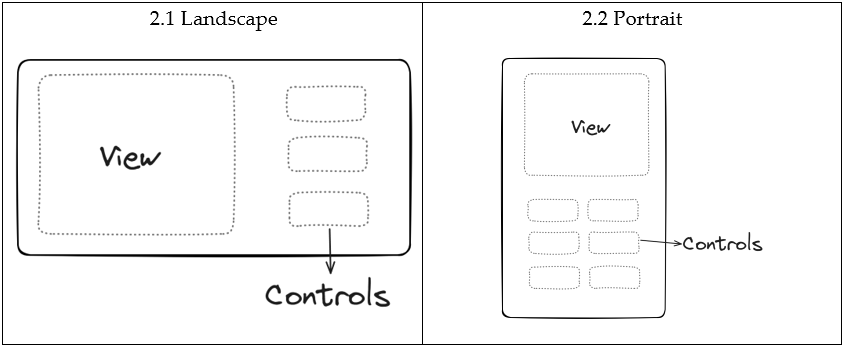
\includegraphics[width=\linewidth]{texs/Part1/chapter3/image/s2.png}
    \caption{Screen Orientation}
    \label{tab:screen-orientation}
\end{table}

\subsection{Battery Type}
\begin{table}[H]
    \centering
    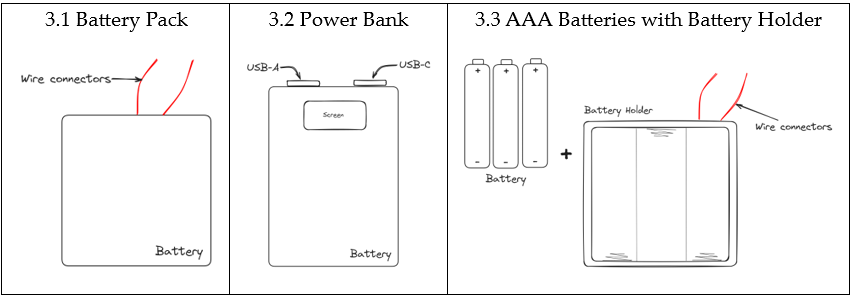
\includegraphics[width=\linewidth]{texs/Part1/chapter3/image/s3.png}
    \caption{Battery Type}
    \label{tab:battery-type}
\end{table}

\subsection{Components Placement}
\begin{table}[H]
    \centering
    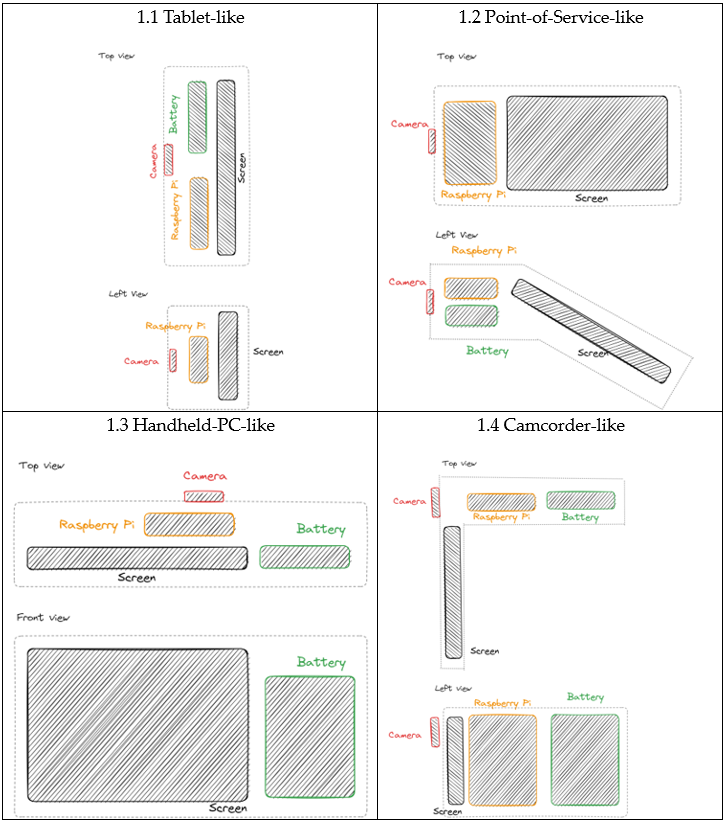
\includegraphics[width=\linewidth]{texs/Part1/chapter3/image/s1.png}
    \caption{Components Placement}
    \label{tab:components-placement}
\end{table}


\subsection{Body Type}
\begin{table}[H]
    \centering
    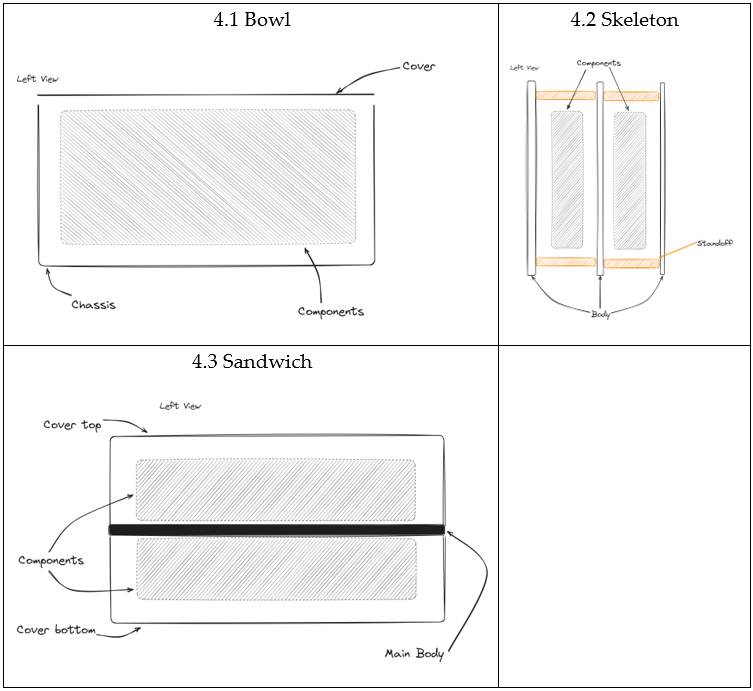
\includegraphics[width=\linewidth]{texs/Part1/chapter3/image/s4.png}
    \caption{Body Type}
    \label{tab:body-type}
\end{table}

\subsection{Handling}
\begin{table}[H]
    \centering
    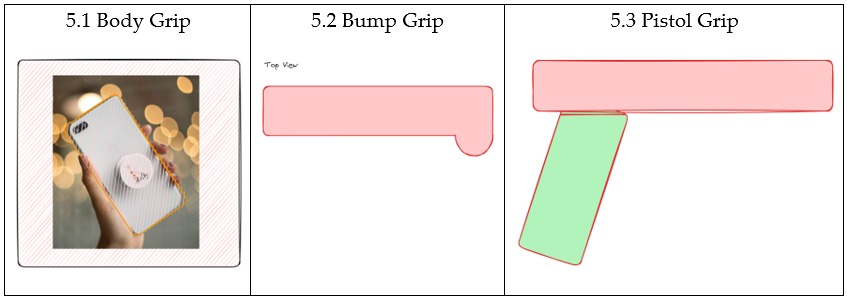
\includegraphics[width=\linewidth]{texs/Part1/chapter3/image/s5.png}
    \caption{Handling}
    \label{tab:handling}
\end{table}

\subsection{External Mounting}
\begin{table}[H]
    \centering
    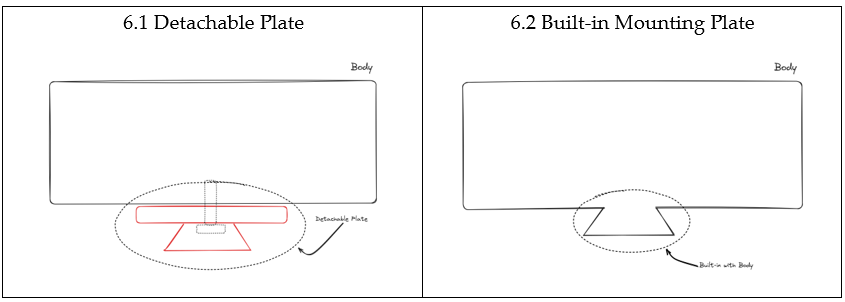
\includegraphics[width=\linewidth]{texs/Part1/chapter3/image/s6.png}
    \caption{External Mounting}
    \label{tab:external-mounting}
\end{table}

\subsection{Control Mechanism}
\begin{table}[H]
    \centering
    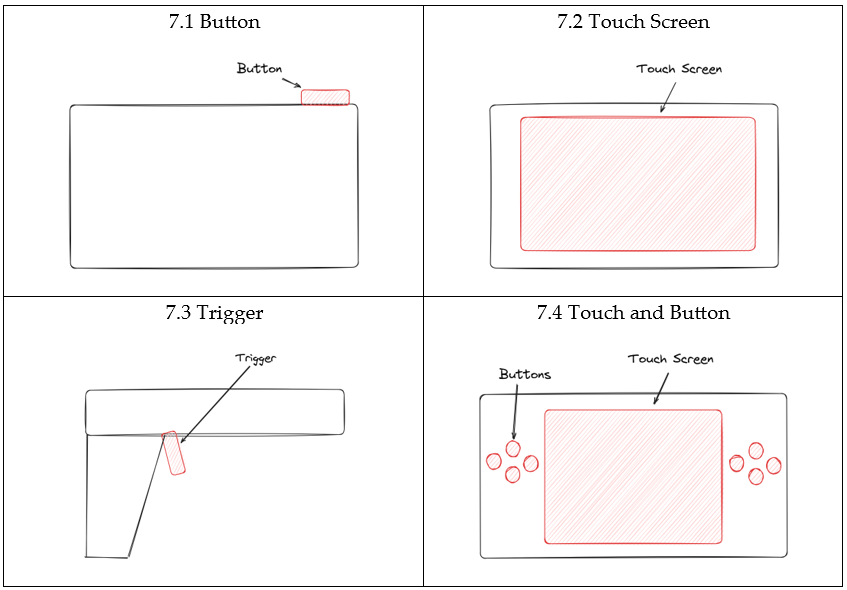
\includegraphics[width=\linewidth]{texs/Part1/chapter3/image/s7.png}
    \caption{Control Mechanism}
    \label{tab:control-mechanism}
\end{table}

\section{CAD Drawings}
\label{appendix:cad-drawings}

\begin{figure}[H]
    \centering
    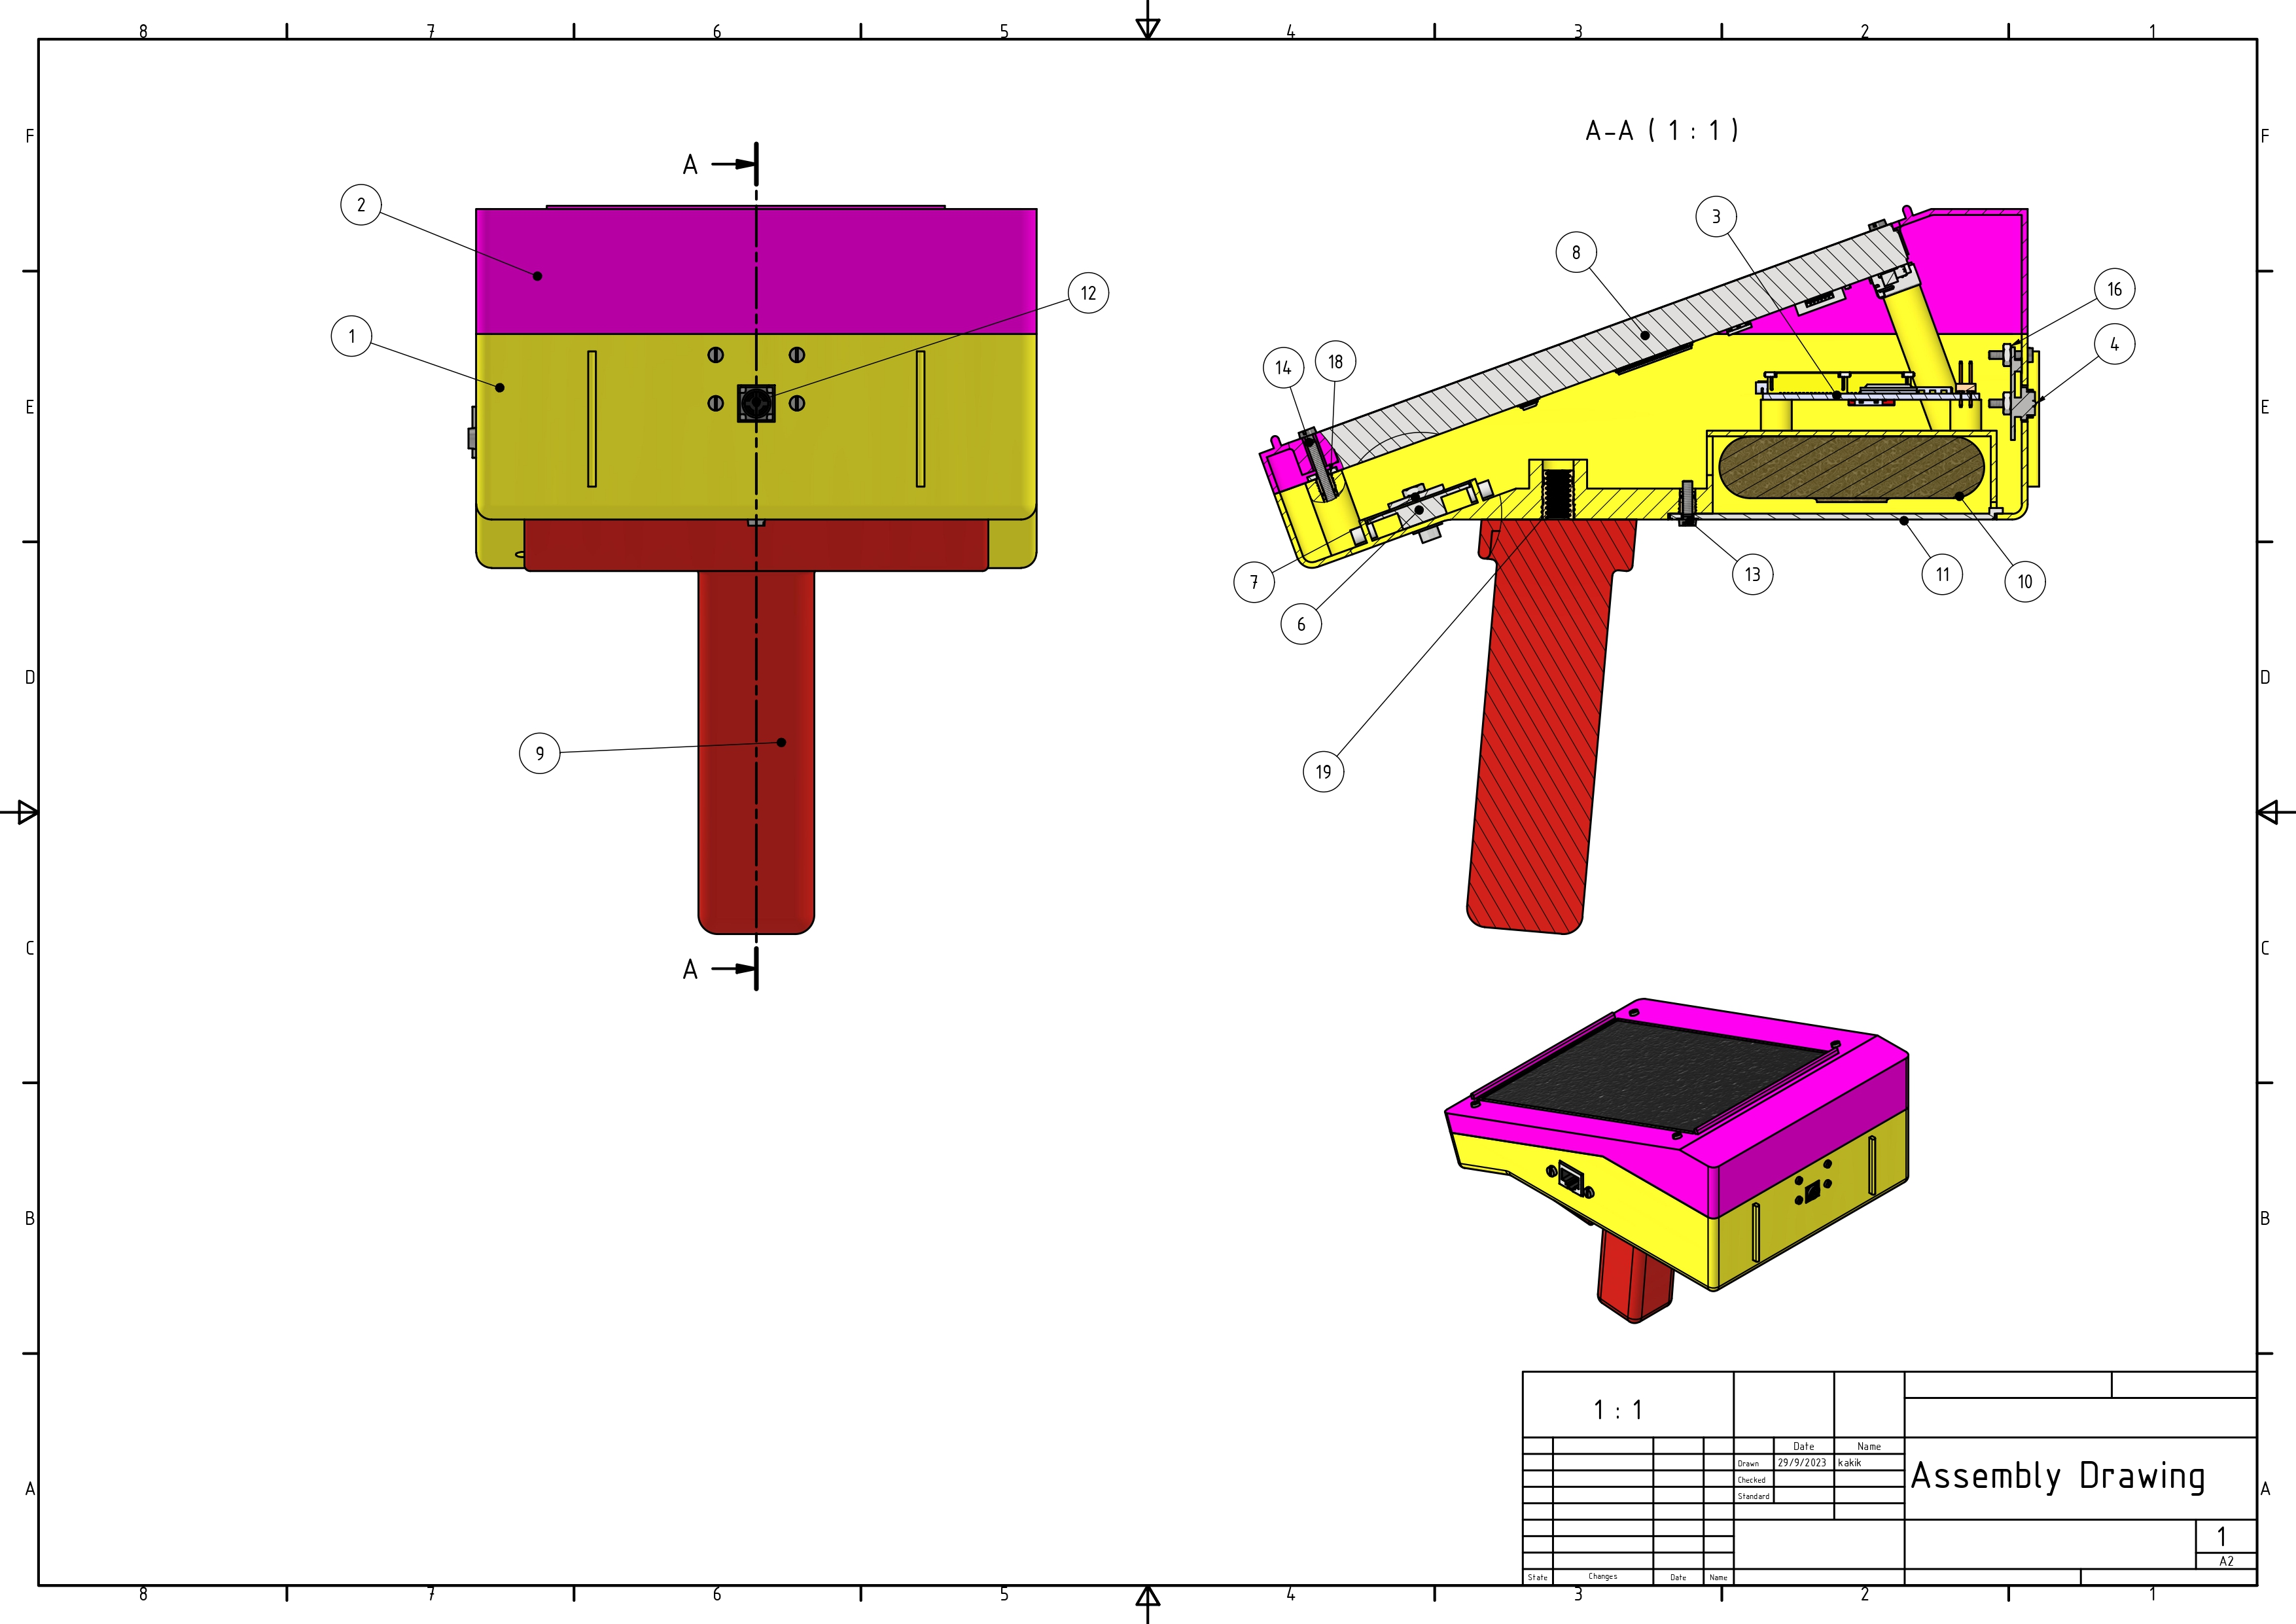
\includegraphics[width=1.2\linewidth, angle = 90]{texs/appendix/data/technicaldrawing/assembly.jpg}
    \caption{Assembly Drawing}
    \label{fig:cad-drawing-assembly}
\end{figure}

\begin{figure}[H]
    \centering
    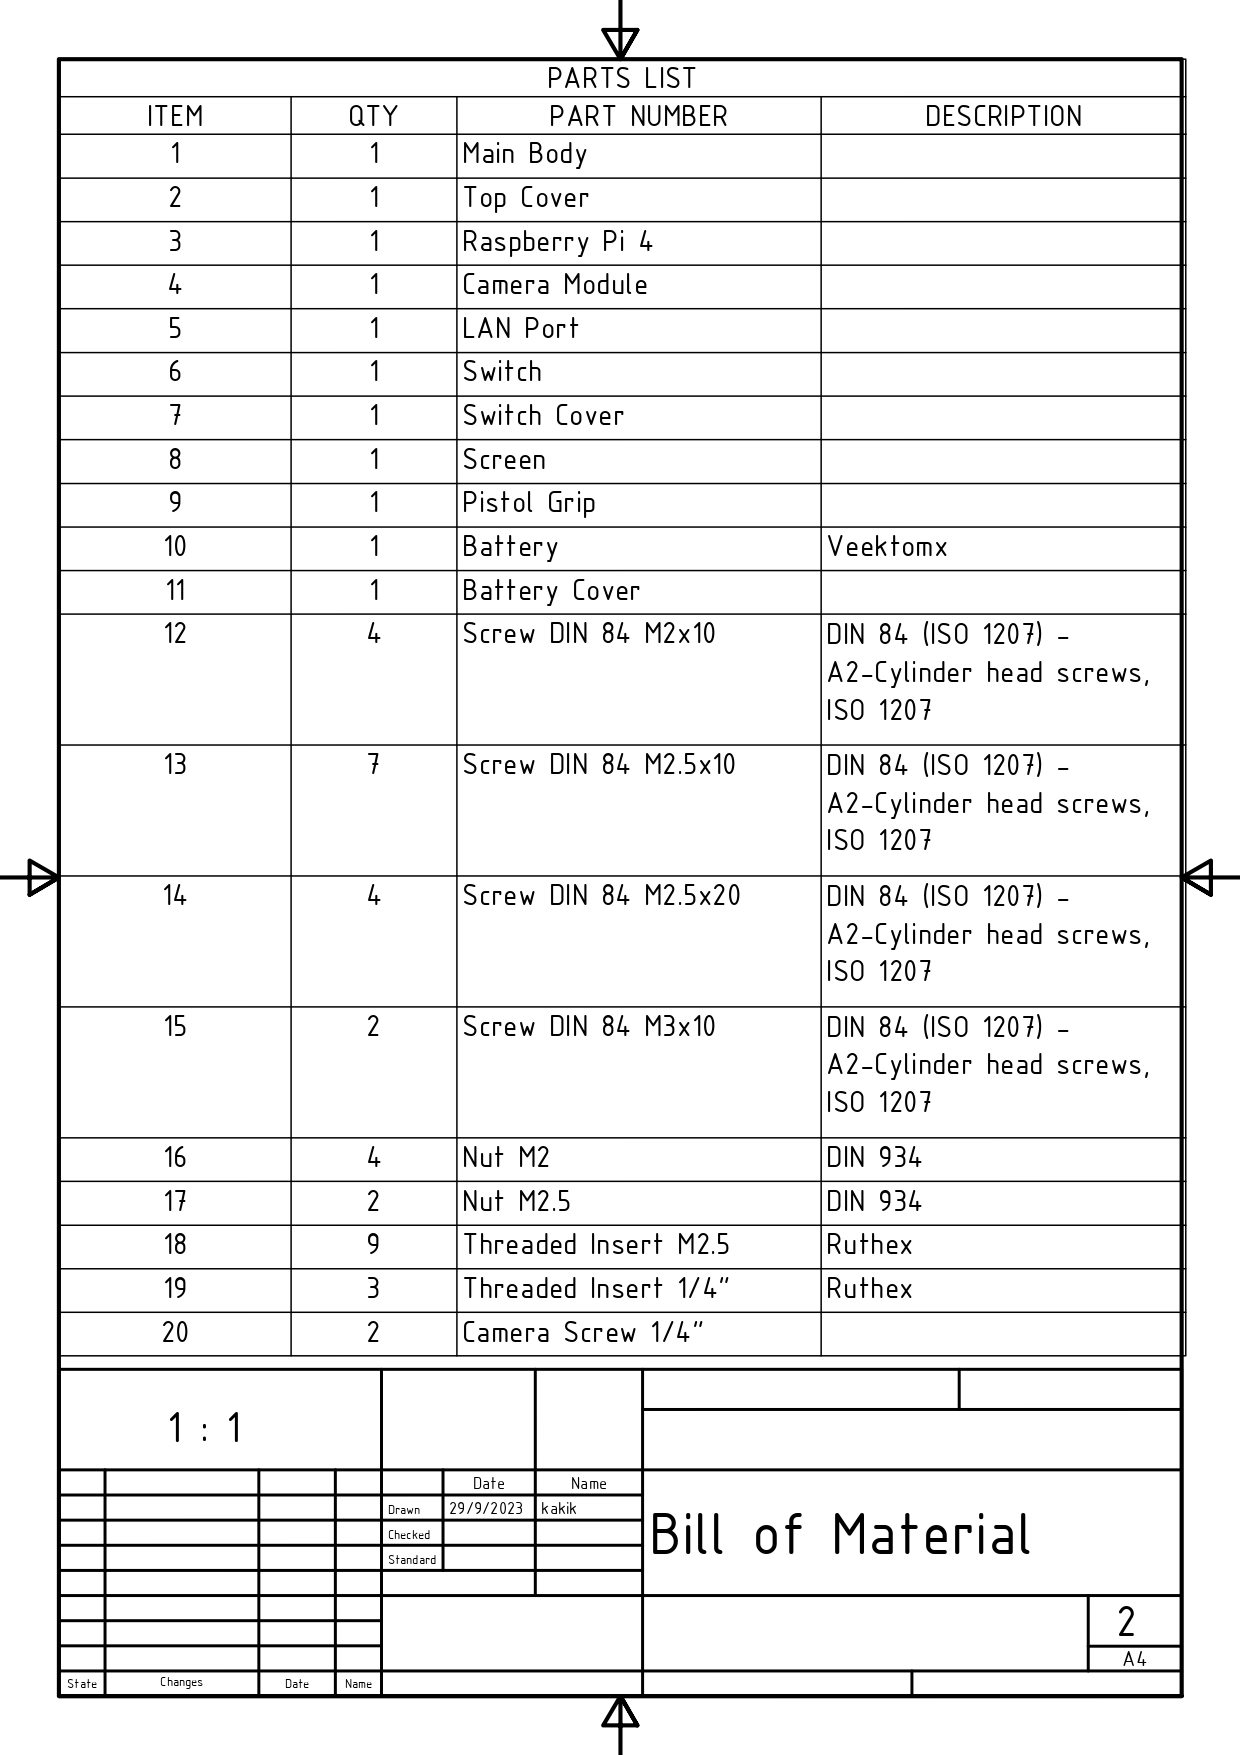
\includegraphics[width=0.9\linewidth]{texs/appendix/data/technicaldrawing/bom.jpg}
    \caption{Bill of Materials}
    \label{fig:cad-drawing-bom}
\end{figure}

\begin{figure}[H]
    \centering
    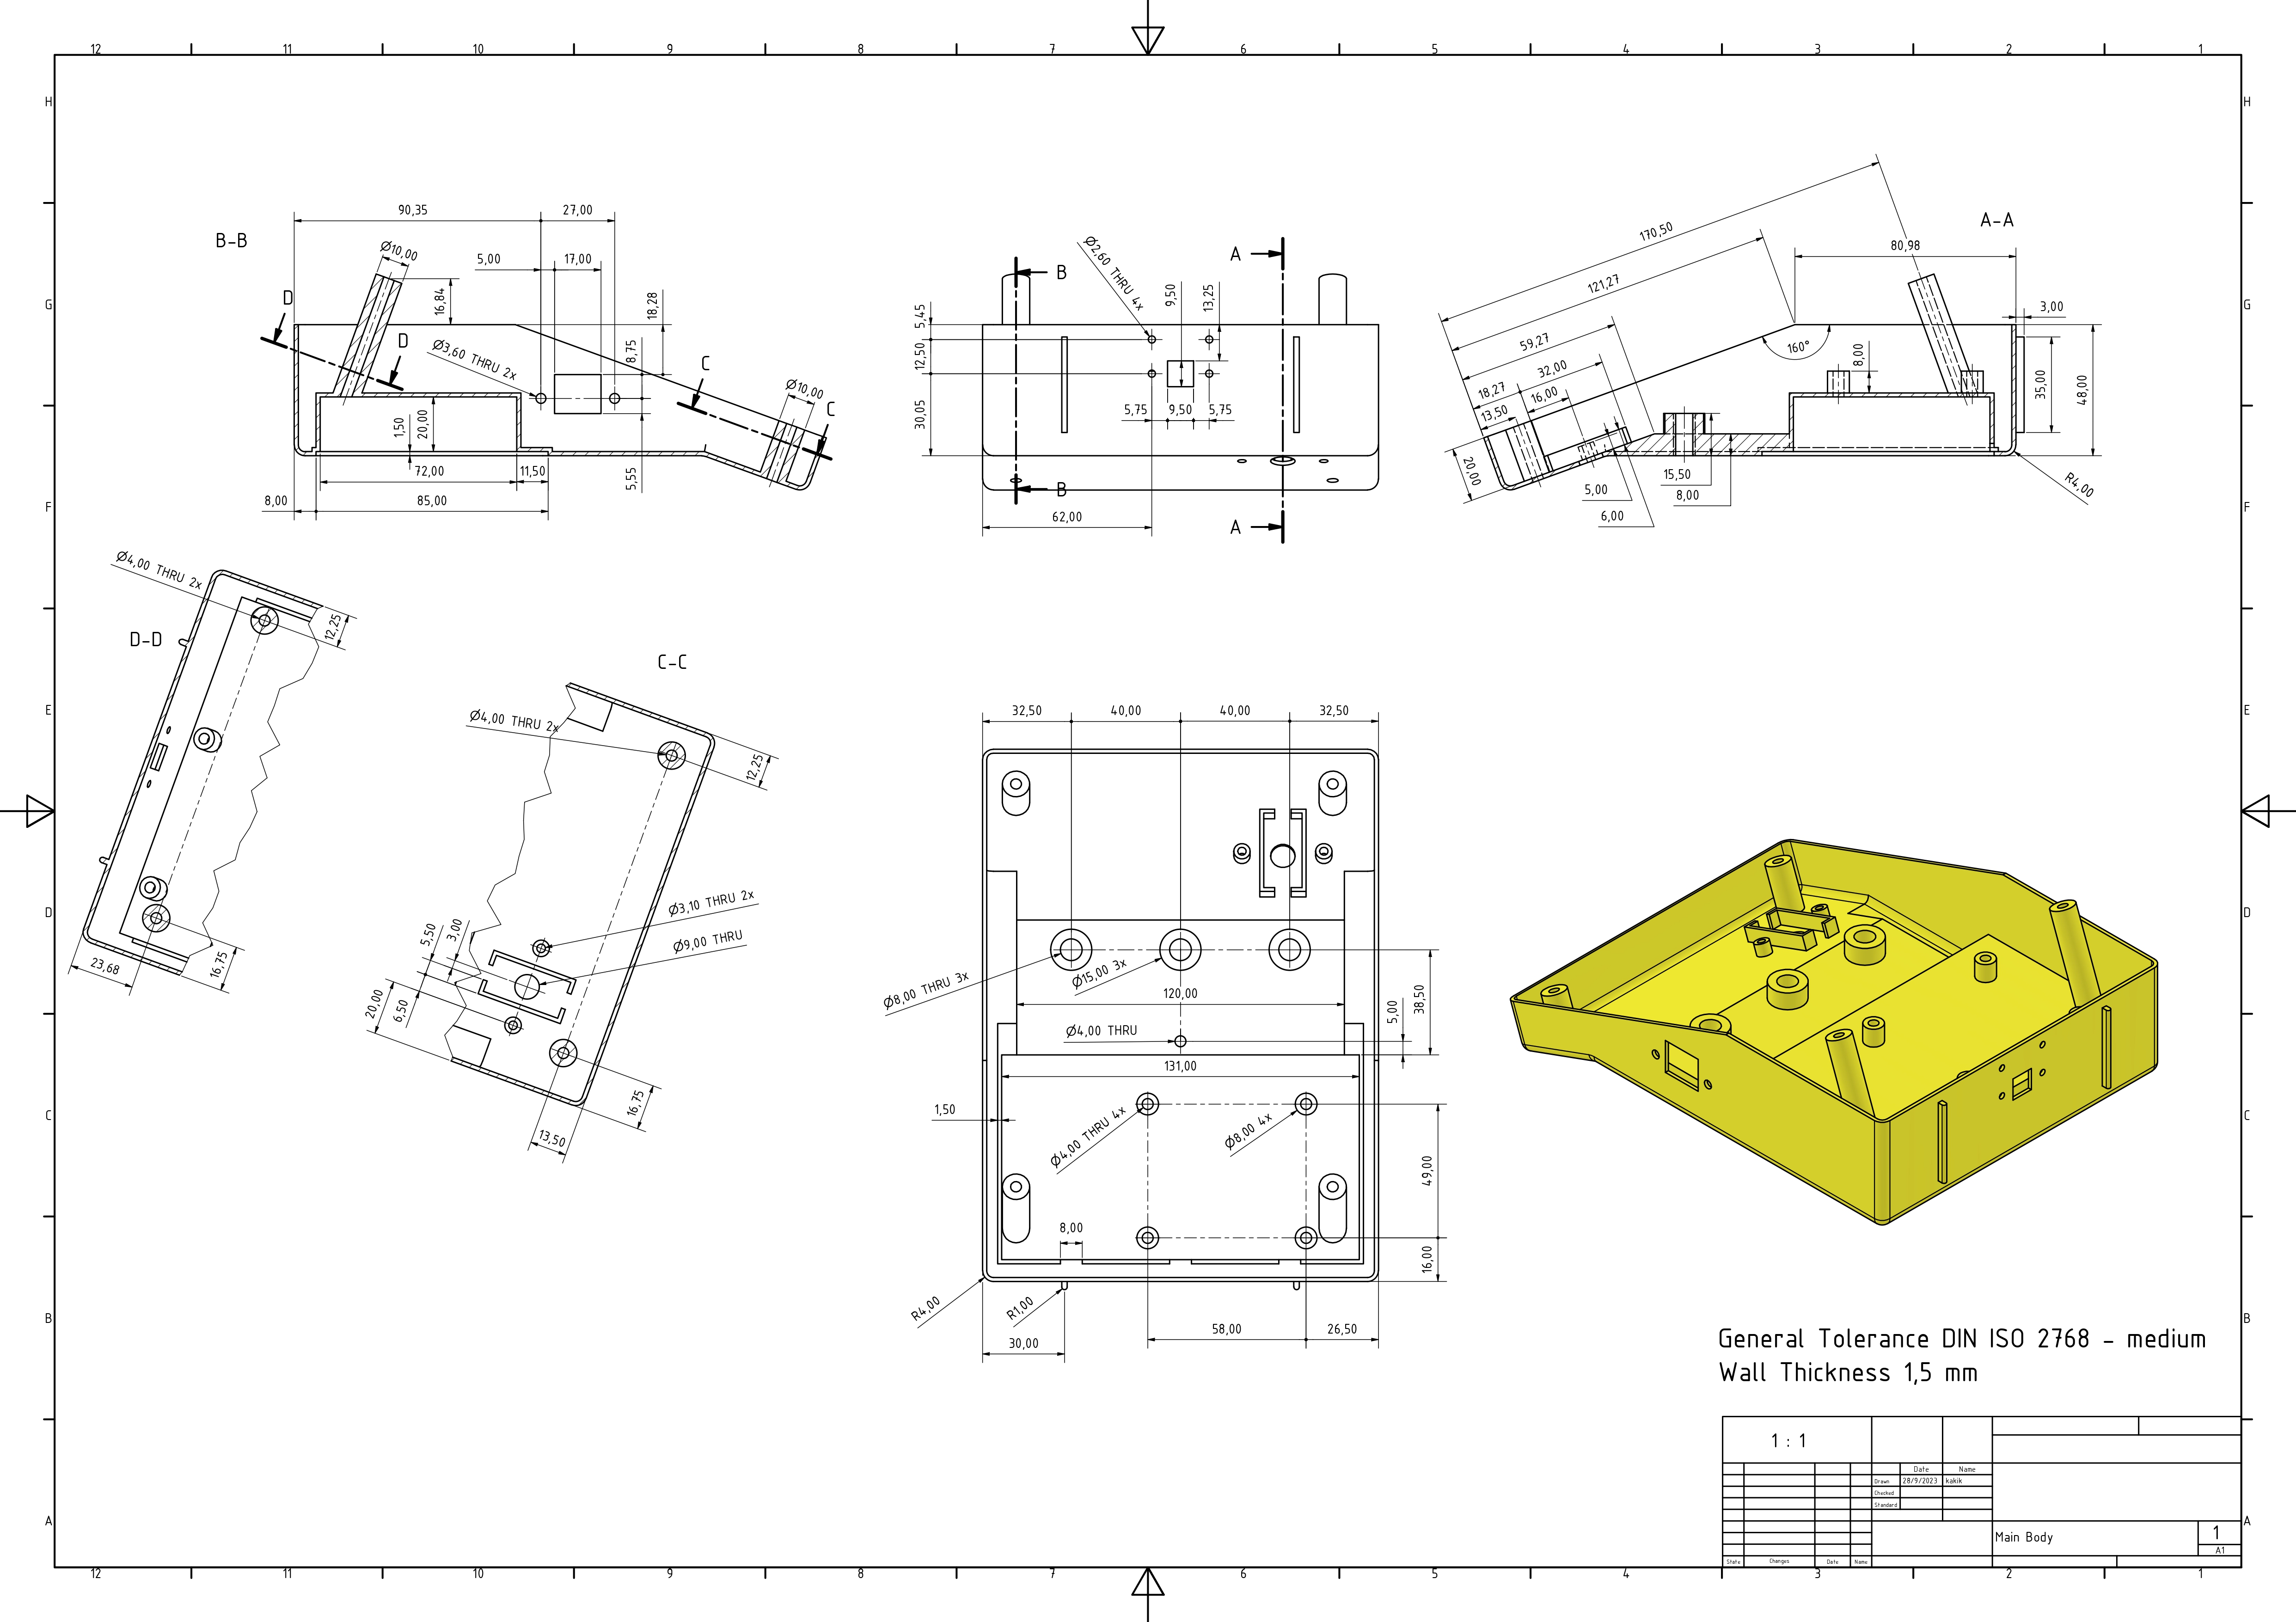
\includegraphics[width=1.3\linewidth, angle = 90]{texs/appendix/data/technicaldrawing/mainbody.jpg}
    \caption{Main Body Drawing}
    \label{fig:cad-drawing-mainbody}
\end{figure}

\begin{figure}[H]
    \centering
    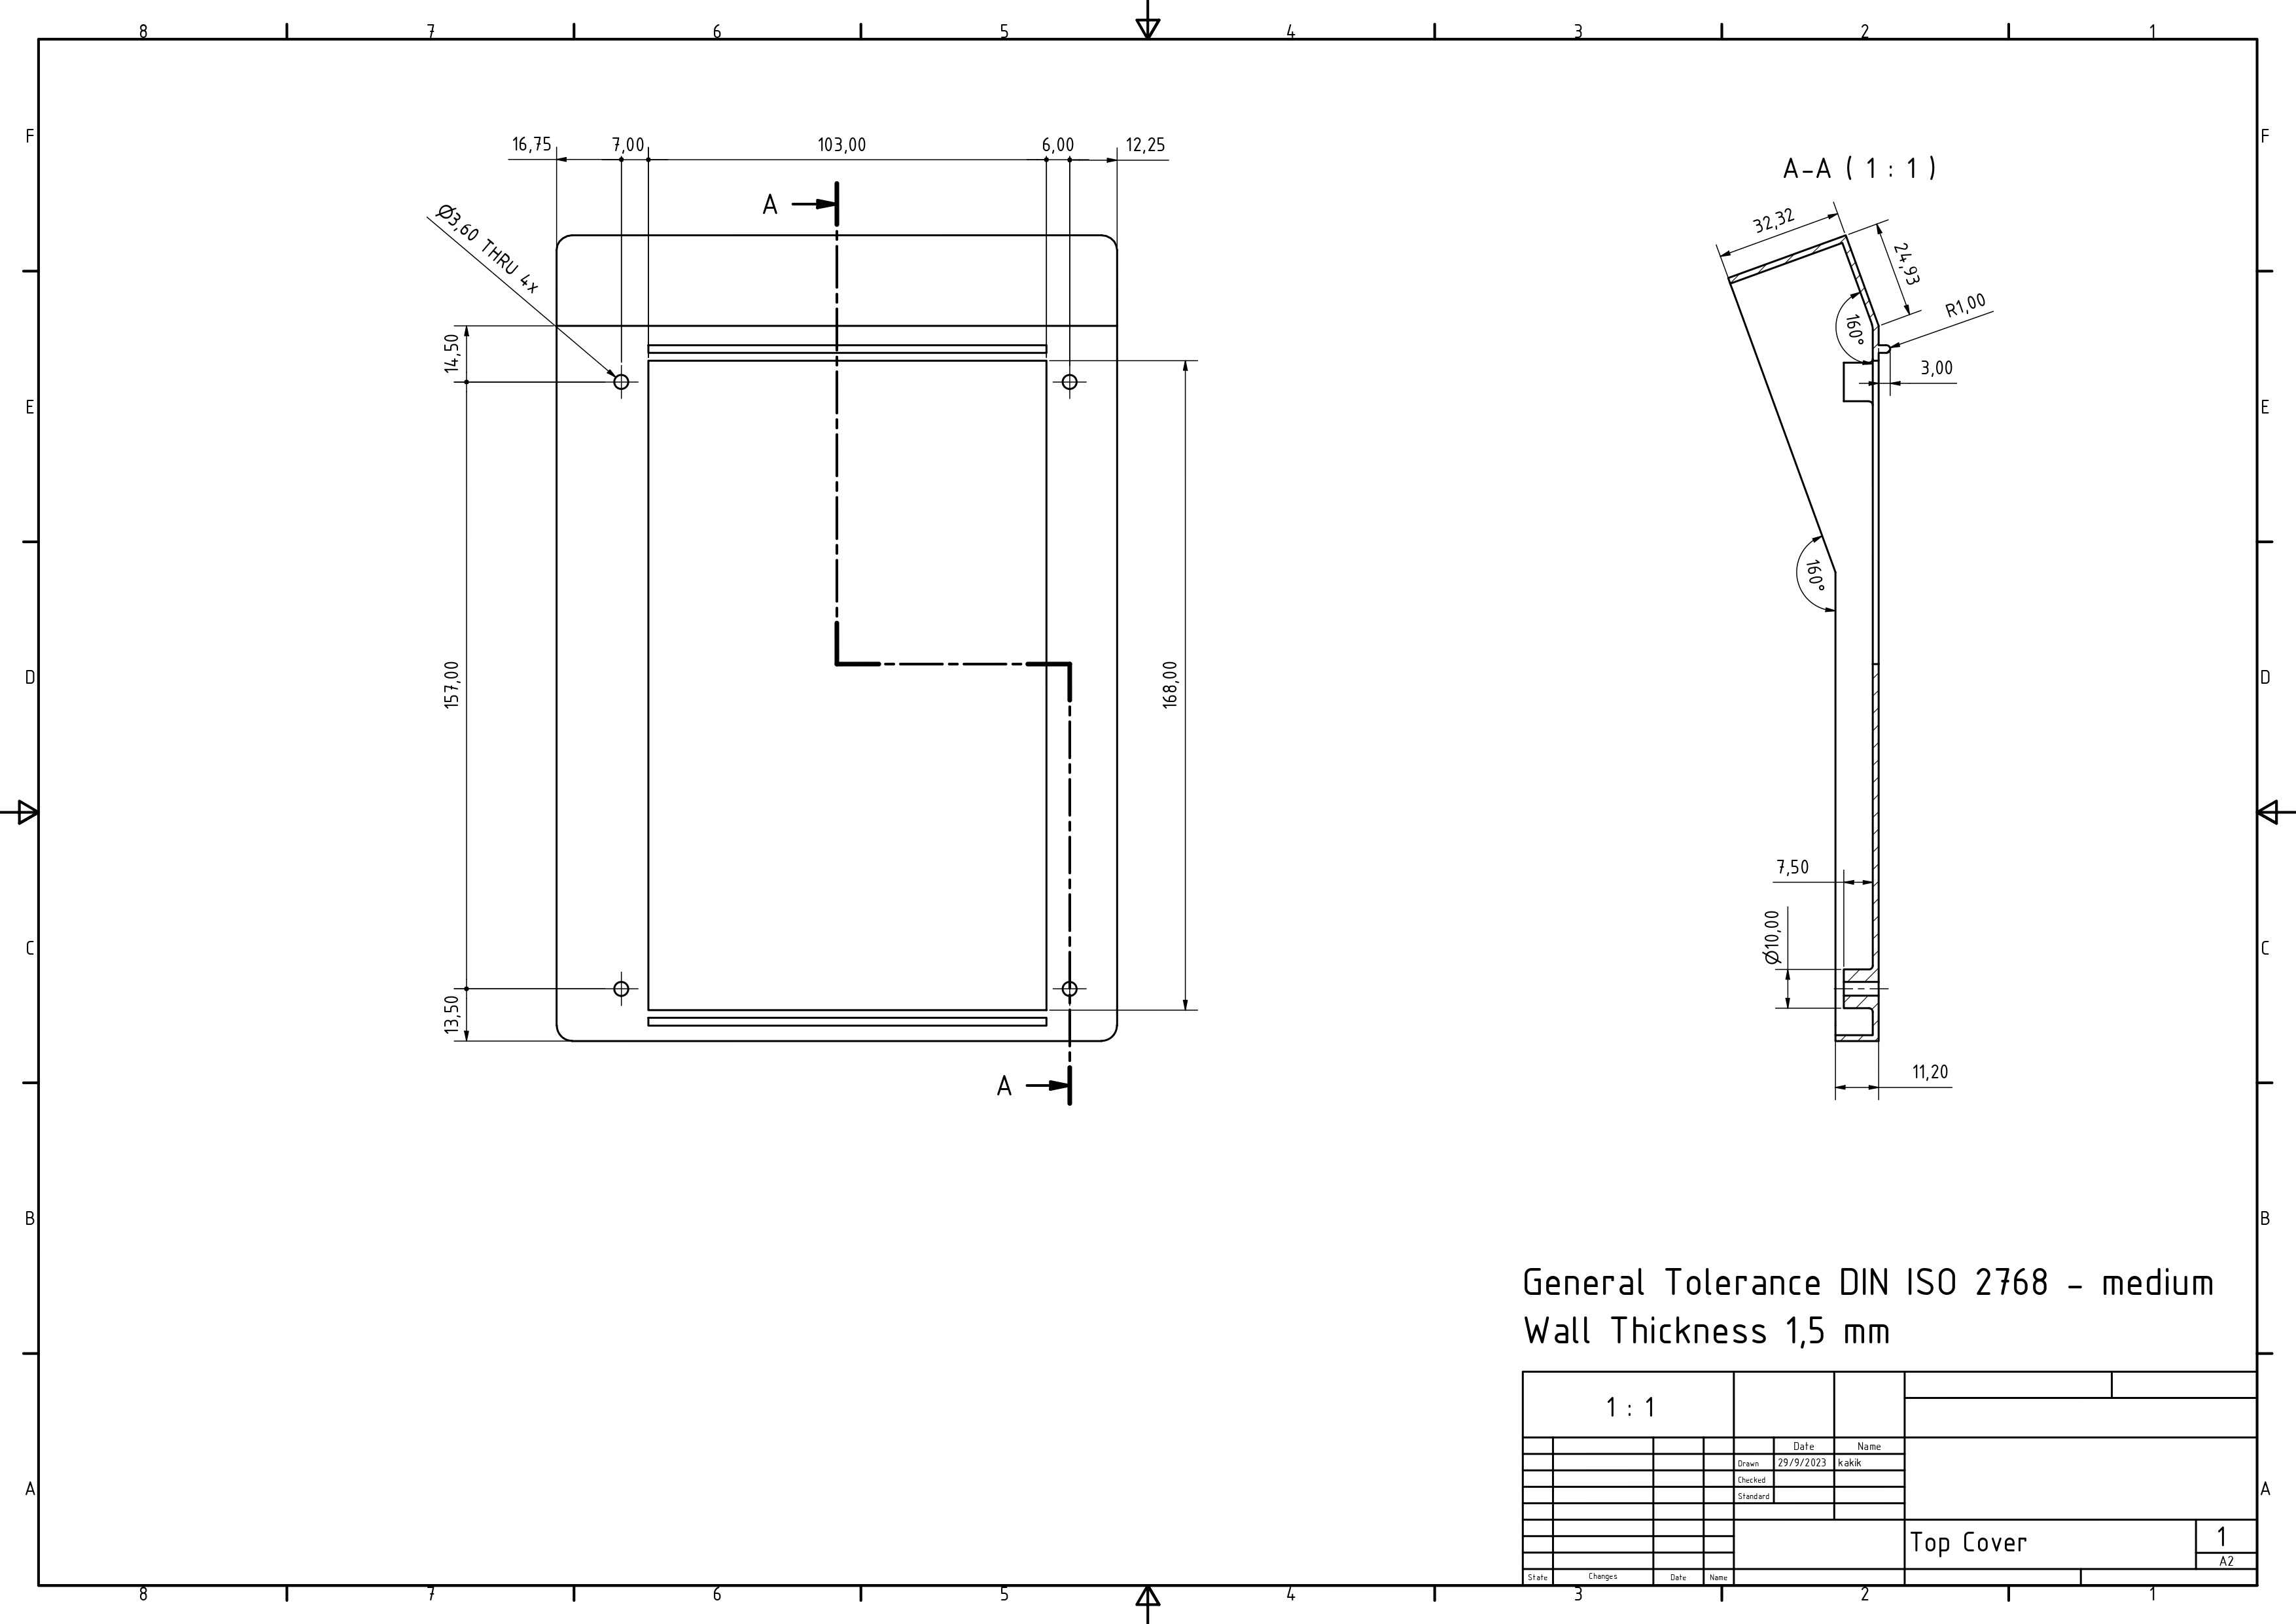
\includegraphics[width=1.3\linewidth, angle = 90]{texs/appendix/data/technicaldrawing/topcover.jpg}
    \caption{Top Cover Drawing}
    \label{fig:cad-drawing-topcover}
\end{figure}

\begin{figure}[H]
    \centering
    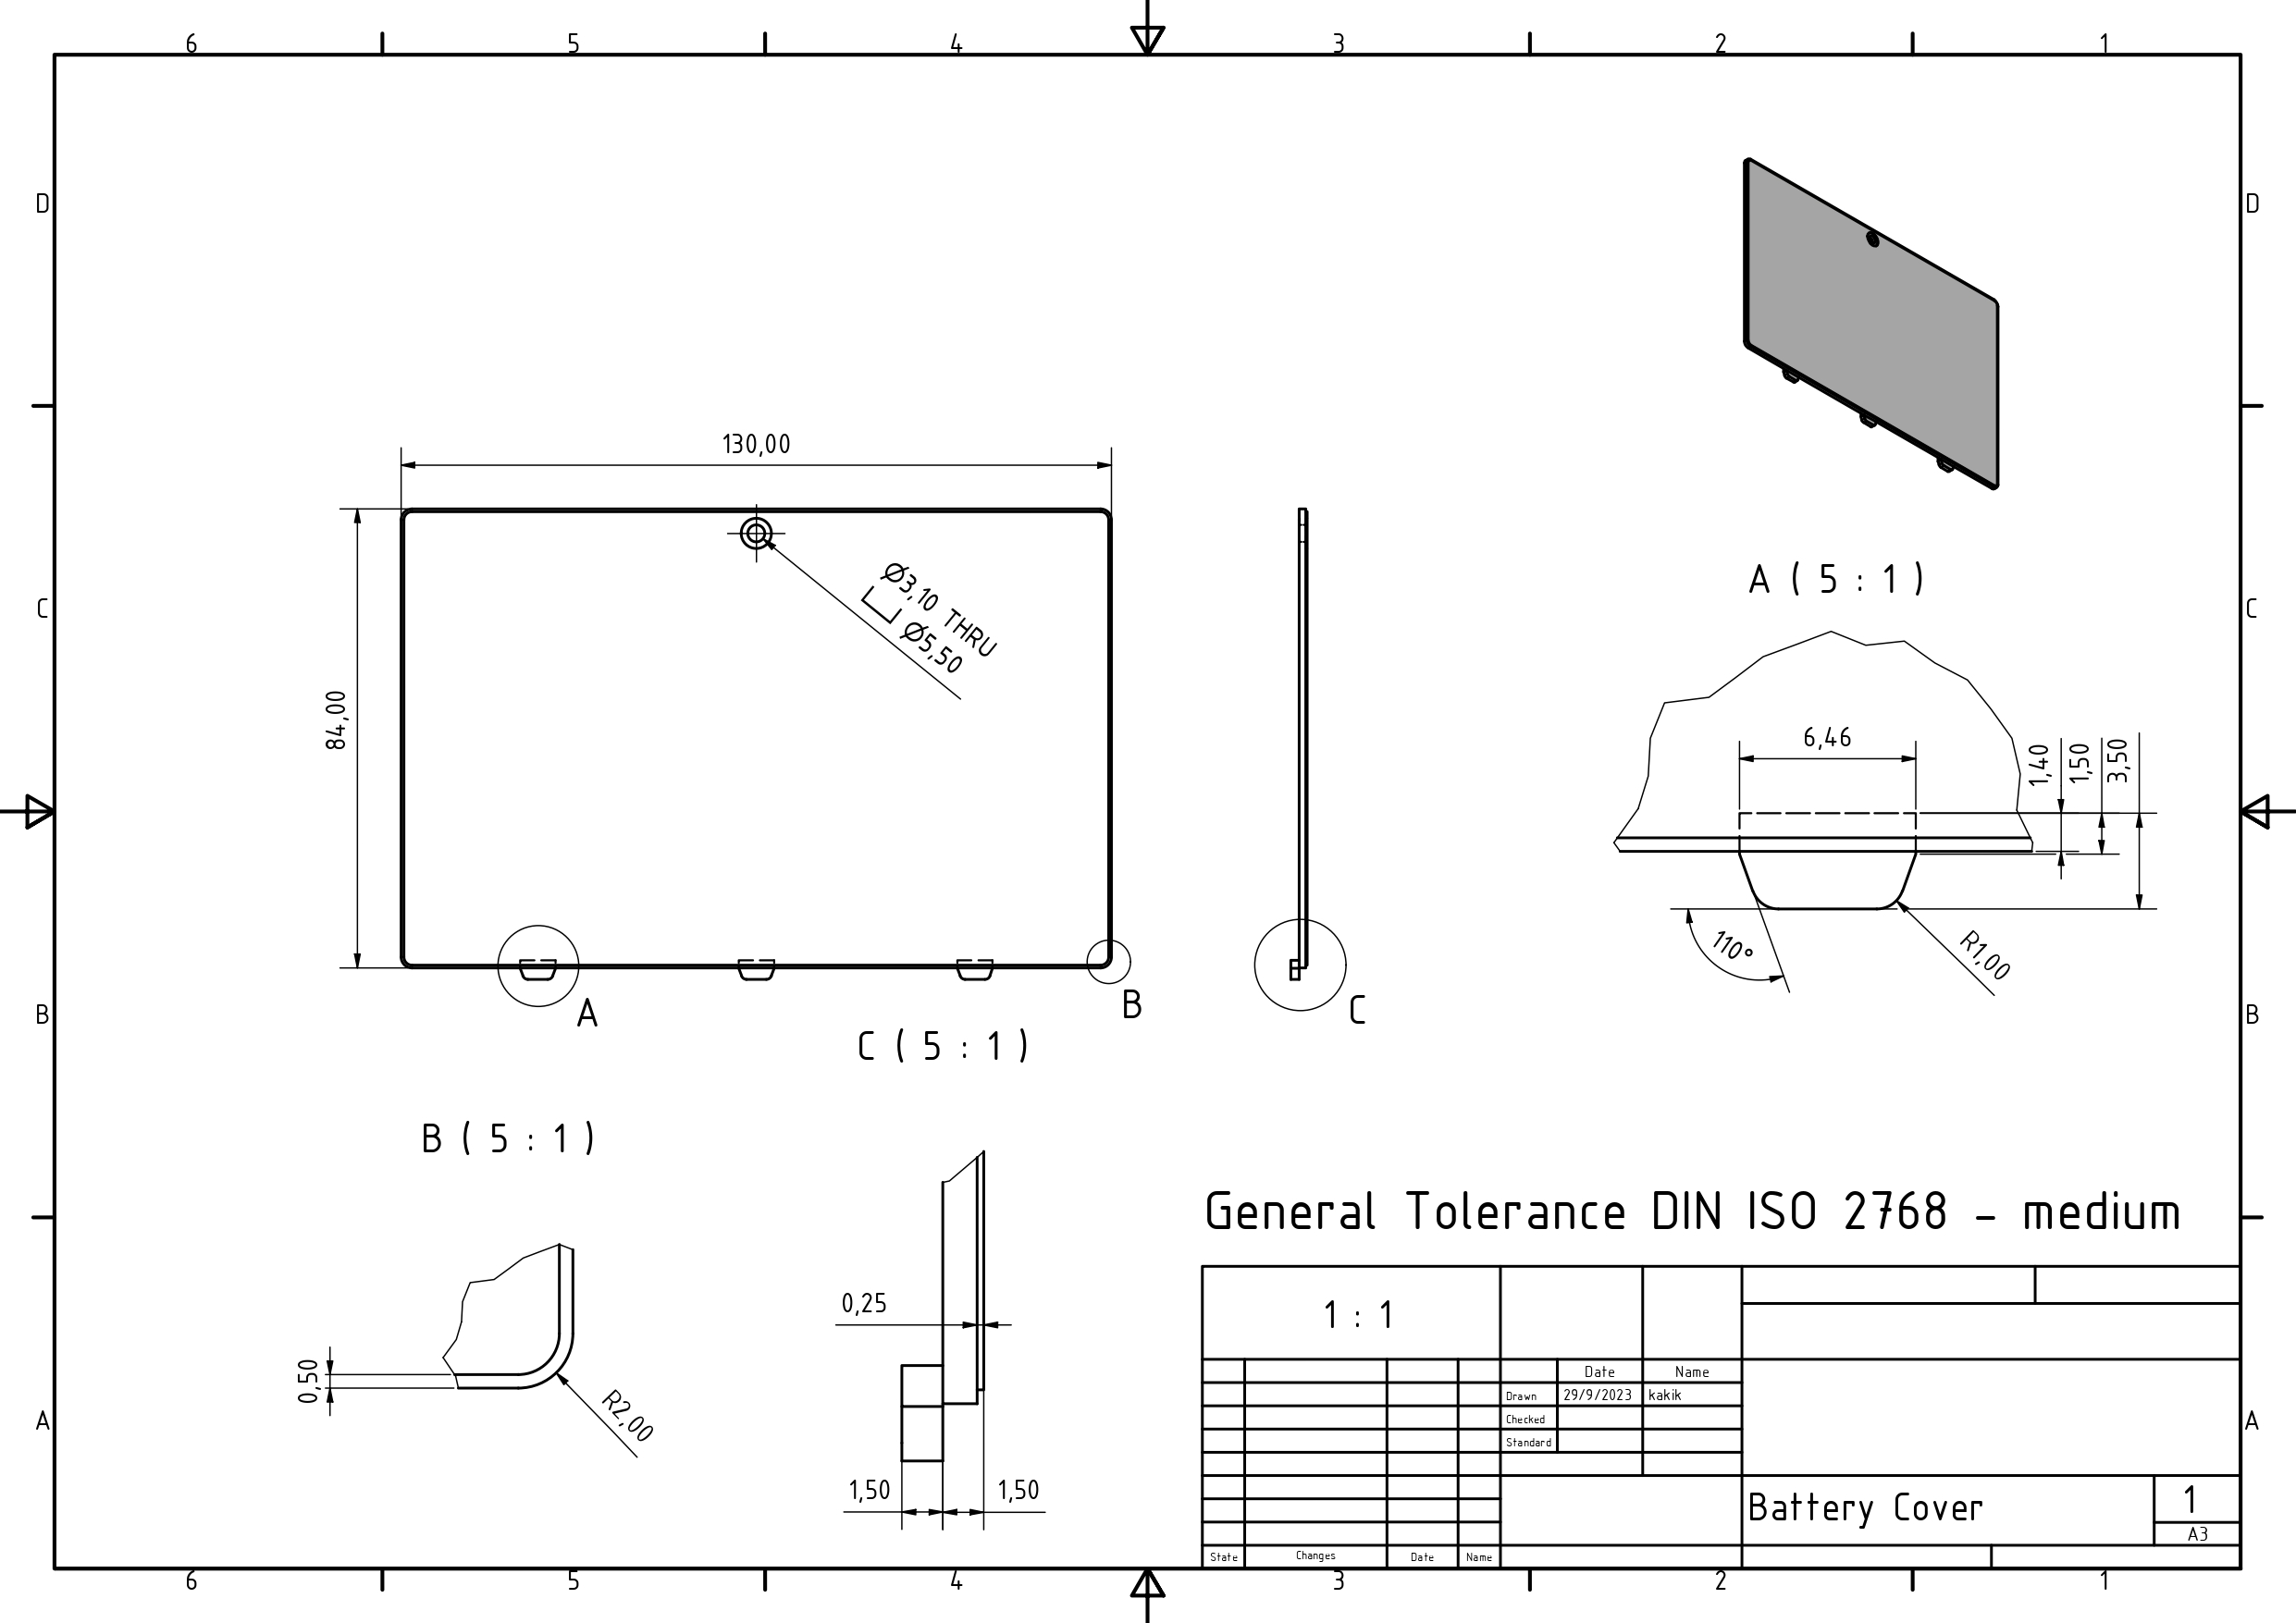
\includegraphics[width=1.3\linewidth, angle = 90]{texs/appendix/data/technicaldrawing/batterycover.jpg}
    \caption{Battery Cover Drawing}
    \label{fig:cad-drawing-batterycover}
\end{figure}

\begin{figure}[H]
    \centering
    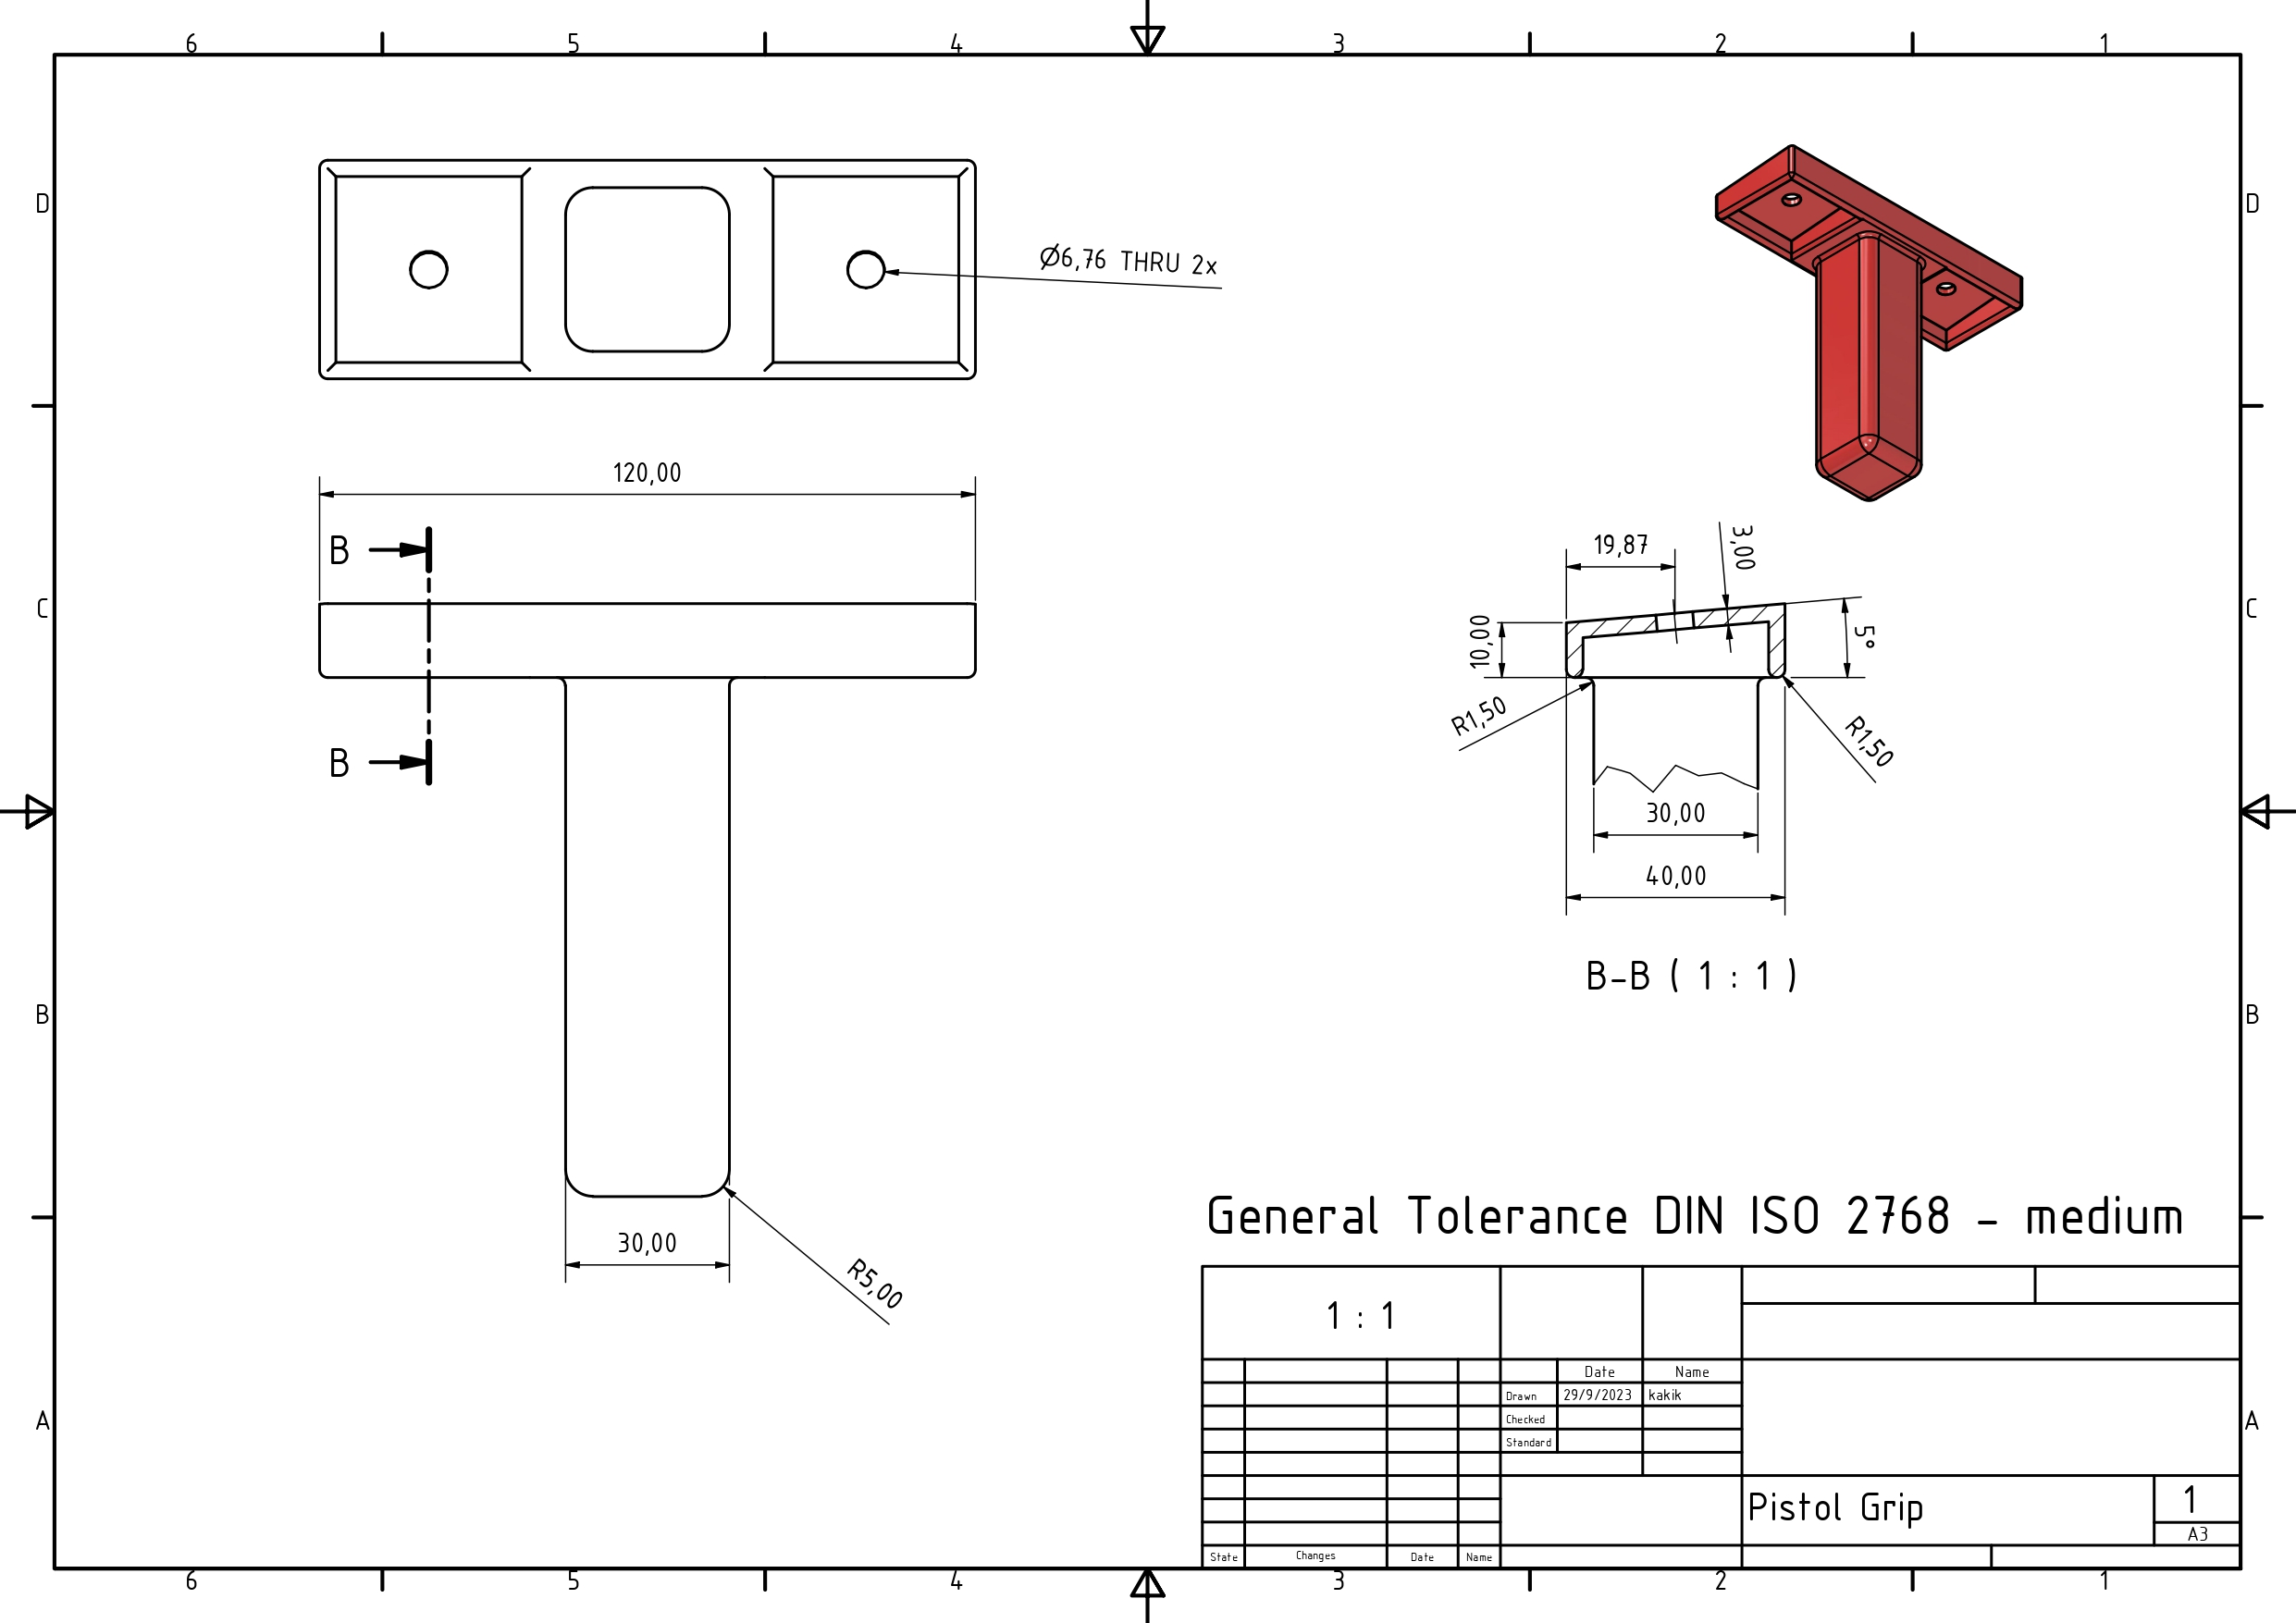
\includegraphics[width=1.3\linewidth, angle = 90]{texs/appendix/data/technicaldrawing/pistolgrip.jpg}
    \caption{Pistol Grip Drawing}
    \label{fig:cad-drawing-pistolgrip}
\end{figure}

\begin{figure}[H]
    \centering
    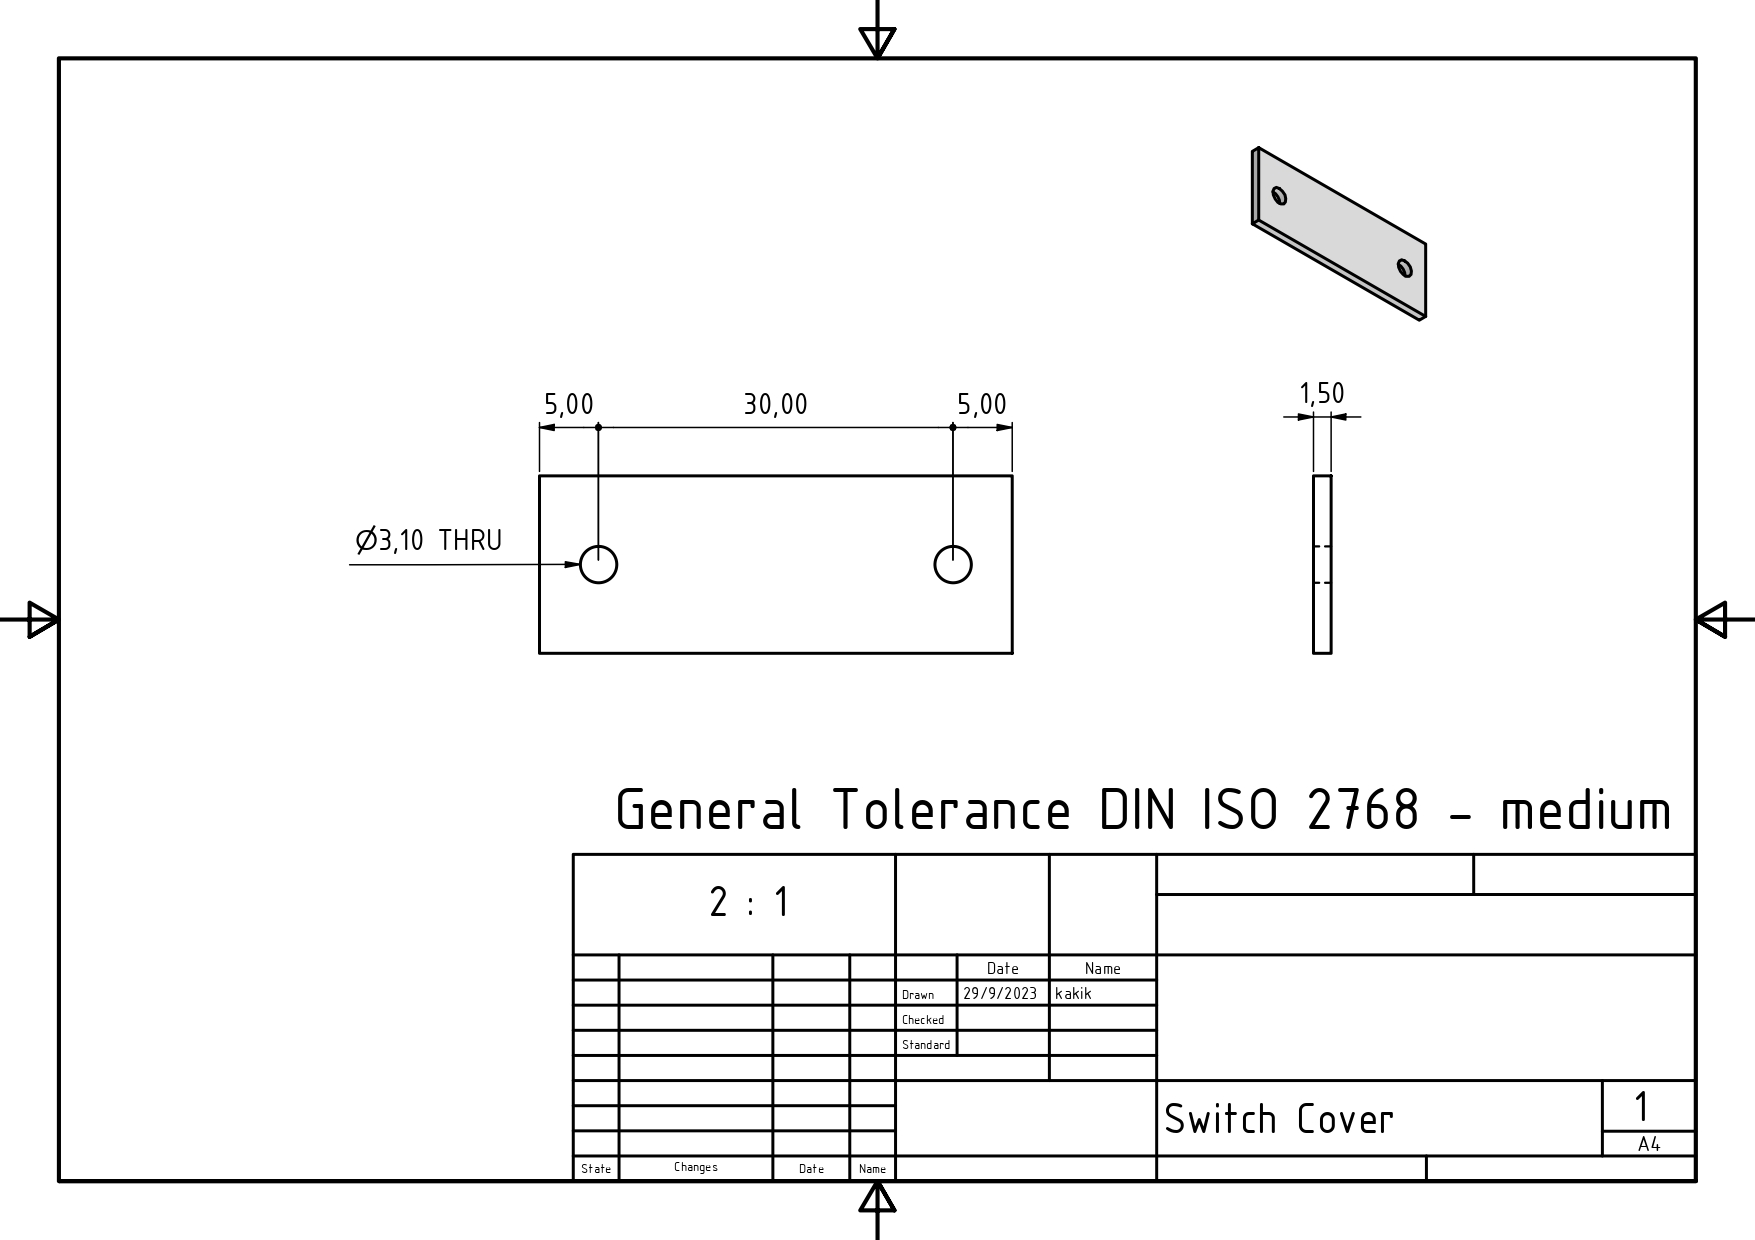
\includegraphics[width=1.3\linewidth, angle = 90]{texs/appendix/data/technicaldrawing/switchcover.jpg}
    \caption{Switch Cover Drawing}
    \label{fig:cad-drawing-switchcover}
\end{figure}

\section{Technical Specifications}
\subsection{Original Prusa i3 MK3S+ 3D printer}
\label{appendix:original-prusa-i3-mk3s-3d-printer}

\begin{figure}[H]
    \centering
    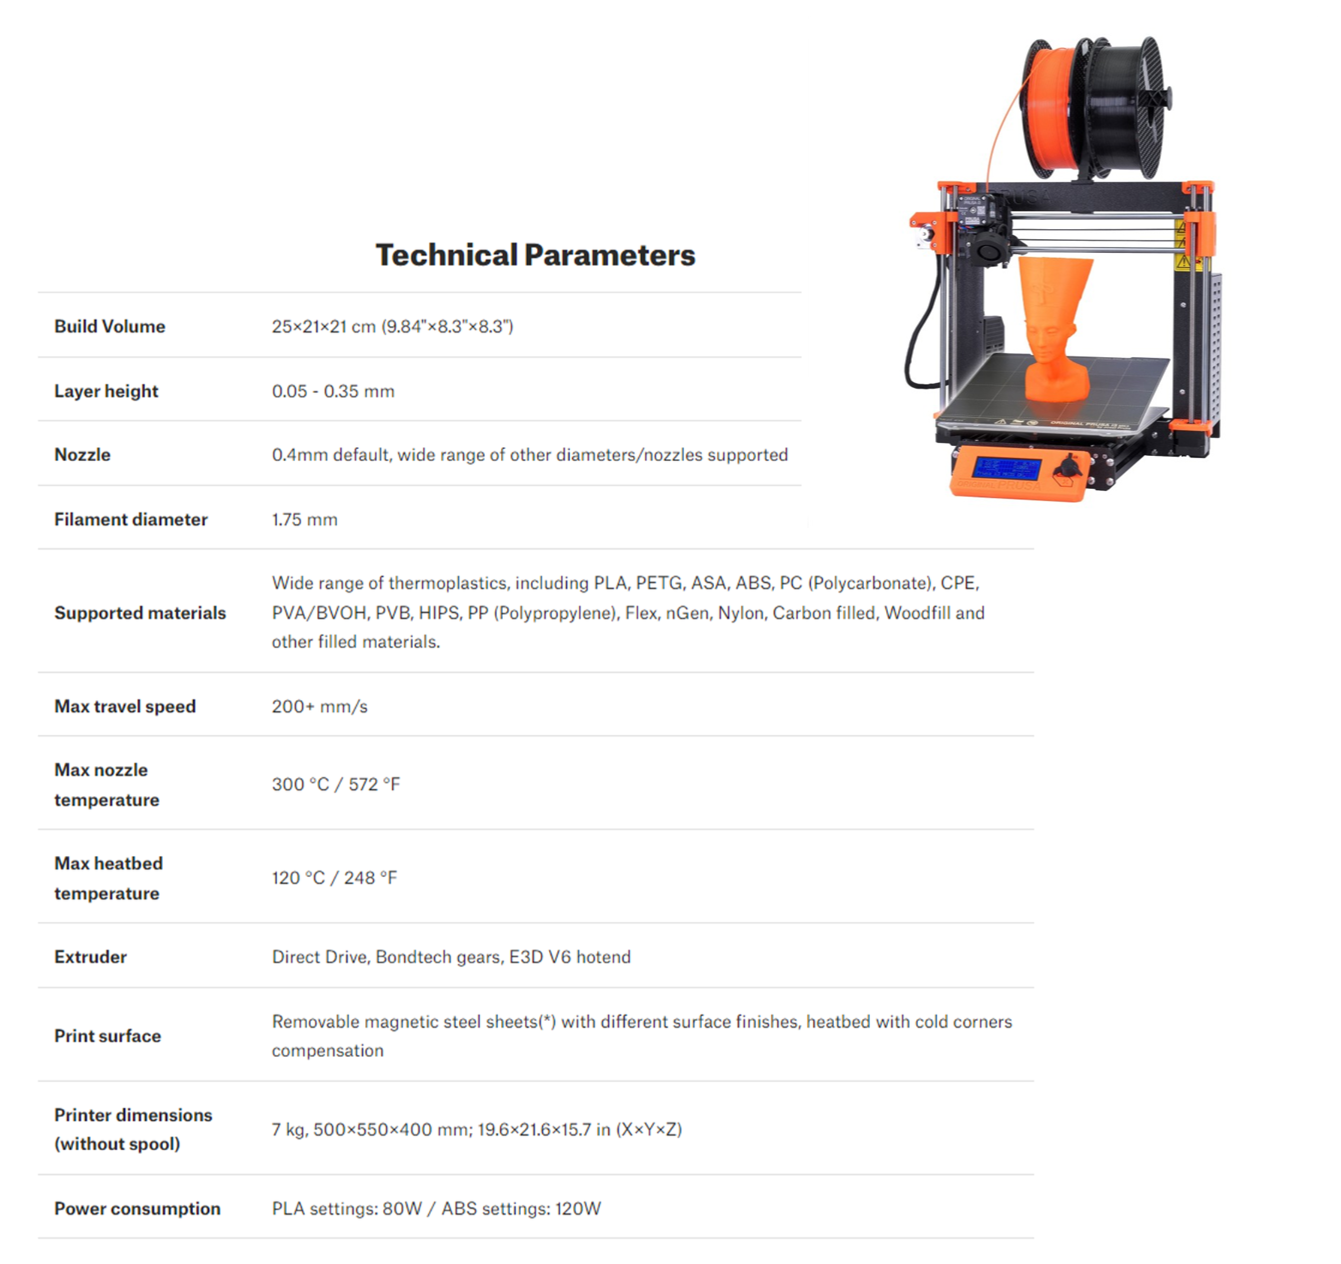
\includegraphics[width=\linewidth]{texs/appendix/data/techspecs/prusa.png}
    \caption{Original Prusa i3 MK3S+ 3D printer}
    \label{fig:3d-printer-1}
\end{figure}

\subsection{Raspberry Pi 4 Model B}
\label{appendix:raspberry-pi-4-model-b}

\begin{figure}[H]
    \centering
    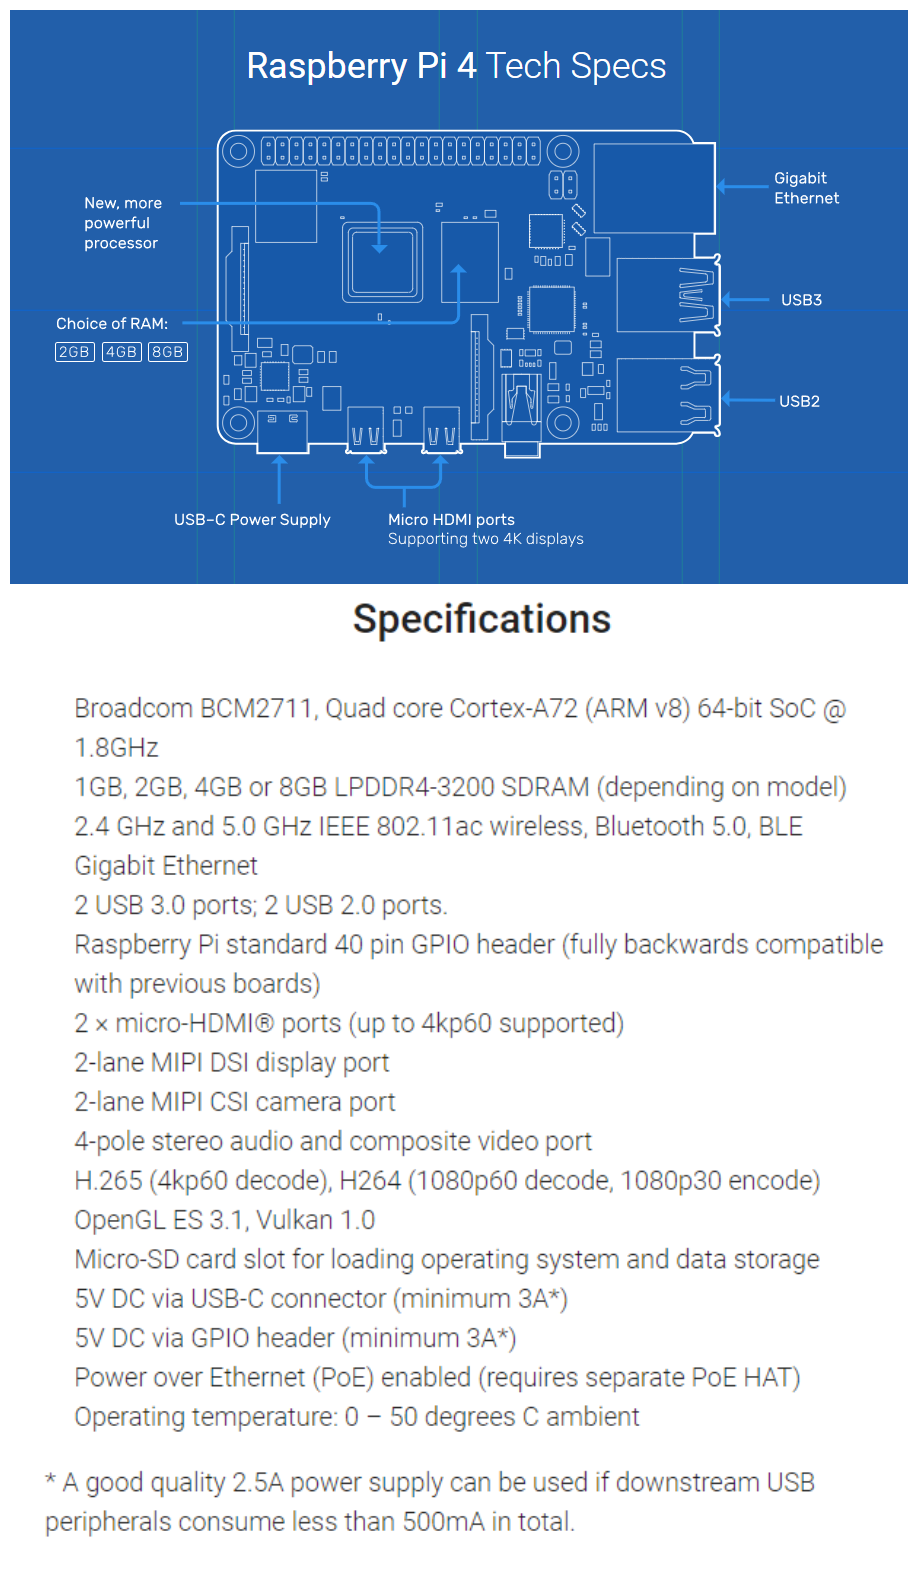
\includegraphics[width=0.7\linewidth]{texs/appendix/data/techspecs/pi-specs.png}
    \caption{Raspberry Pi 4 Model B Technical Specifications}
    \label{fig:rpi-1}
\end{figure}

\begin{figure}[H]
    \centering
    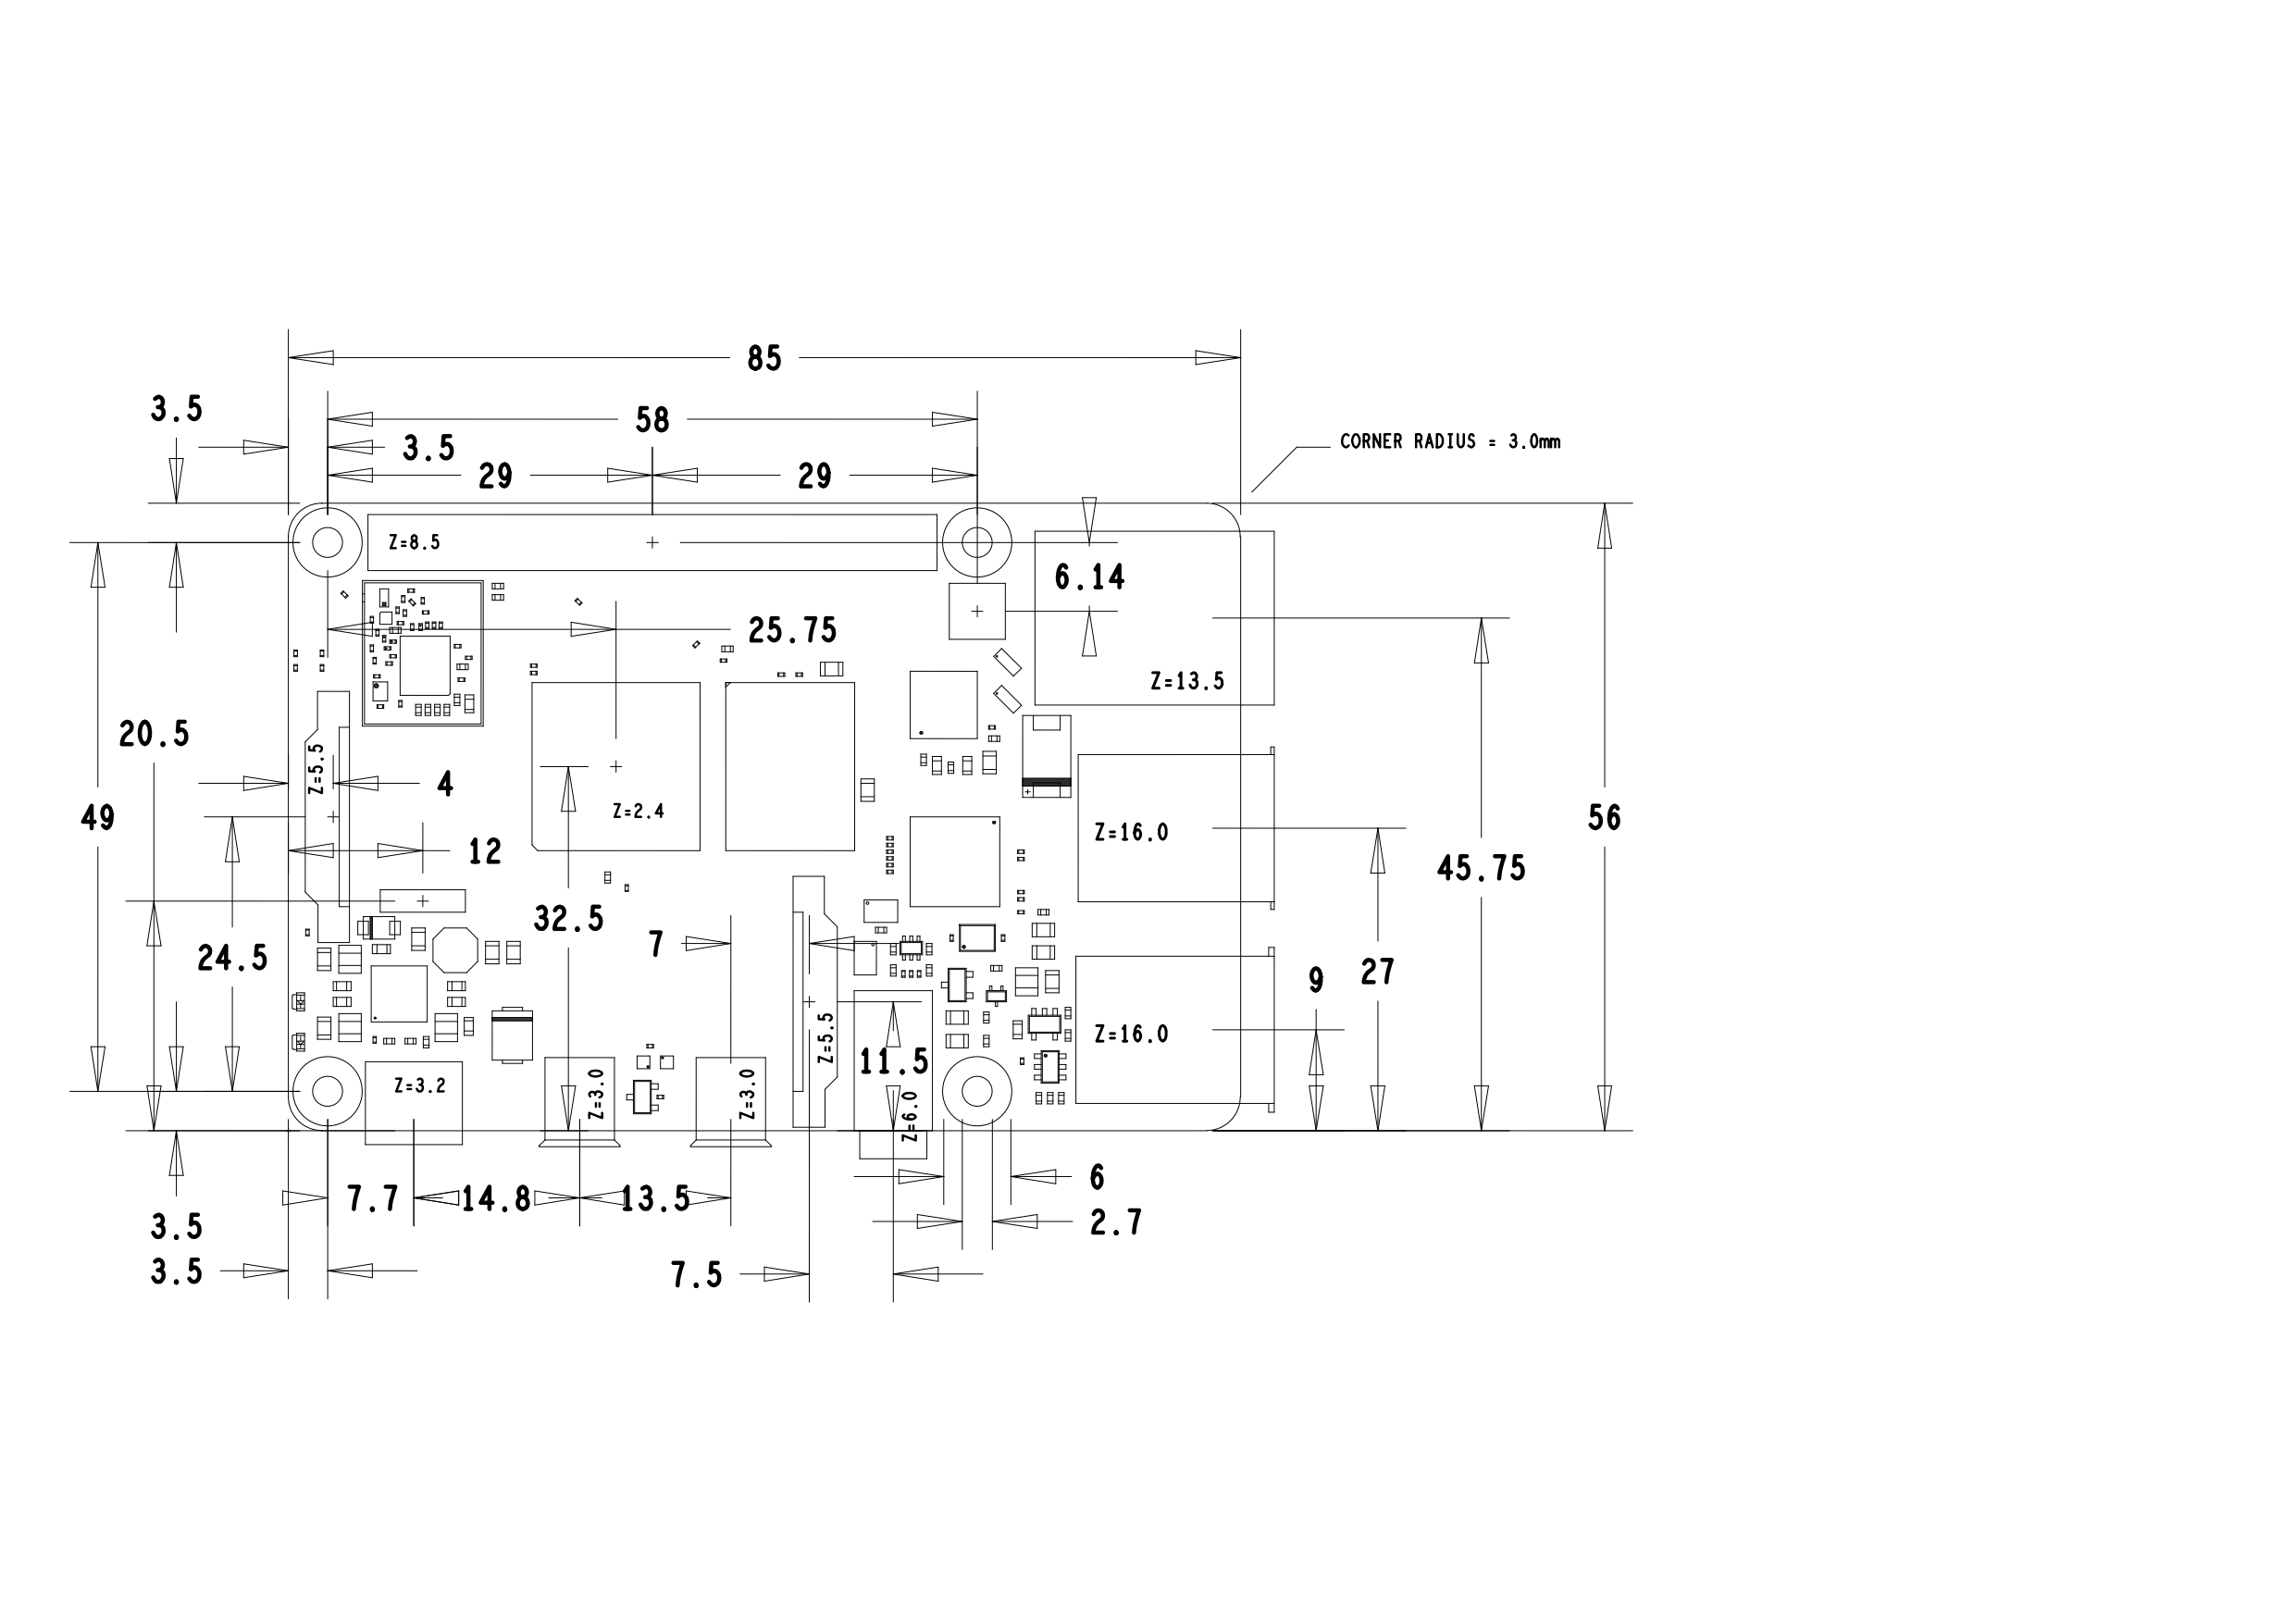
\includegraphics[width=\linewidth, angle=90]{texs/appendix/data/techspecs/pimechdraw.jpg}
    \caption{Raspberry Pi 4 Model B Mechanical Drawing}
    \label{fig:rpi-2}
\end{figure}

\subsection{Raspberry Pi Camera Module V2}

\begin{figure}[H]
    \centering
    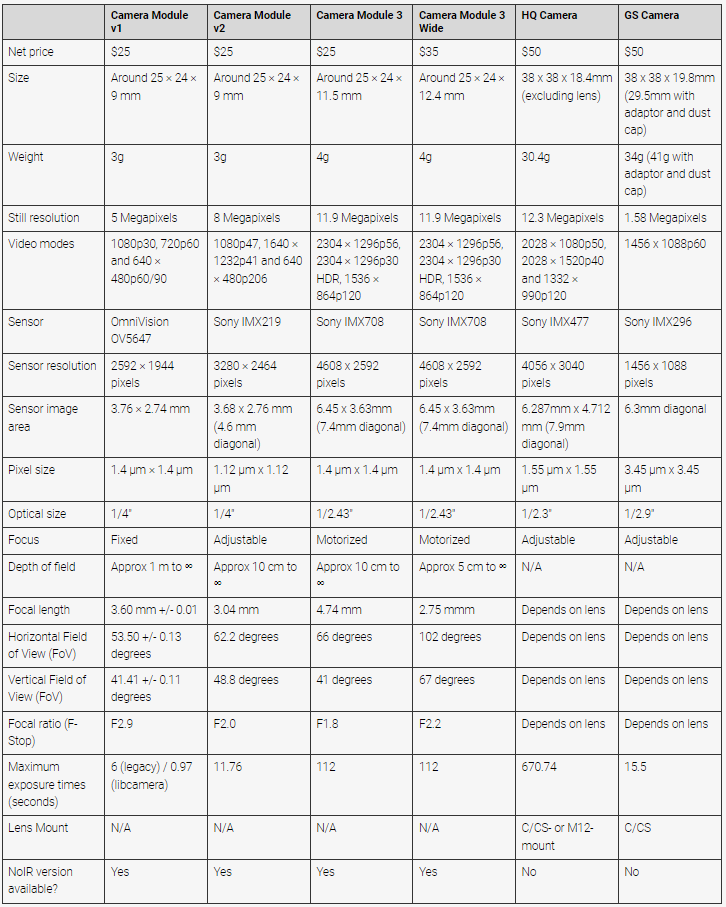
\includegraphics[width=0.85\linewidth]{texs/appendix/data/techspecs/cameraspecs.png}
    \caption{Raspberry Pi Camera Module V2 Technical Specifications}
    \label{fig:picam-1}
\end{figure}

\begin{figure}[H]
    \centering
    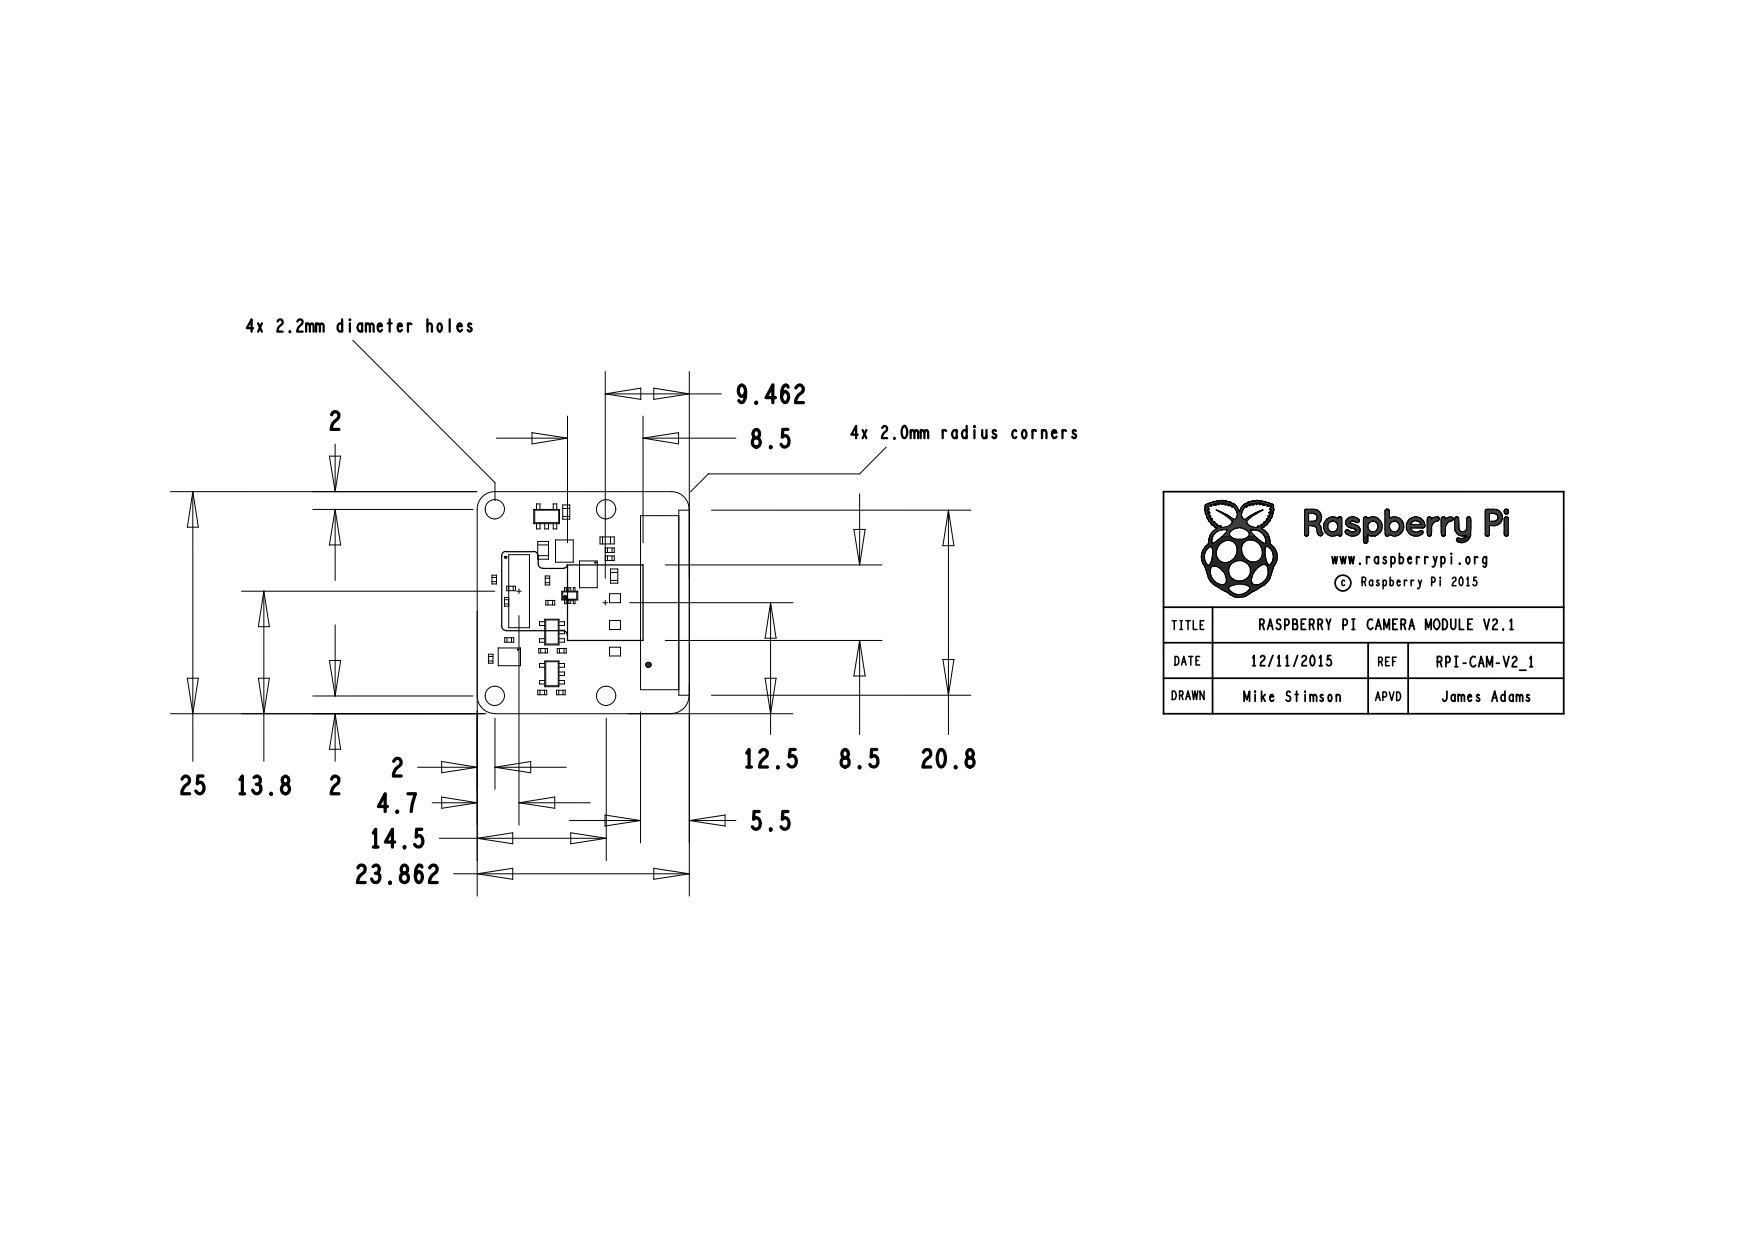
\includegraphics[width=\linewidth, angle=90]{texs/appendix/data/techspecs/cameramechdraw.jpg}
    \caption{Raspberry Pi Camera Module V2 Mechanical Drawing}
    \label{fig:picam-2}
\end{figure}

\subsection{Waveshare 7inch HDMI LCD (H)}

\begin{figure}[H]
    \centering
    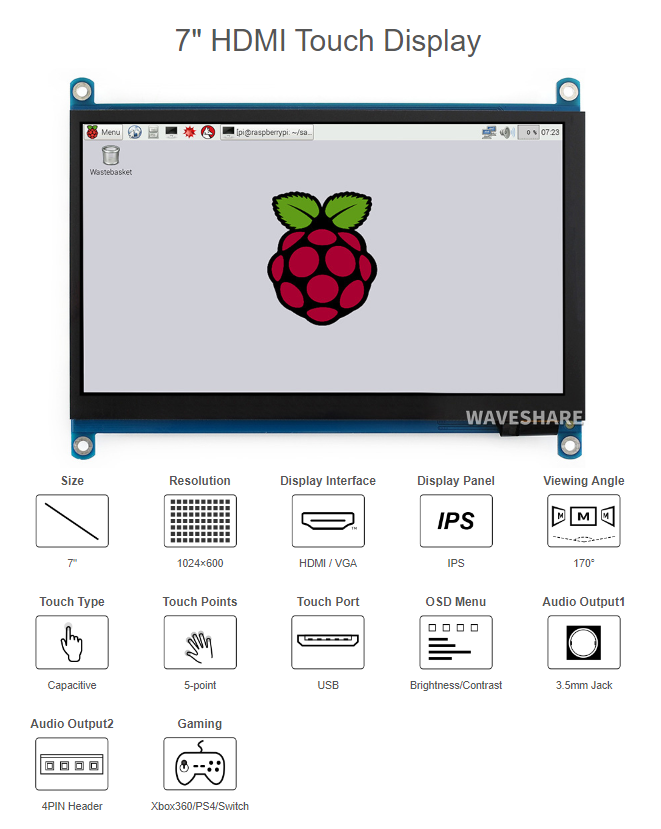
\includegraphics[width=0.85\linewidth]{texs/appendix/data/techspecs/screen1.png}
    \caption{Waveshare 7inch HDMI LCD (H) Technical Specifications -1 }
    \label{fig:lcd-1}
\end{figure}

\begin{figure}[H]
    \centering
    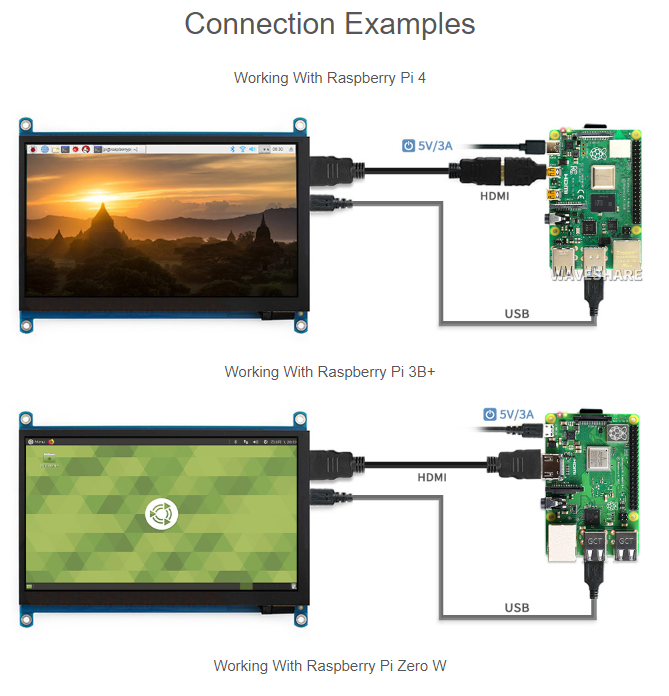
\includegraphics[width=0.85\linewidth]{texs/appendix/data/techspecs/screen2.png}
    \caption{Waveshare 7inch HDMI LCD (H) Technical Specifications -2 }
    \label{fig:lcd-2}
\end{figure}

\begin{figure}[H]
    \centering
    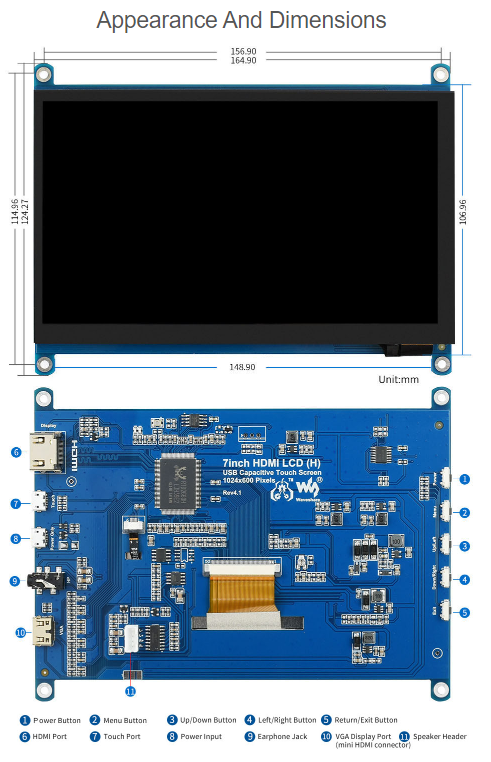
\includegraphics[width=0.85\linewidth]{texs/appendix/data/techspecs/screen3.png}
    \caption{Waveshare 7inch HDMI LCD (H) Technical Specifications -3 }
    \label{fig:lcd-3}
\end{figure}

\subsection{Veektomx VT103}

\begin{figure}[H]
    \centering
    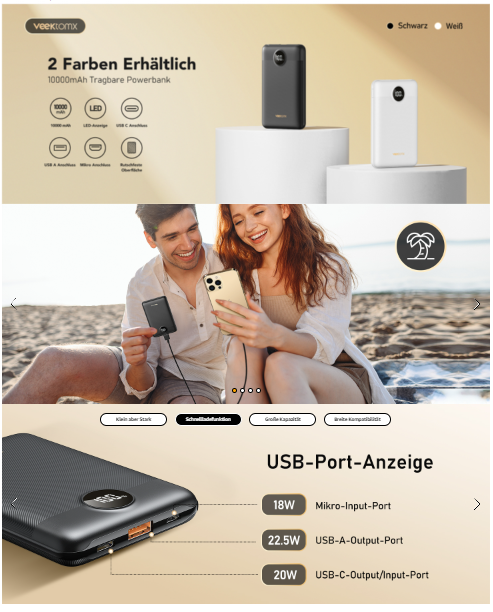
\includegraphics[width=0.85\linewidth]{texs/appendix/data/techspecs/battspecs.png}
    \caption{Veektomx VT103 Technical Specifications }
    \label{fig:battery-1}
\end{figure}

\begin{figure}[H]
    \centering
    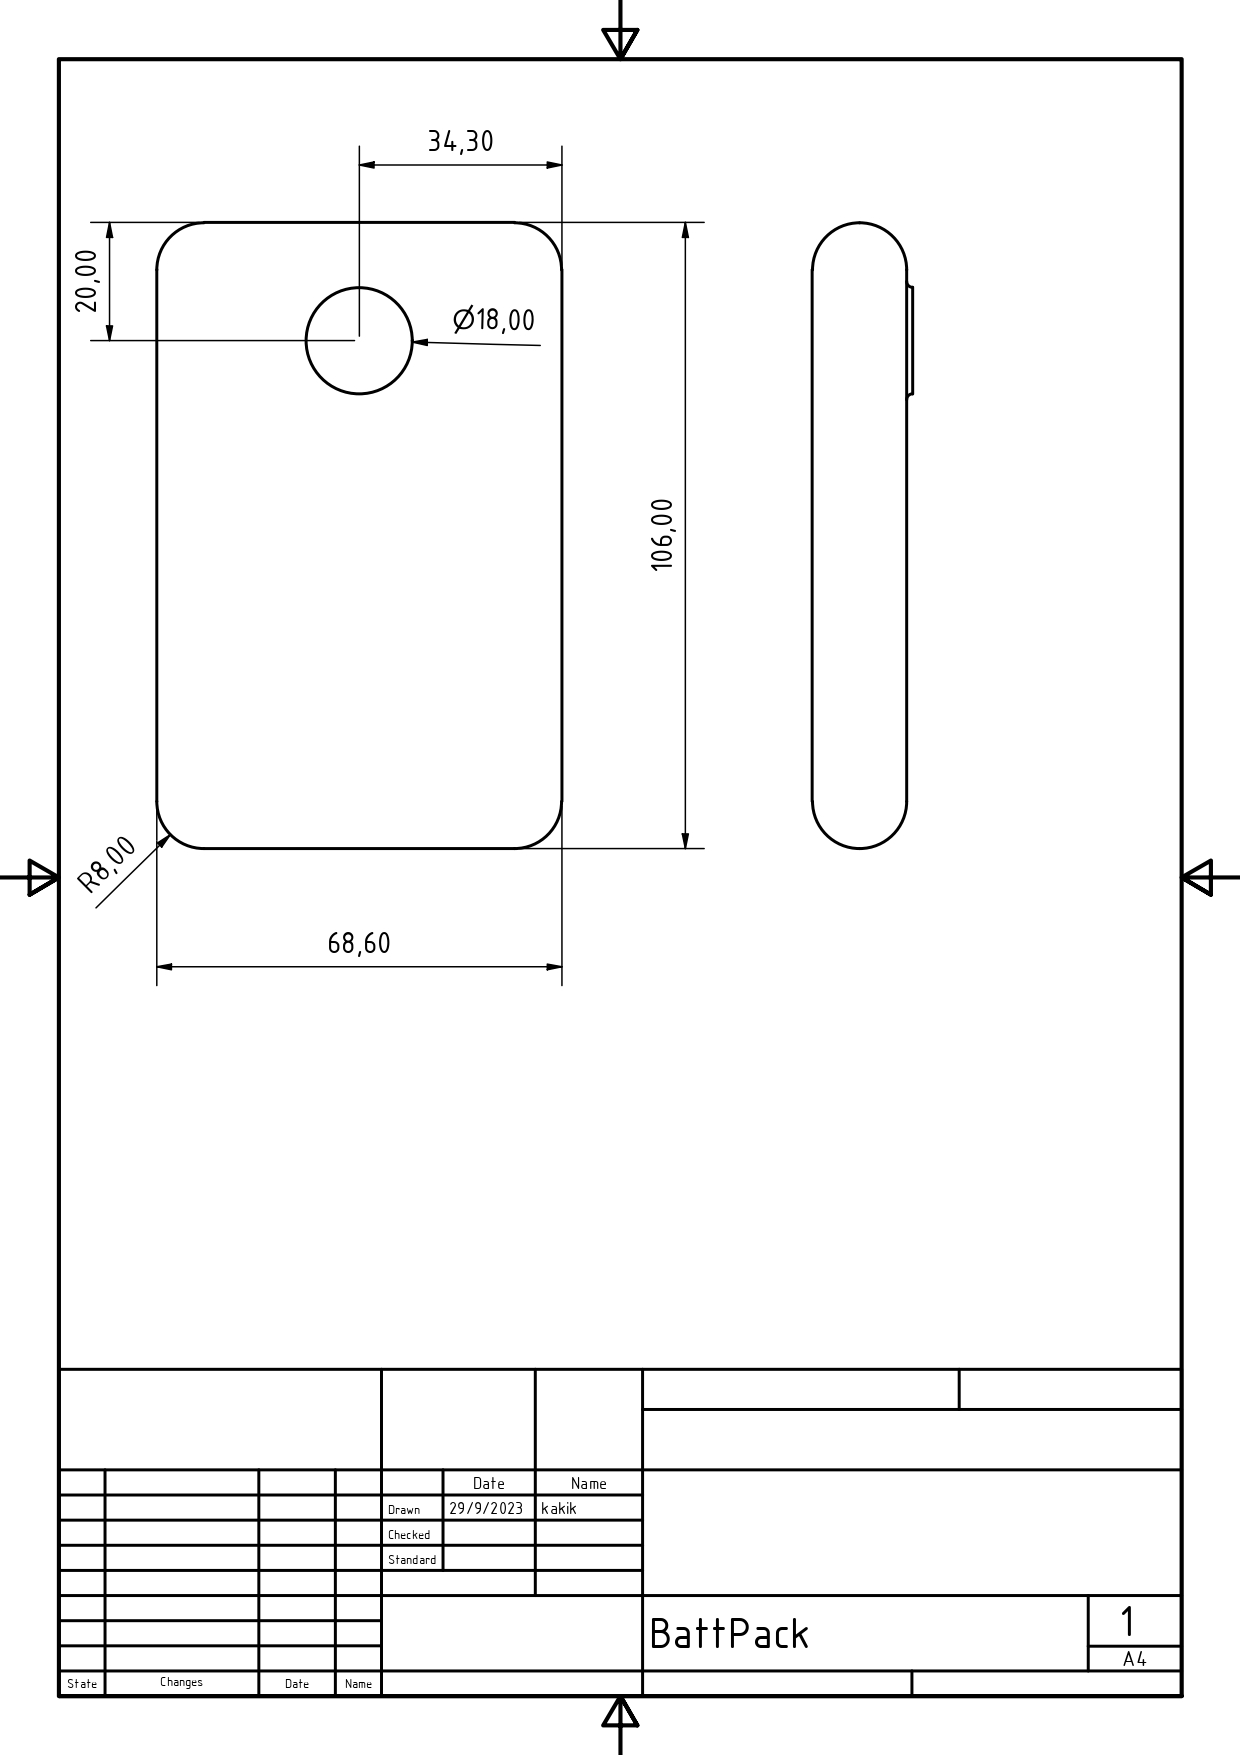
\includegraphics[width=0.85\linewidth]{texs/appendix/data/techspecs/battmechdraw.jpg}
    \caption{Veektomx VT103 Mechanical Drawing }
    \label{fig:battery-2}
\end{figure}

\subsection{Ruthex Brass Inserts}

\begin{figure}[H]
    \centering
    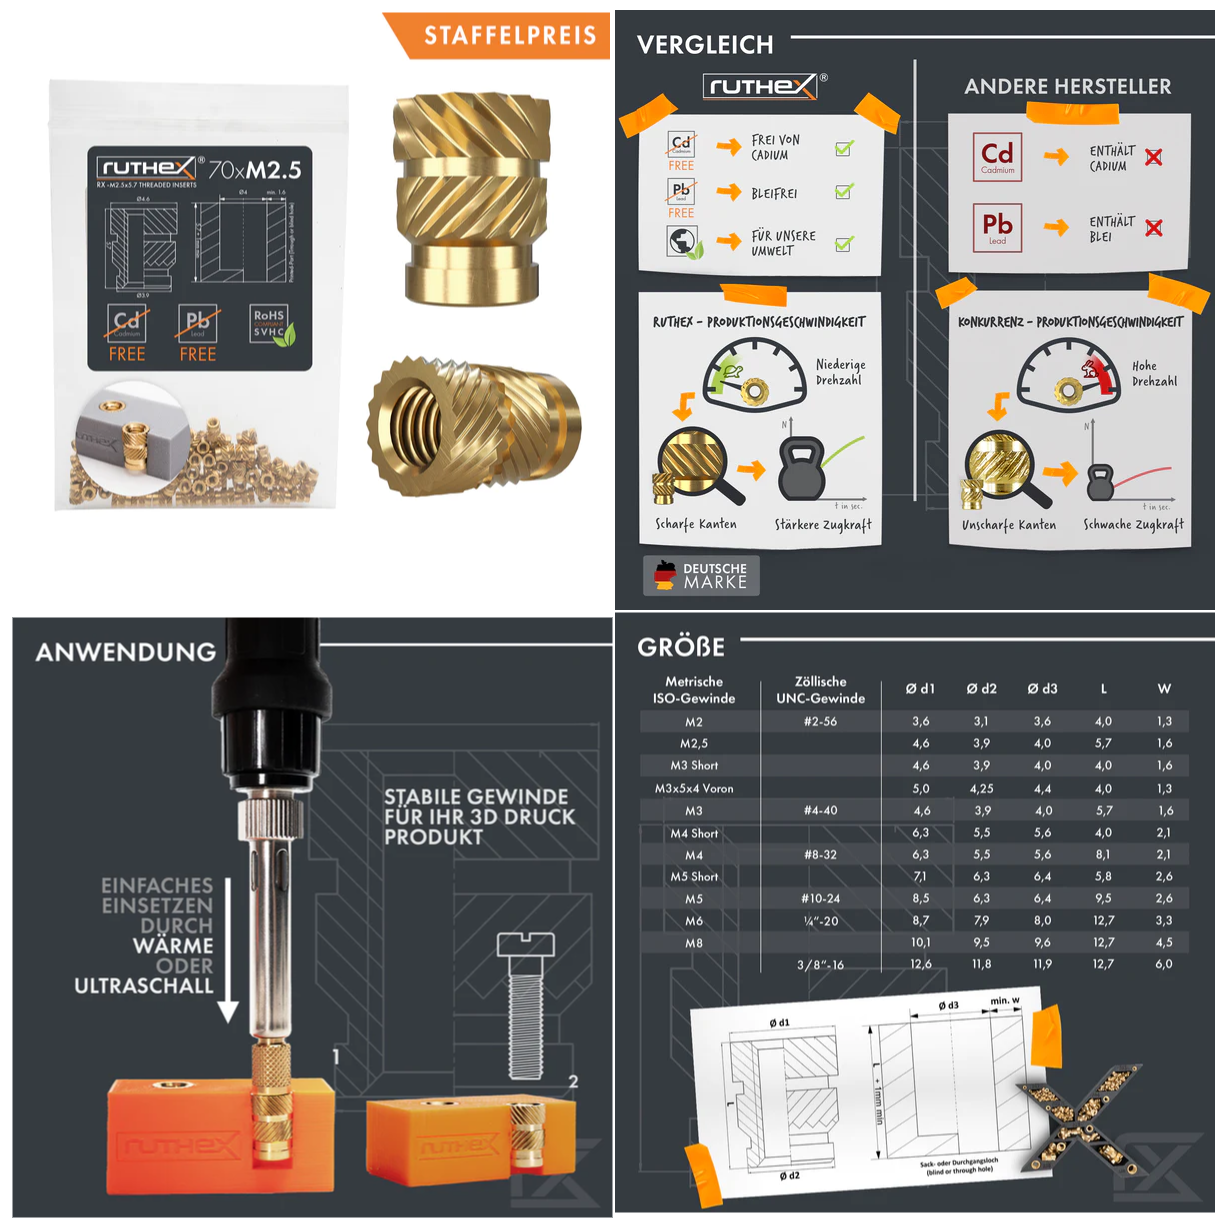
\includegraphics[width=0.85\linewidth]{texs/appendix/data/techspecs/ruthex.png}
    \caption{Ruthex Brass Inserts}
    \label{fig:insert-1}
\end{figure}

\section{Cost Calculation}
\label{appendix:cost-calculation}

\begin{figure}[H]
    \centering
    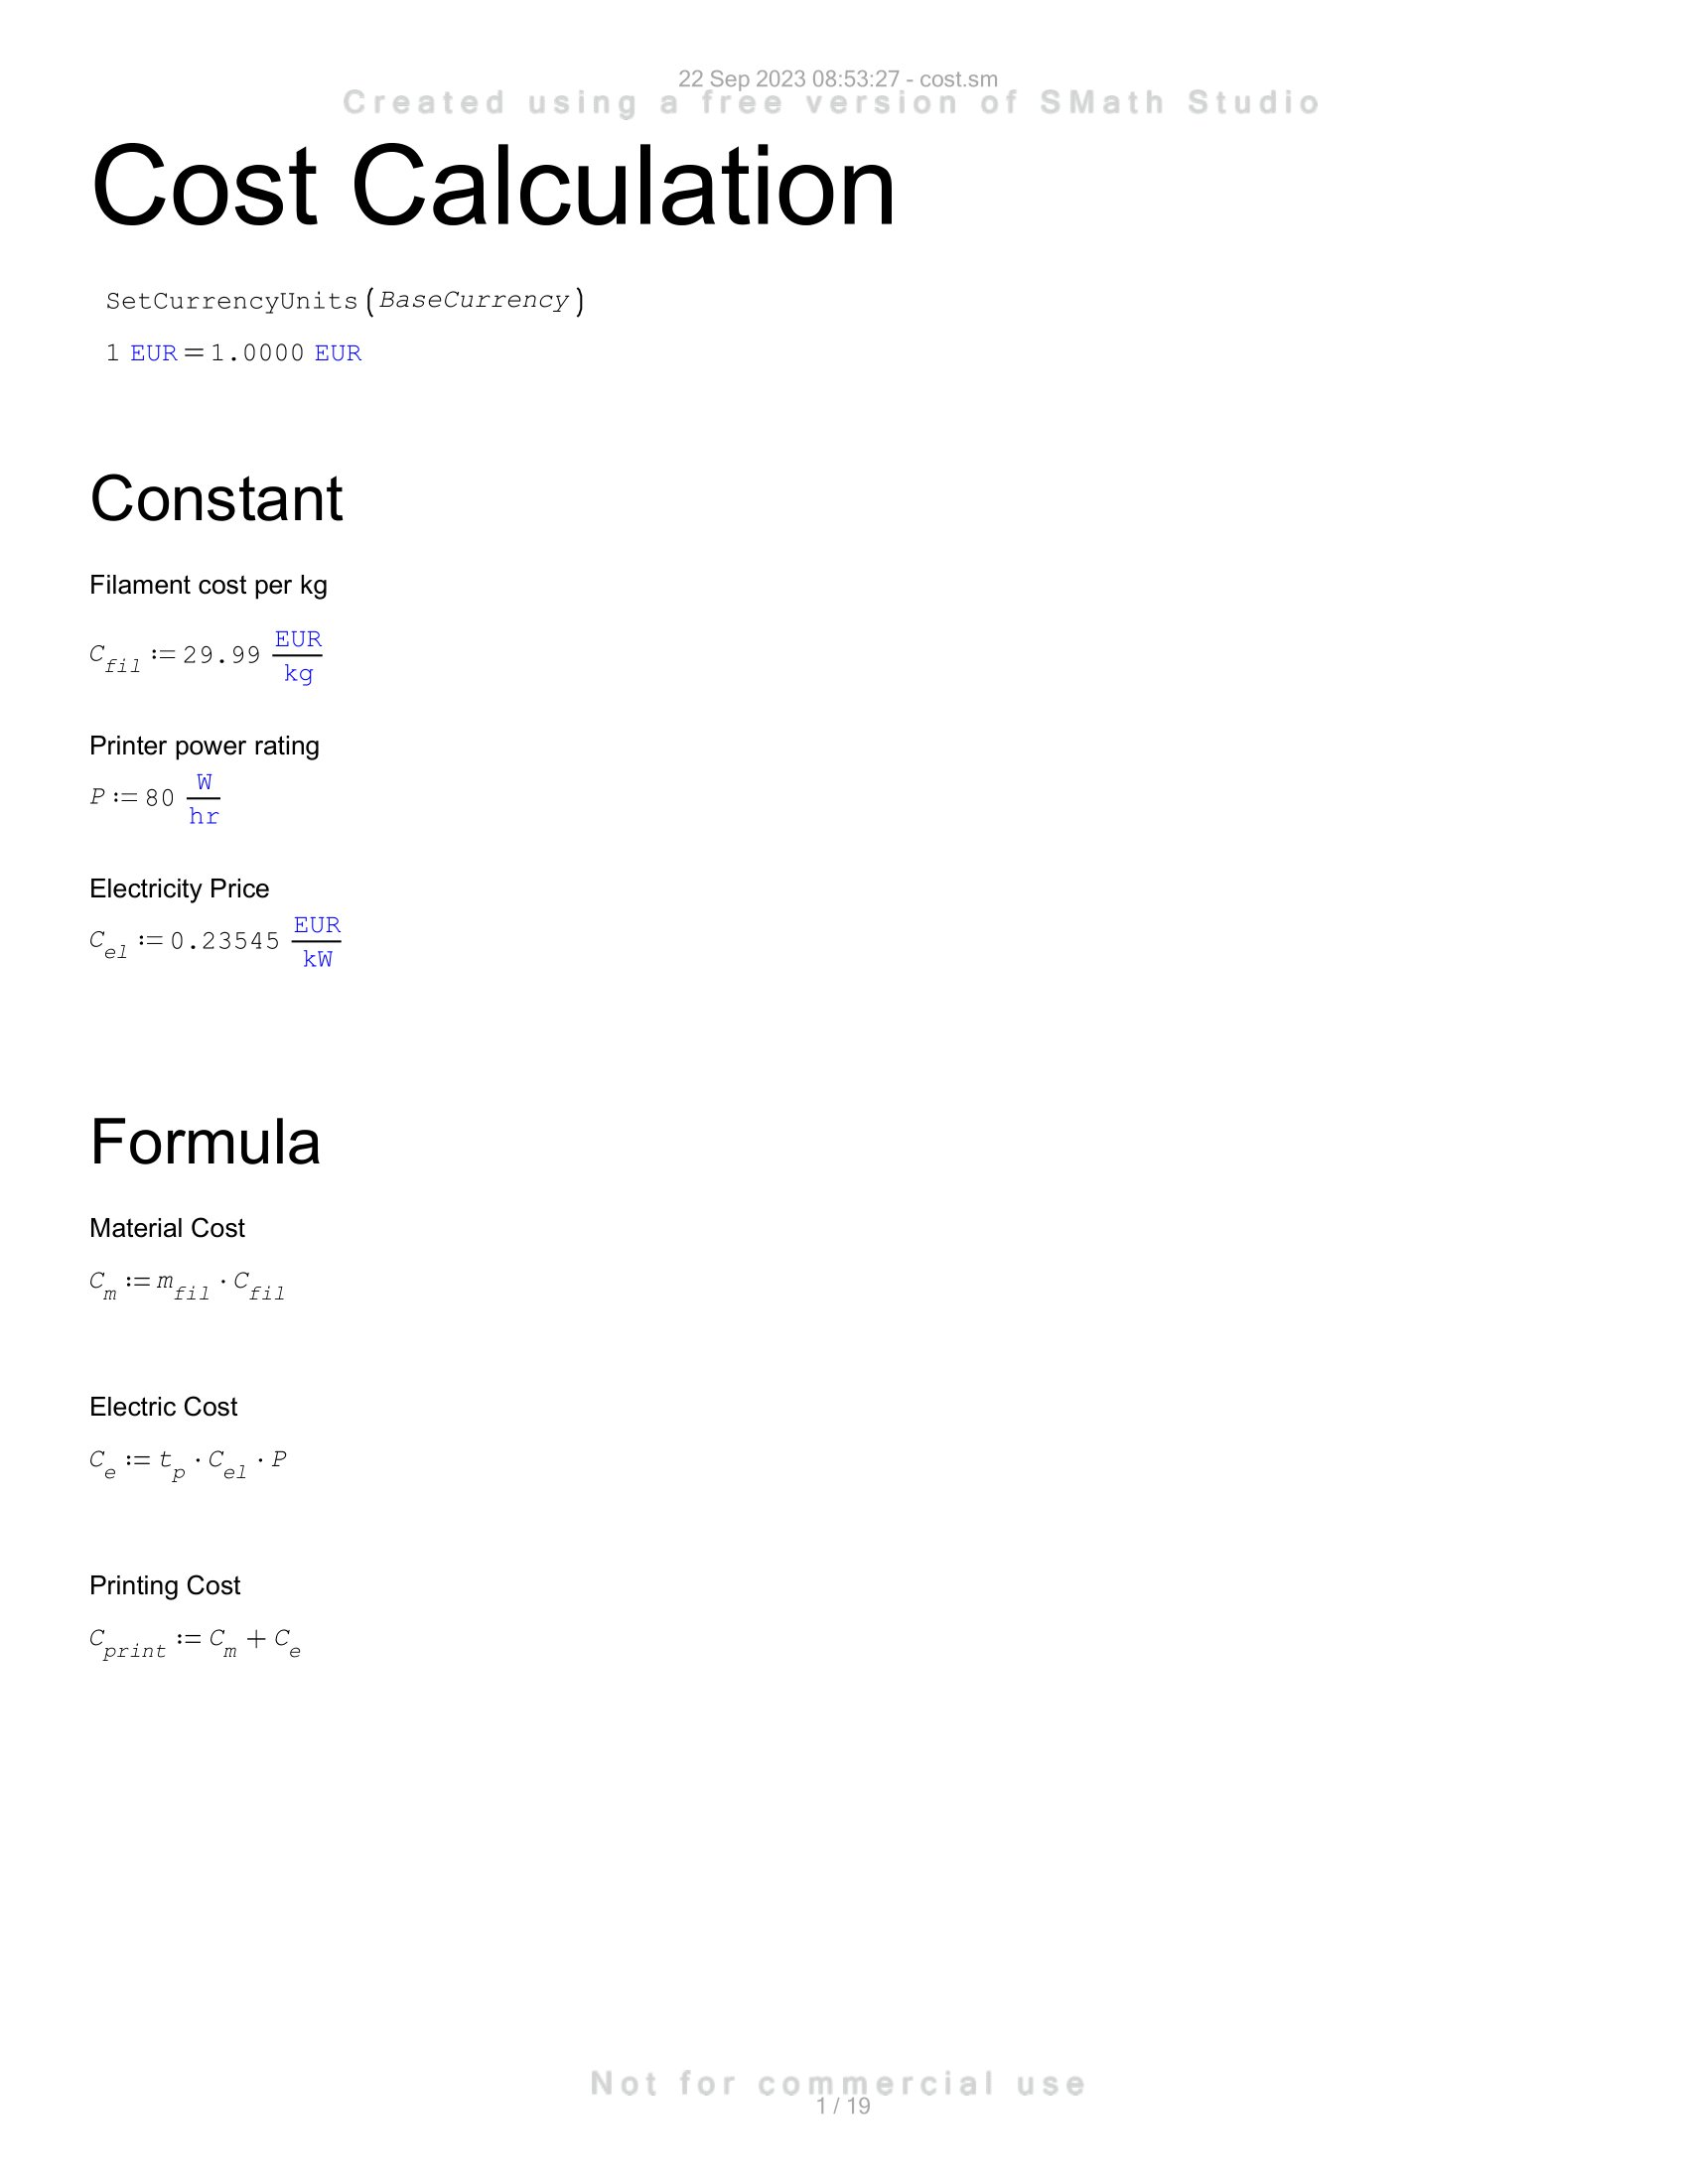
\includegraphics[width=\linewidth]{texs/appendix/data/costcalculation/cost1-01.jpg}
    \caption{Cost Calculation 1}
    \label{fig:cost-calculation-1}
\end{figure}

\begin{figure}[H]
    \centering
    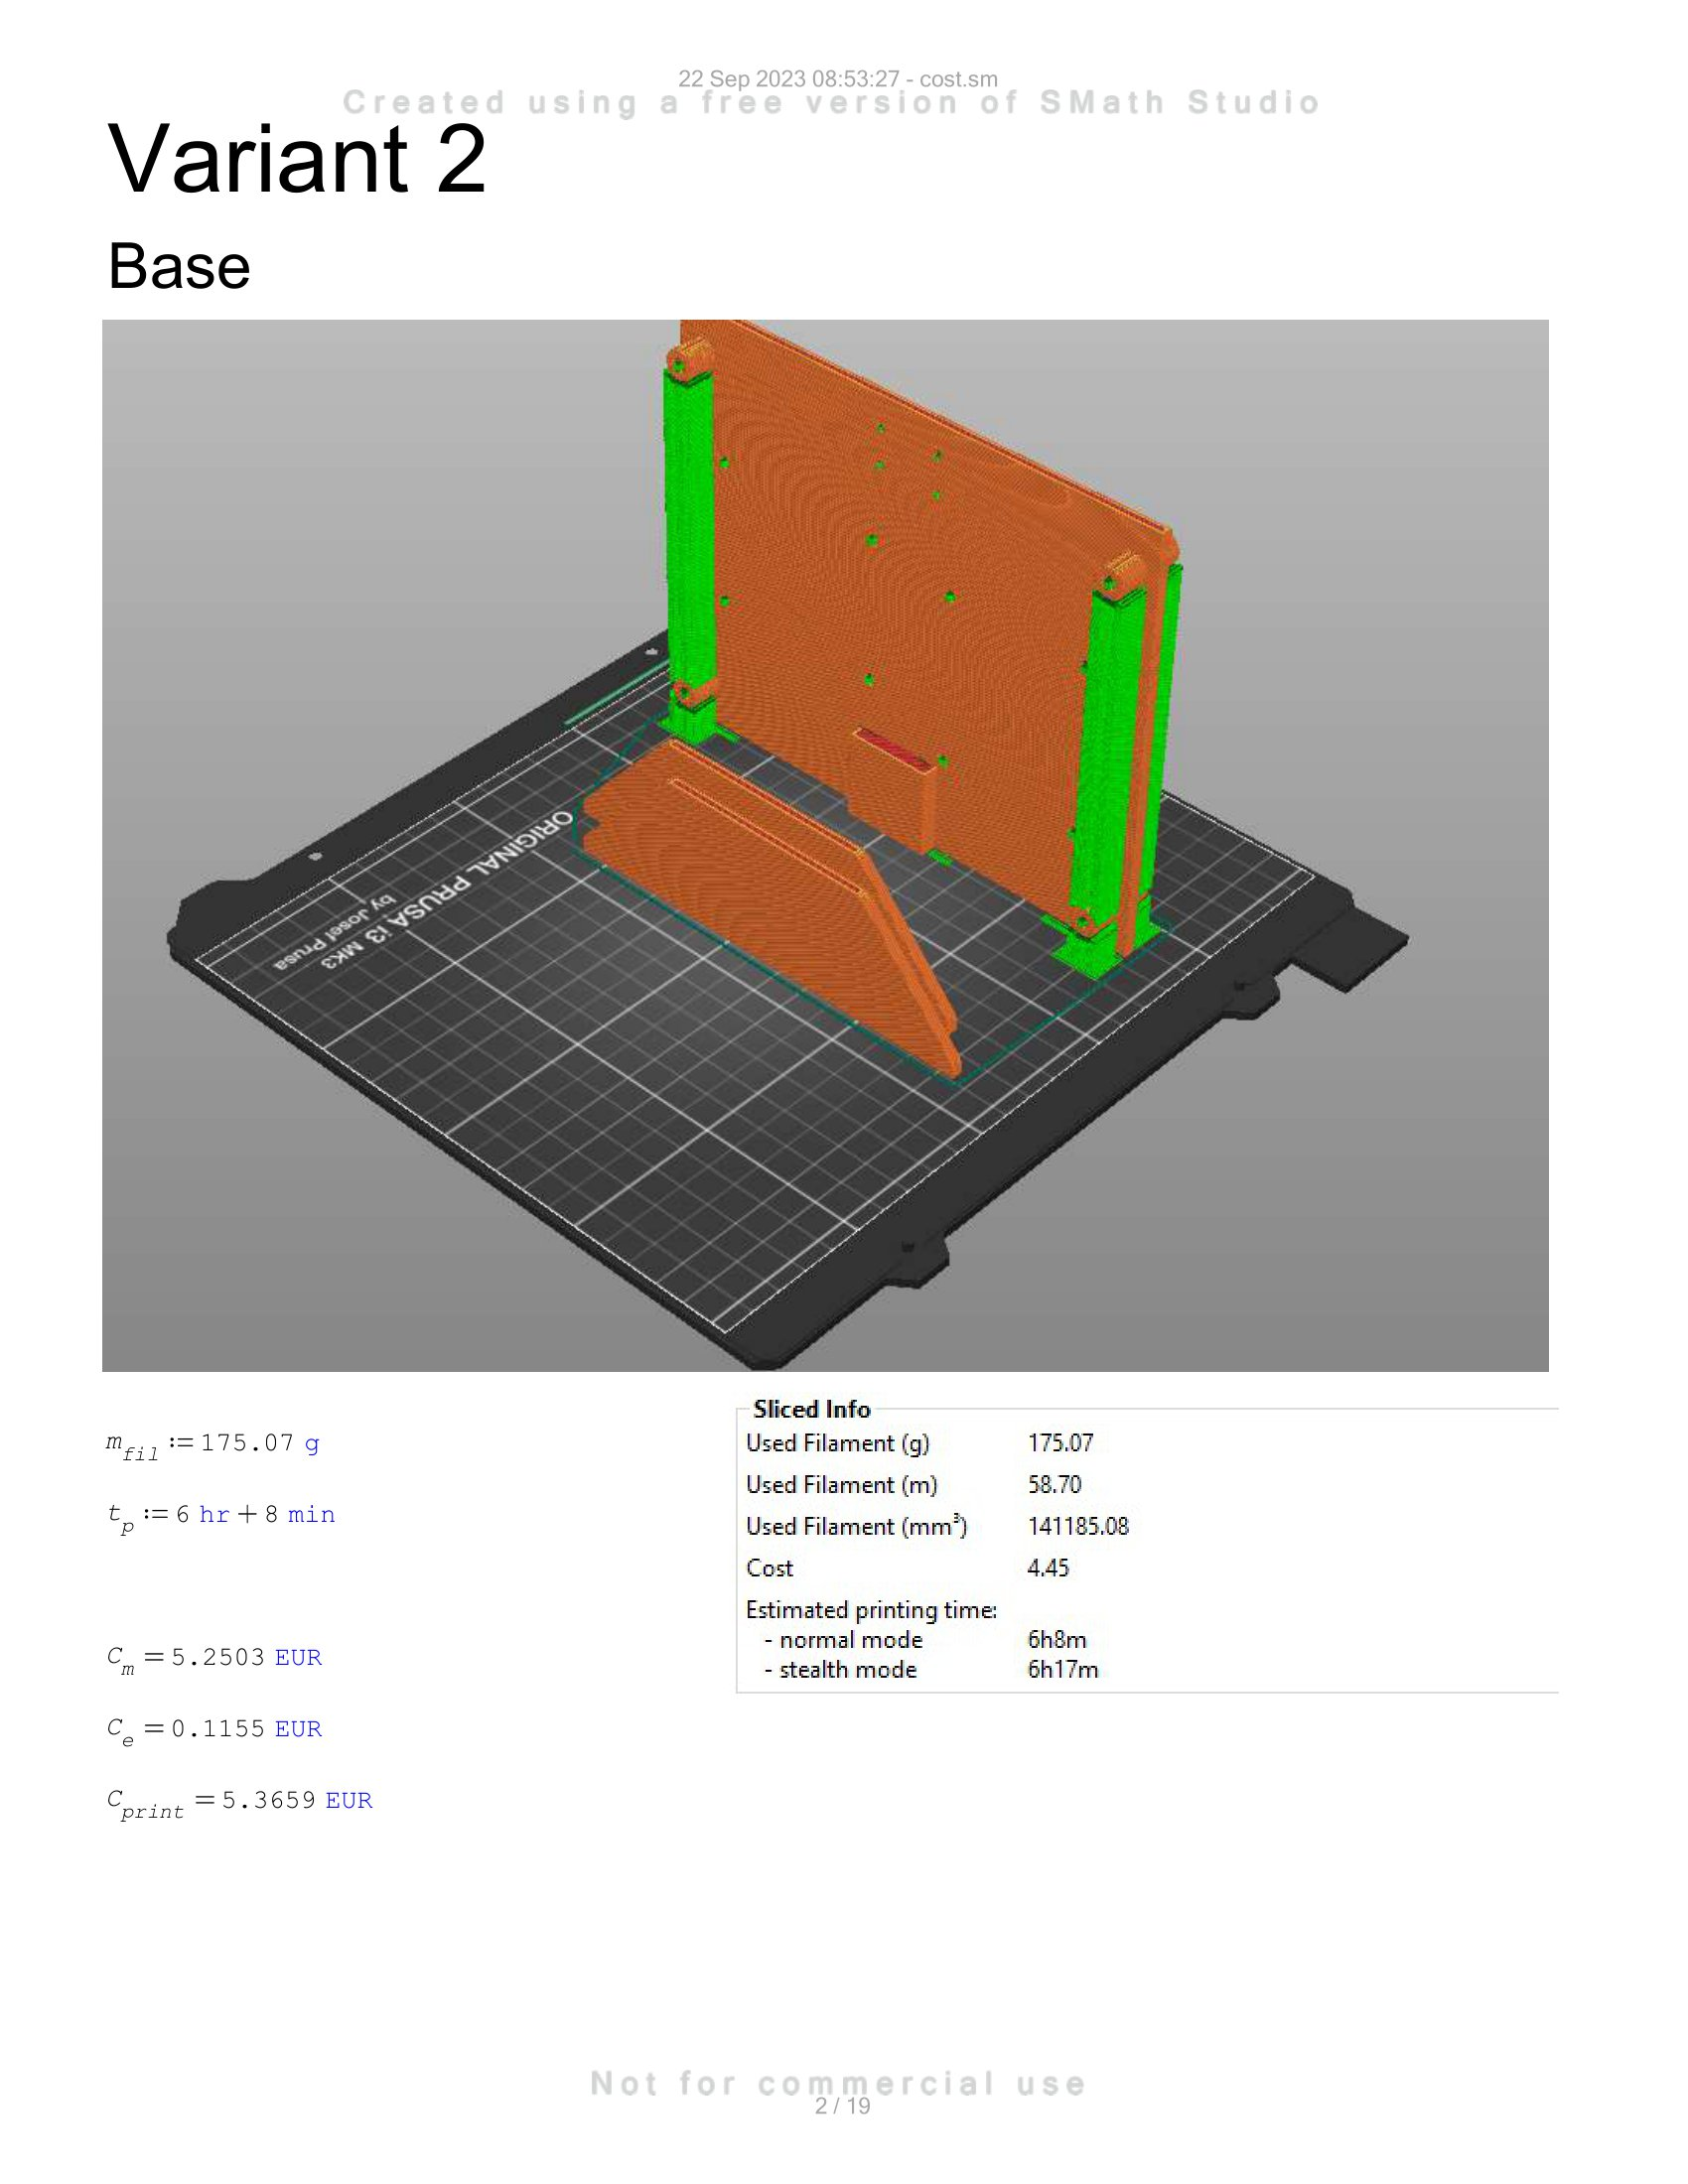
\includegraphics[width=\linewidth]{texs/appendix/data/costcalculation/cost1-02.jpg}
    \caption{Cost Calculation 2}
    \label{fig:cost-calculation-2}
\end{figure}

\begin{figure}[H]
    \centering
    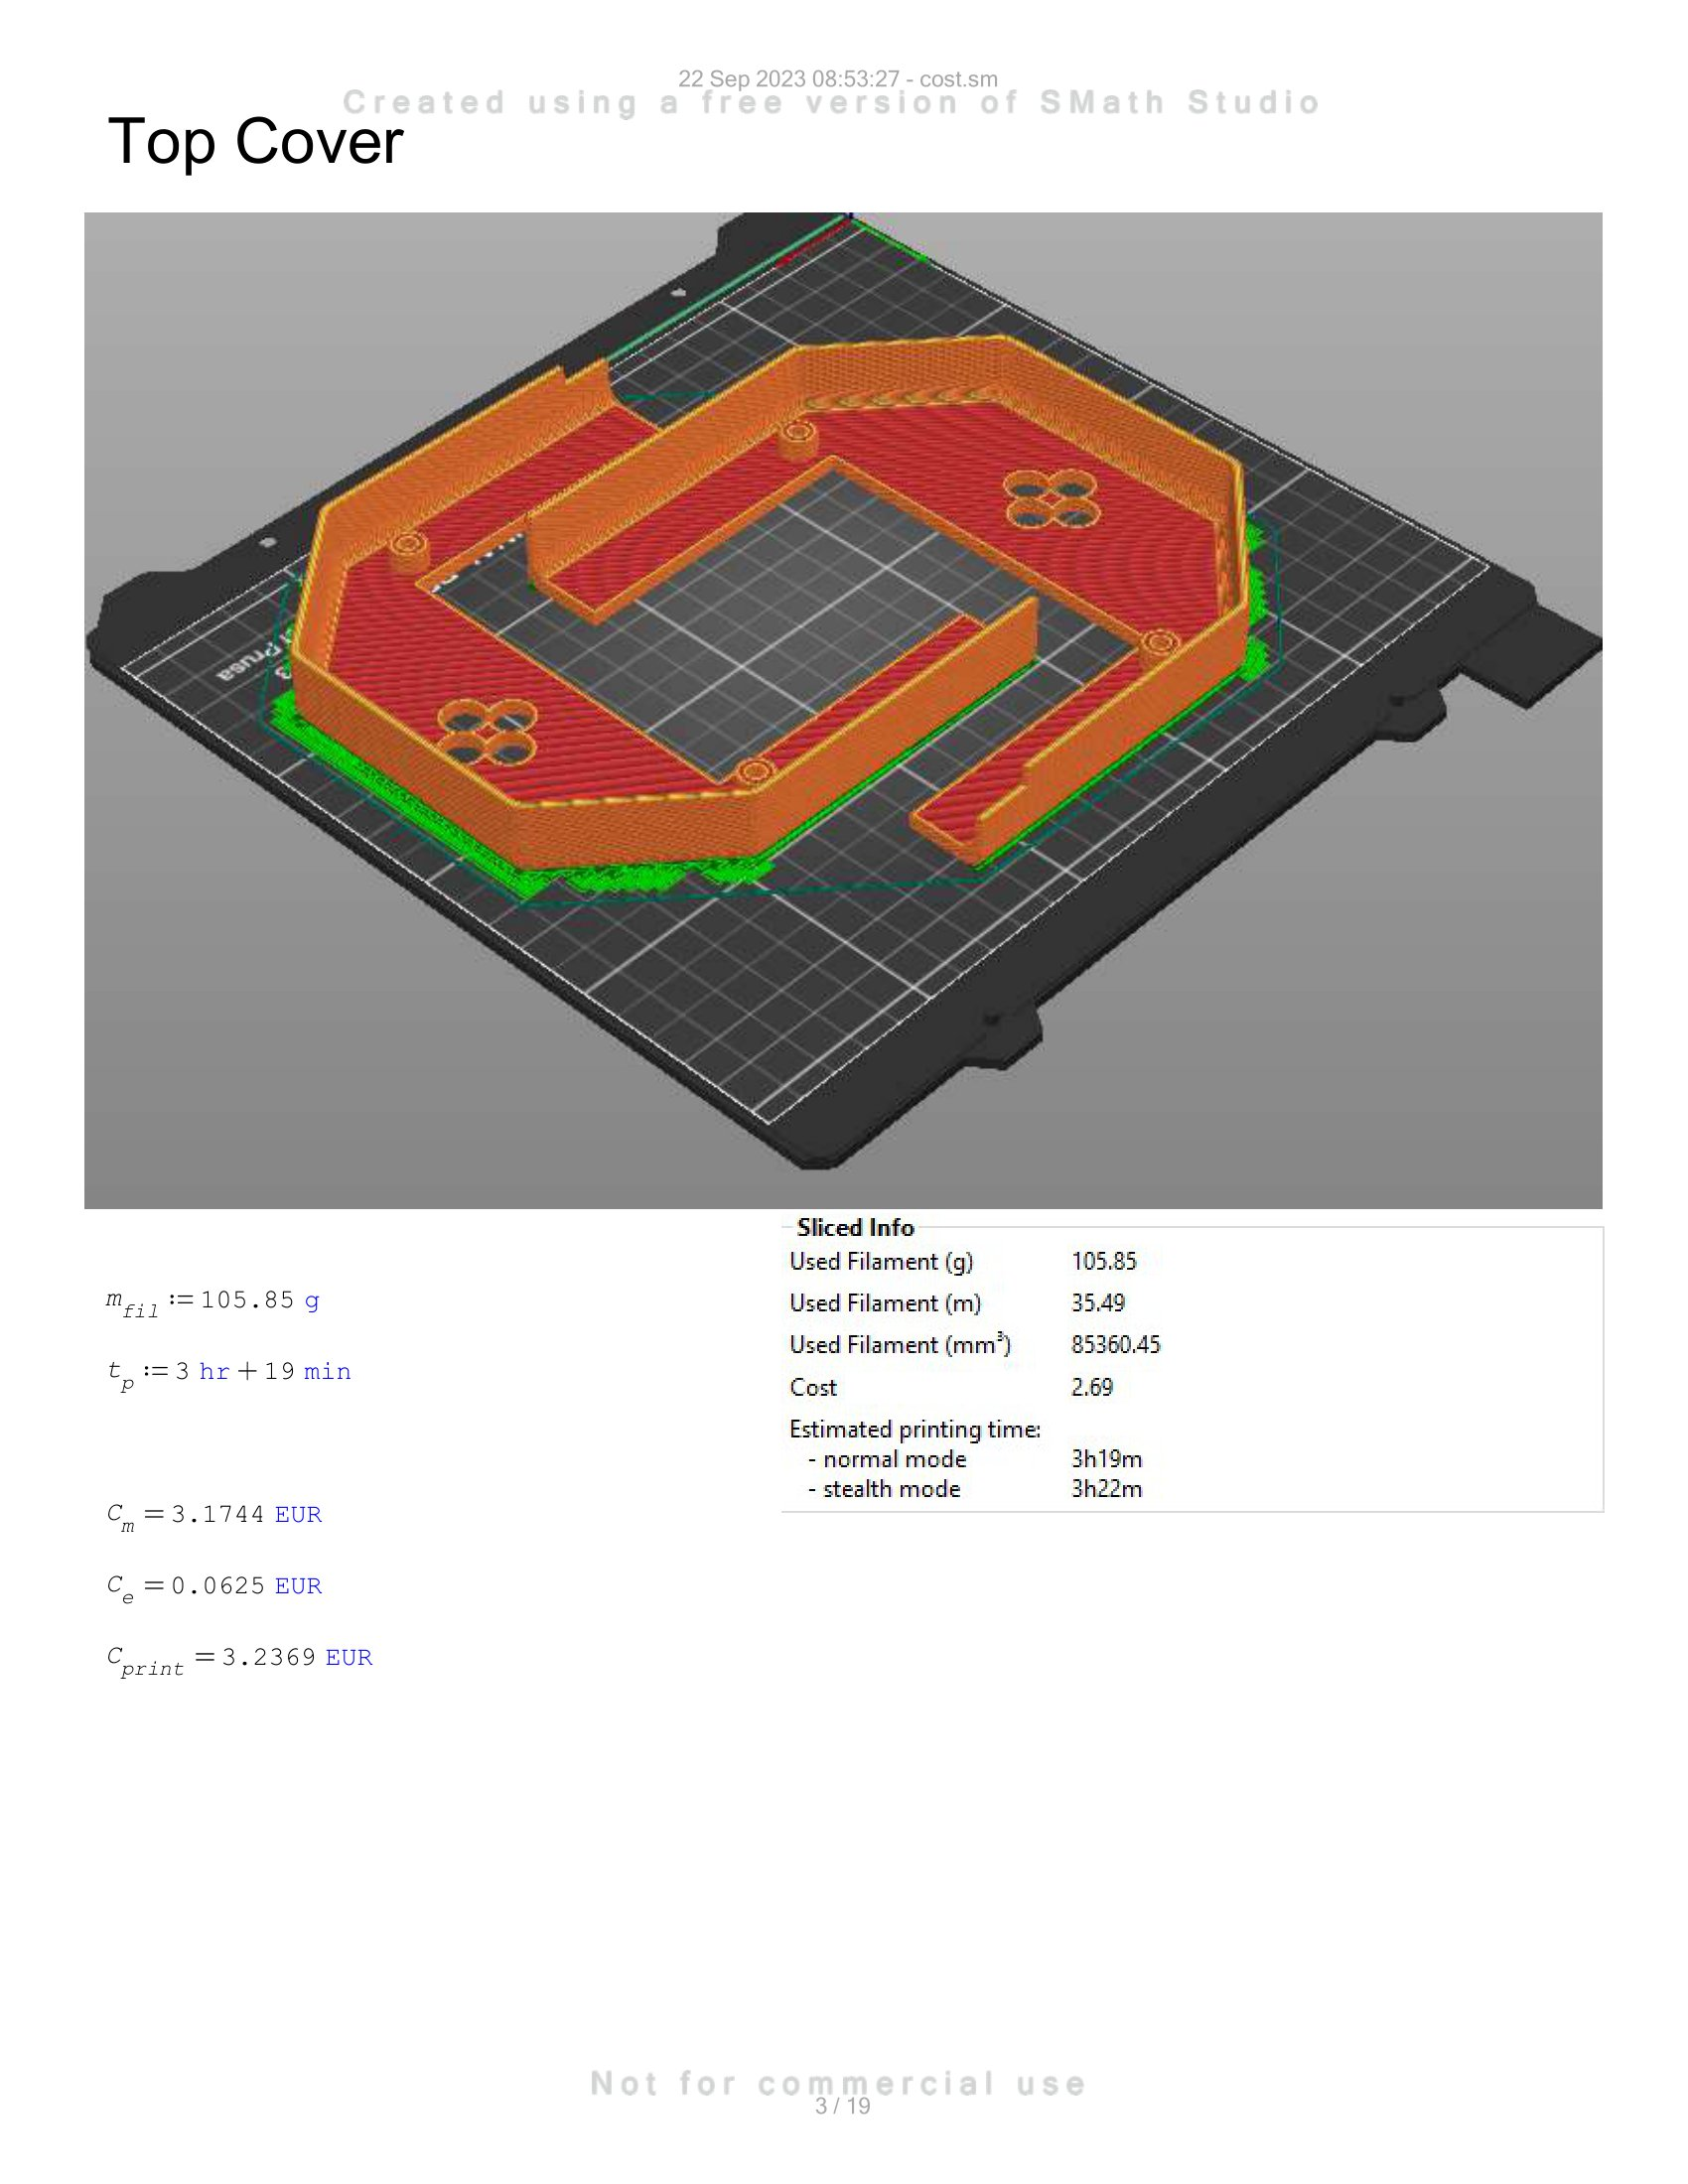
\includegraphics[width=\linewidth]{texs/appendix/data/costcalculation/cost1-03.jpg}
    \caption{Cost Calculation 3}
    \label{fig:cost-calculation-3}
\end{figure}

\begin{figure}[H]
    \centering
    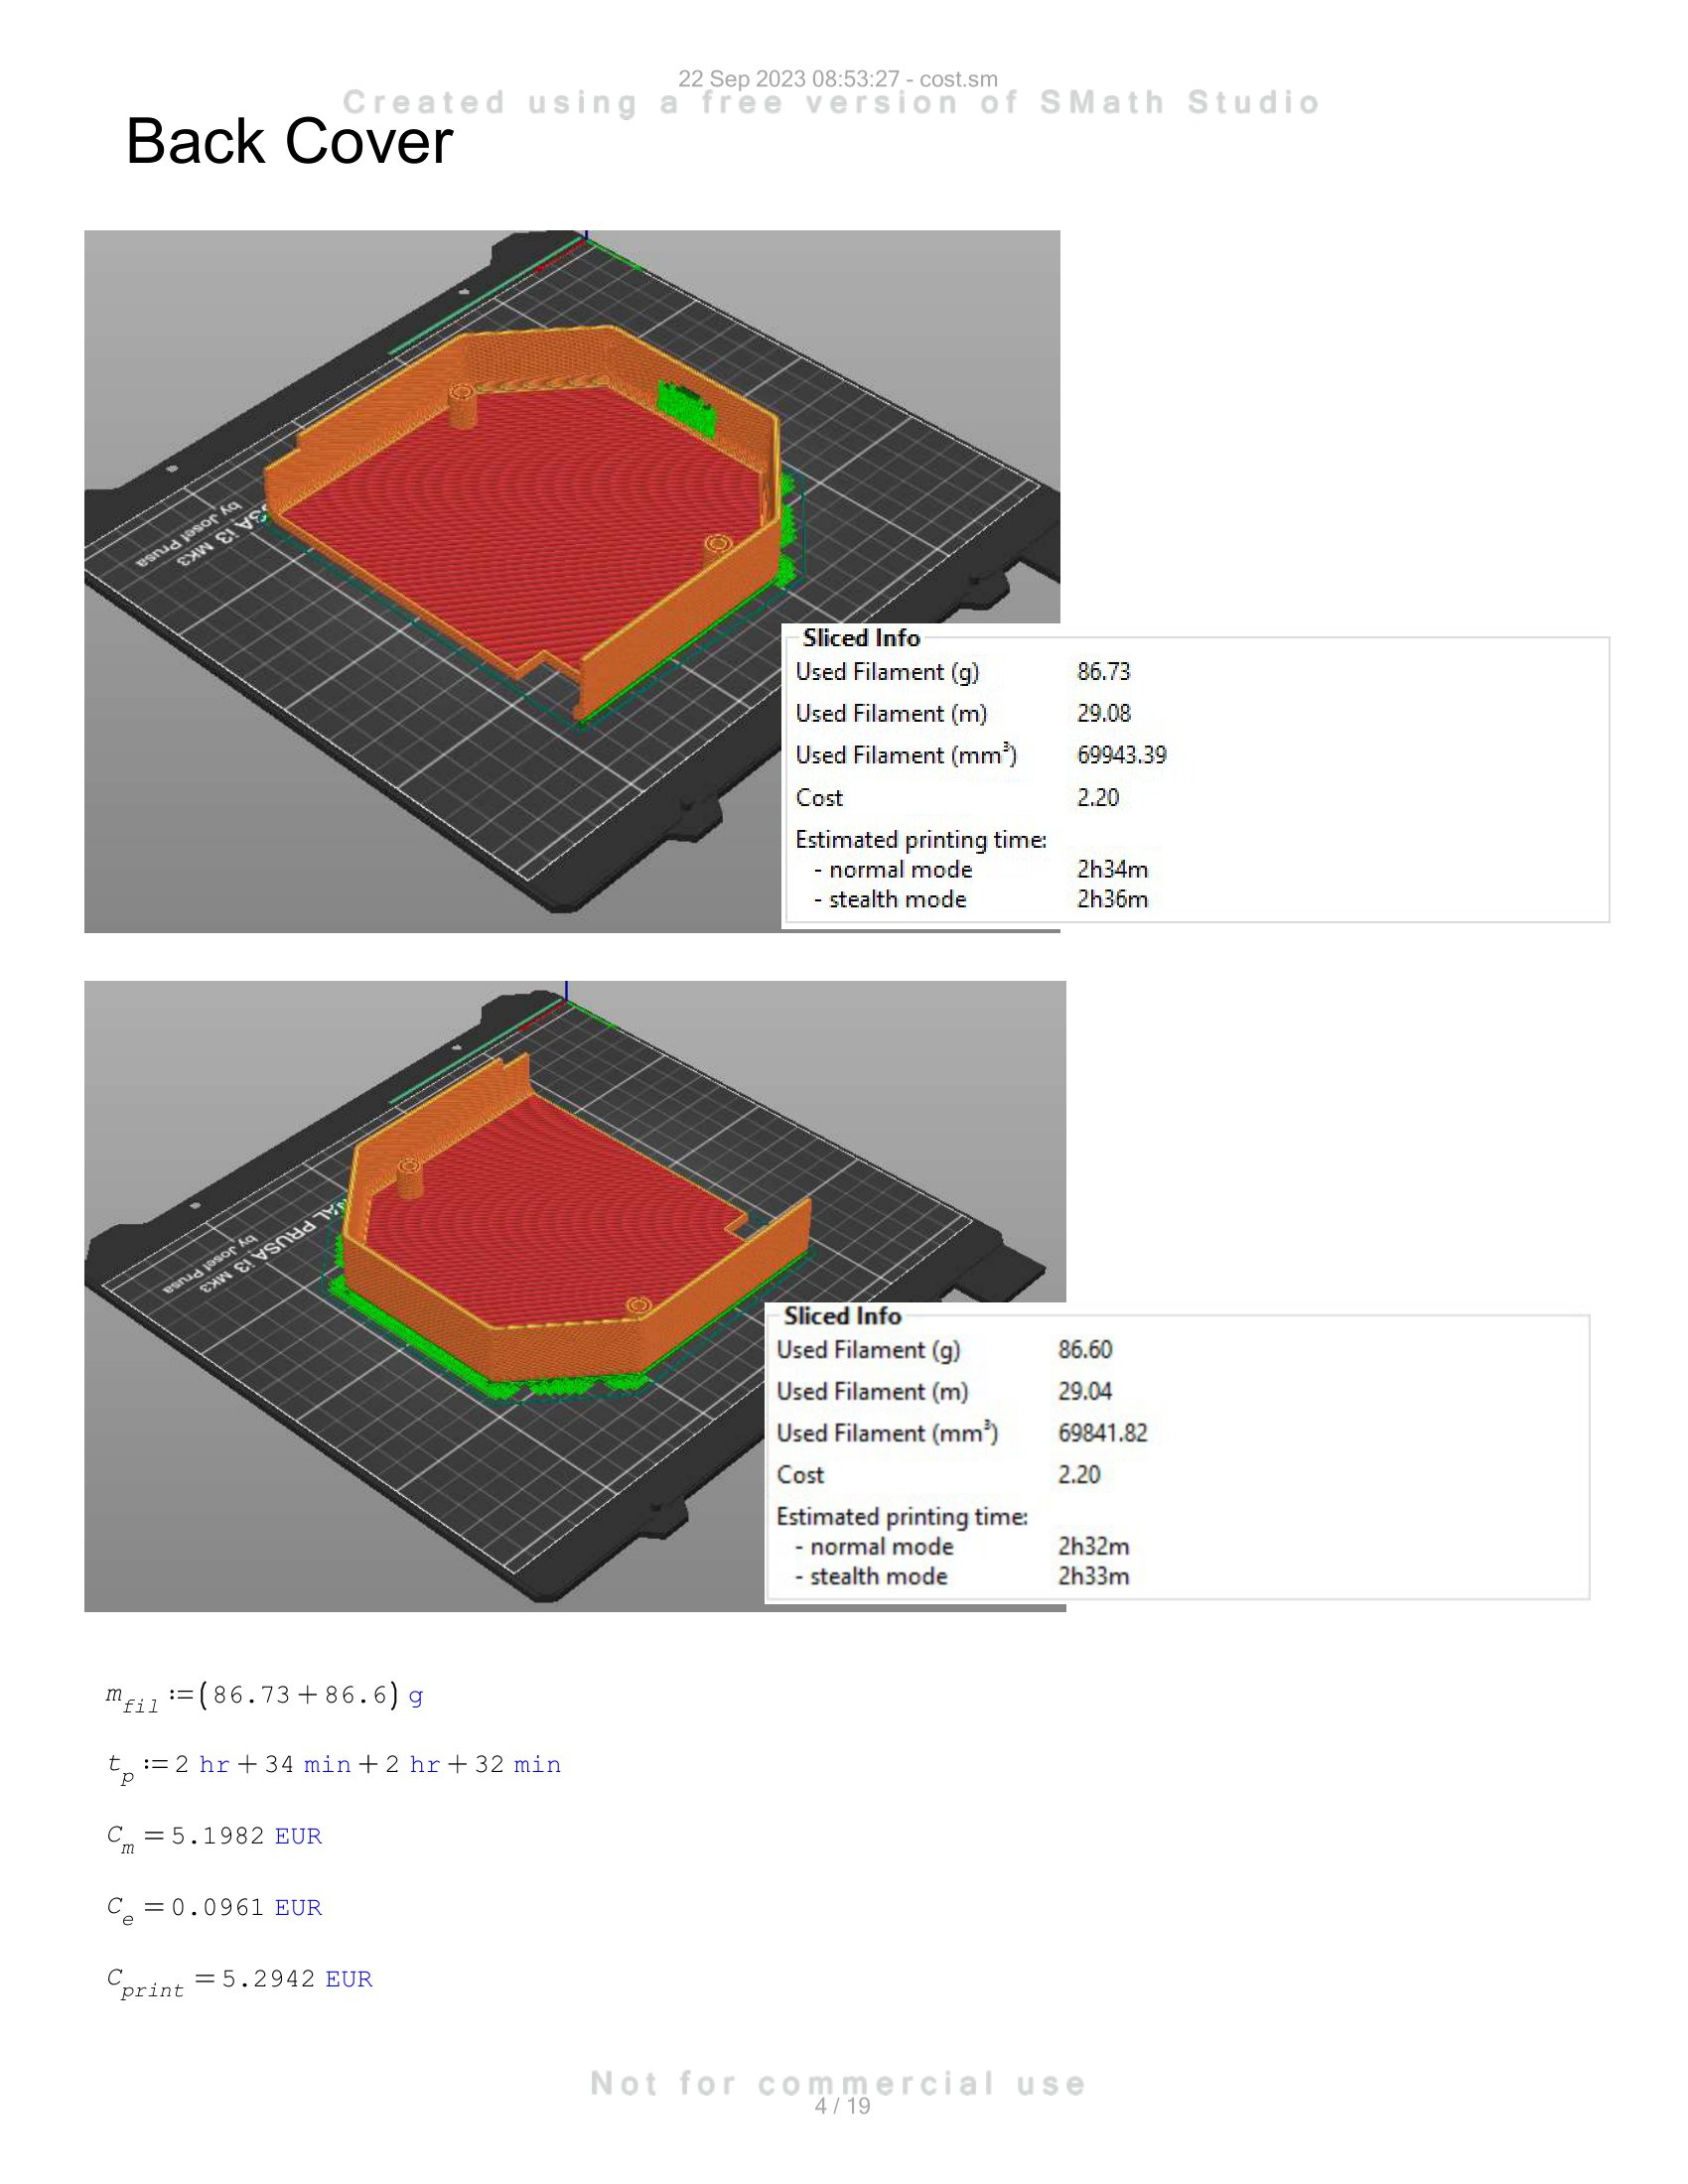
\includegraphics[width=\linewidth]{texs/appendix/data/costcalculation/cost1-04.jpg}
    \caption{Cost Calculation 4}
    \label{fig:cost-calculation-4}
\end{figure}

\begin{figure}[H]
    \centering
    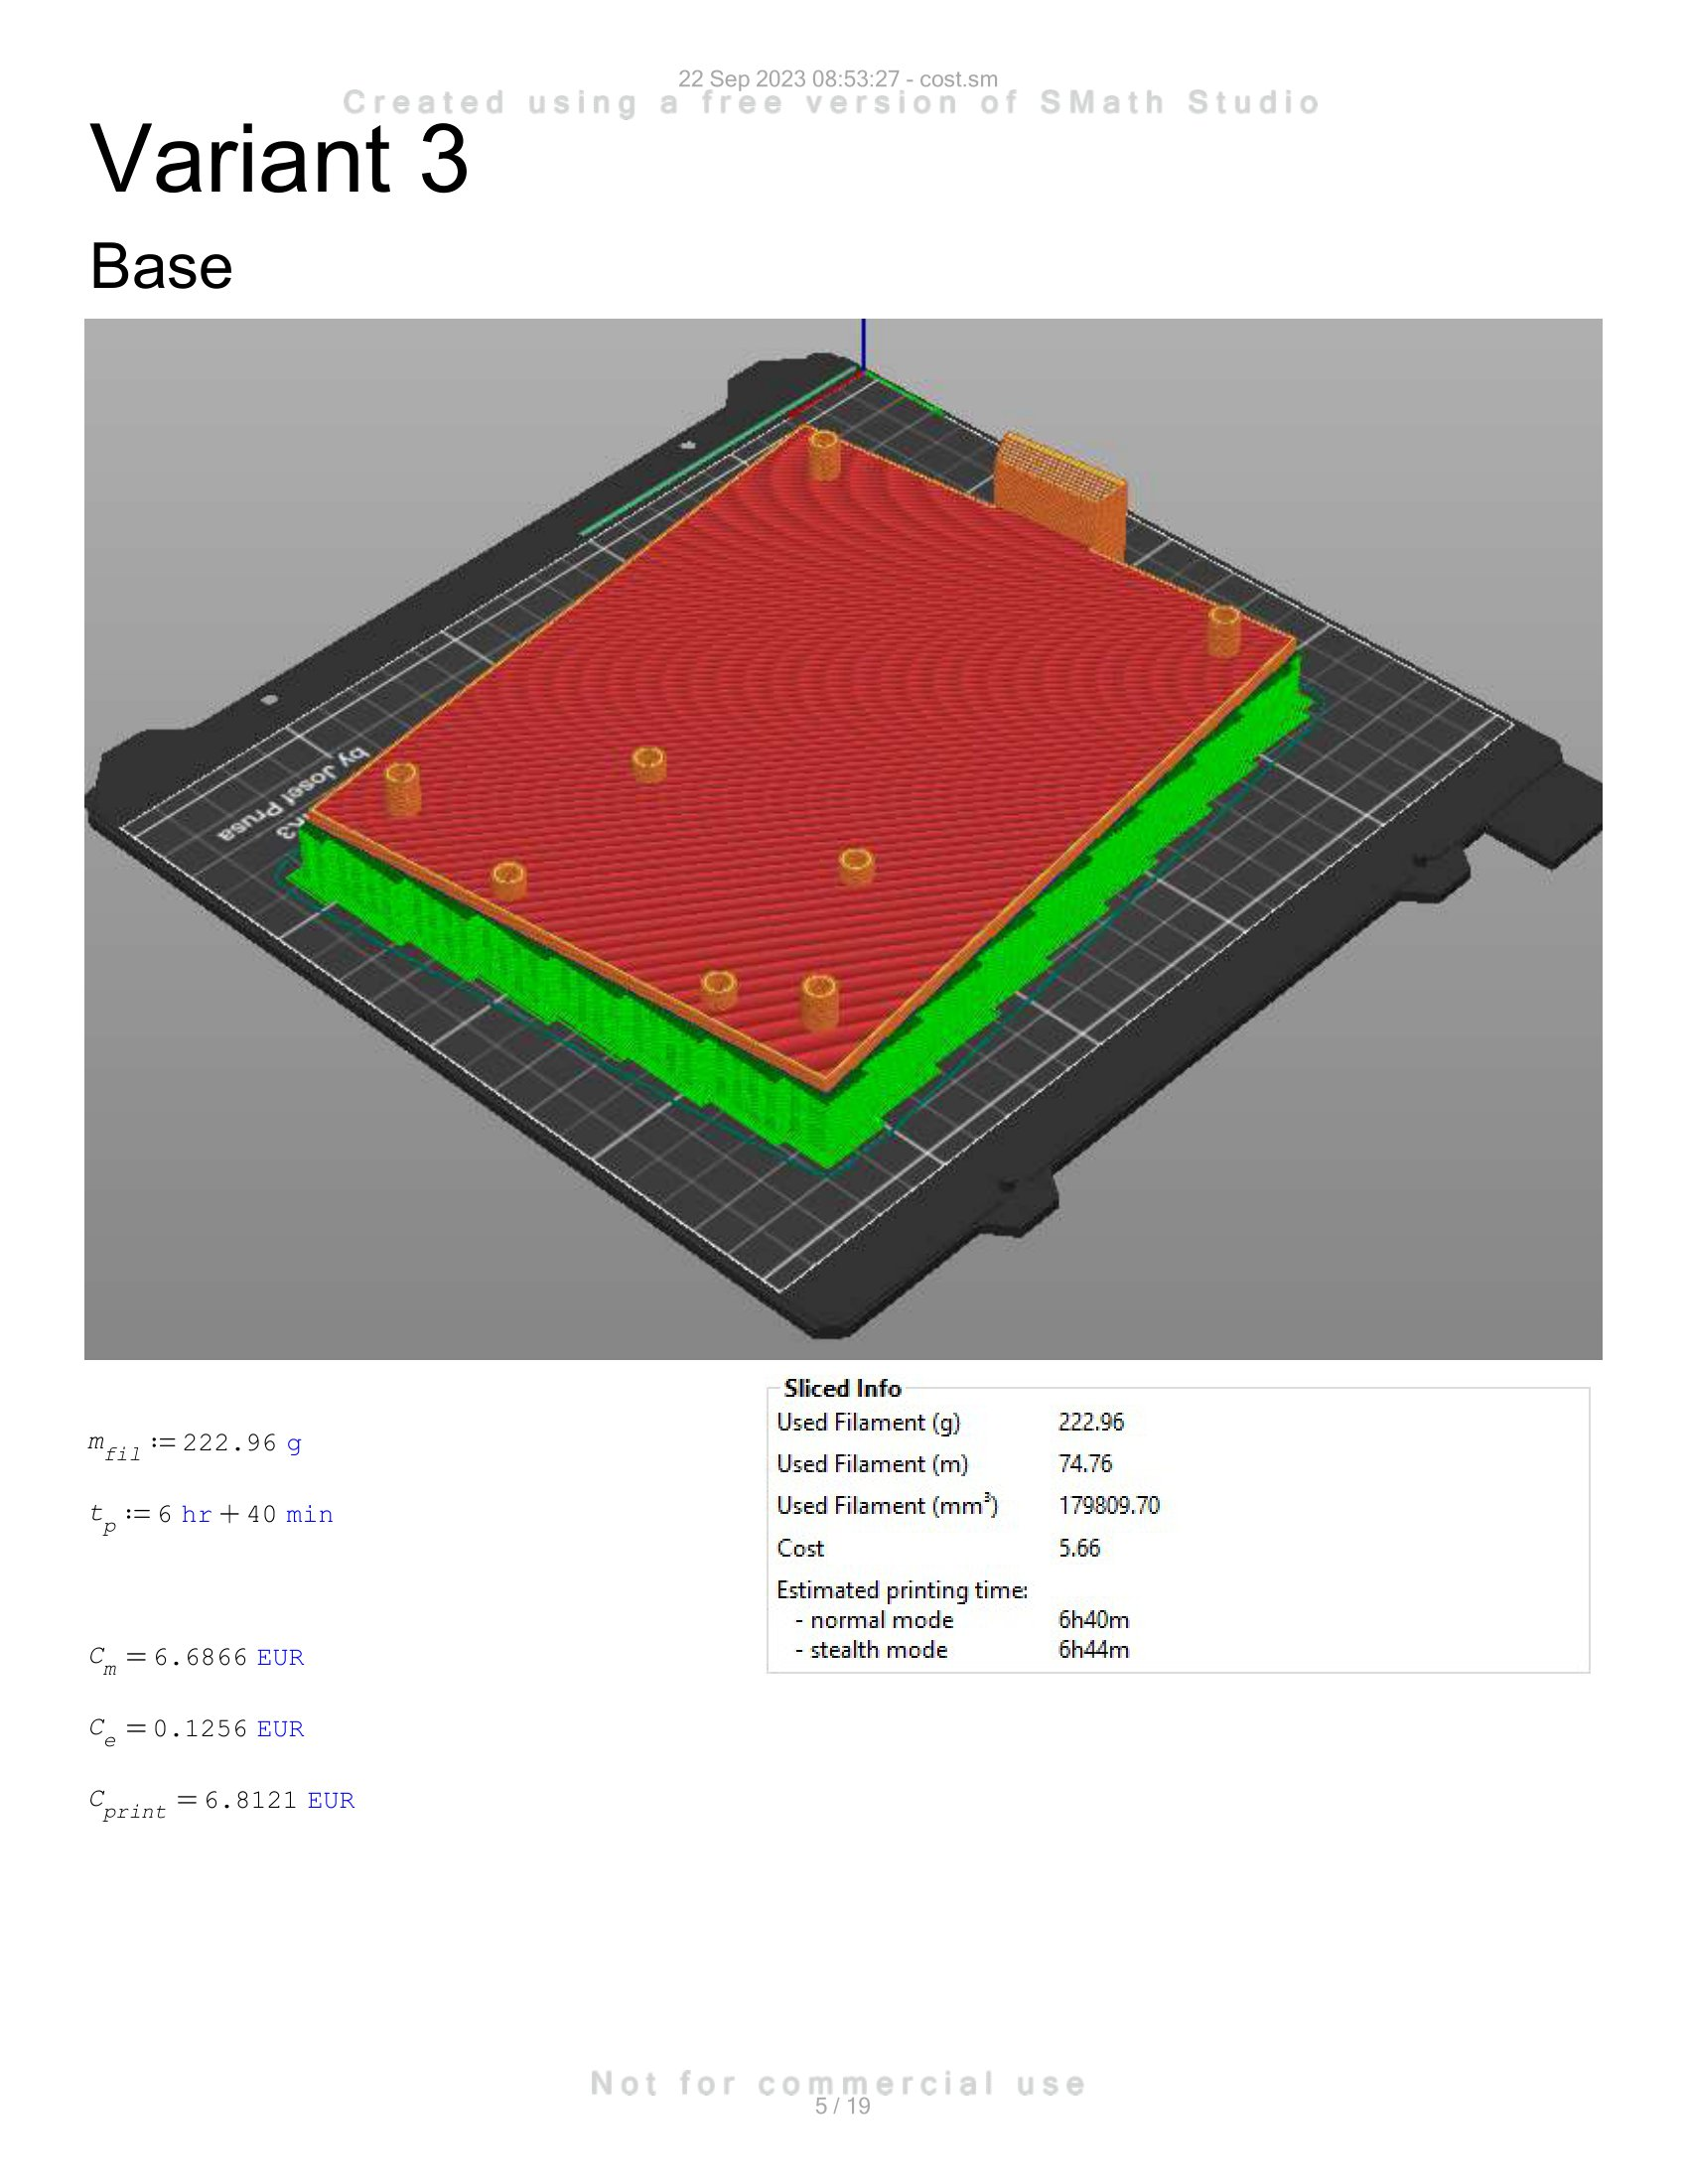
\includegraphics[width=\linewidth]{texs/appendix/data/costcalculation/cost1-05.jpg}
    \caption{Cost Calculation 5}
    \label{fig:cost-calculation-5}
\end{figure}

\begin{figure}[H]
    \centering
    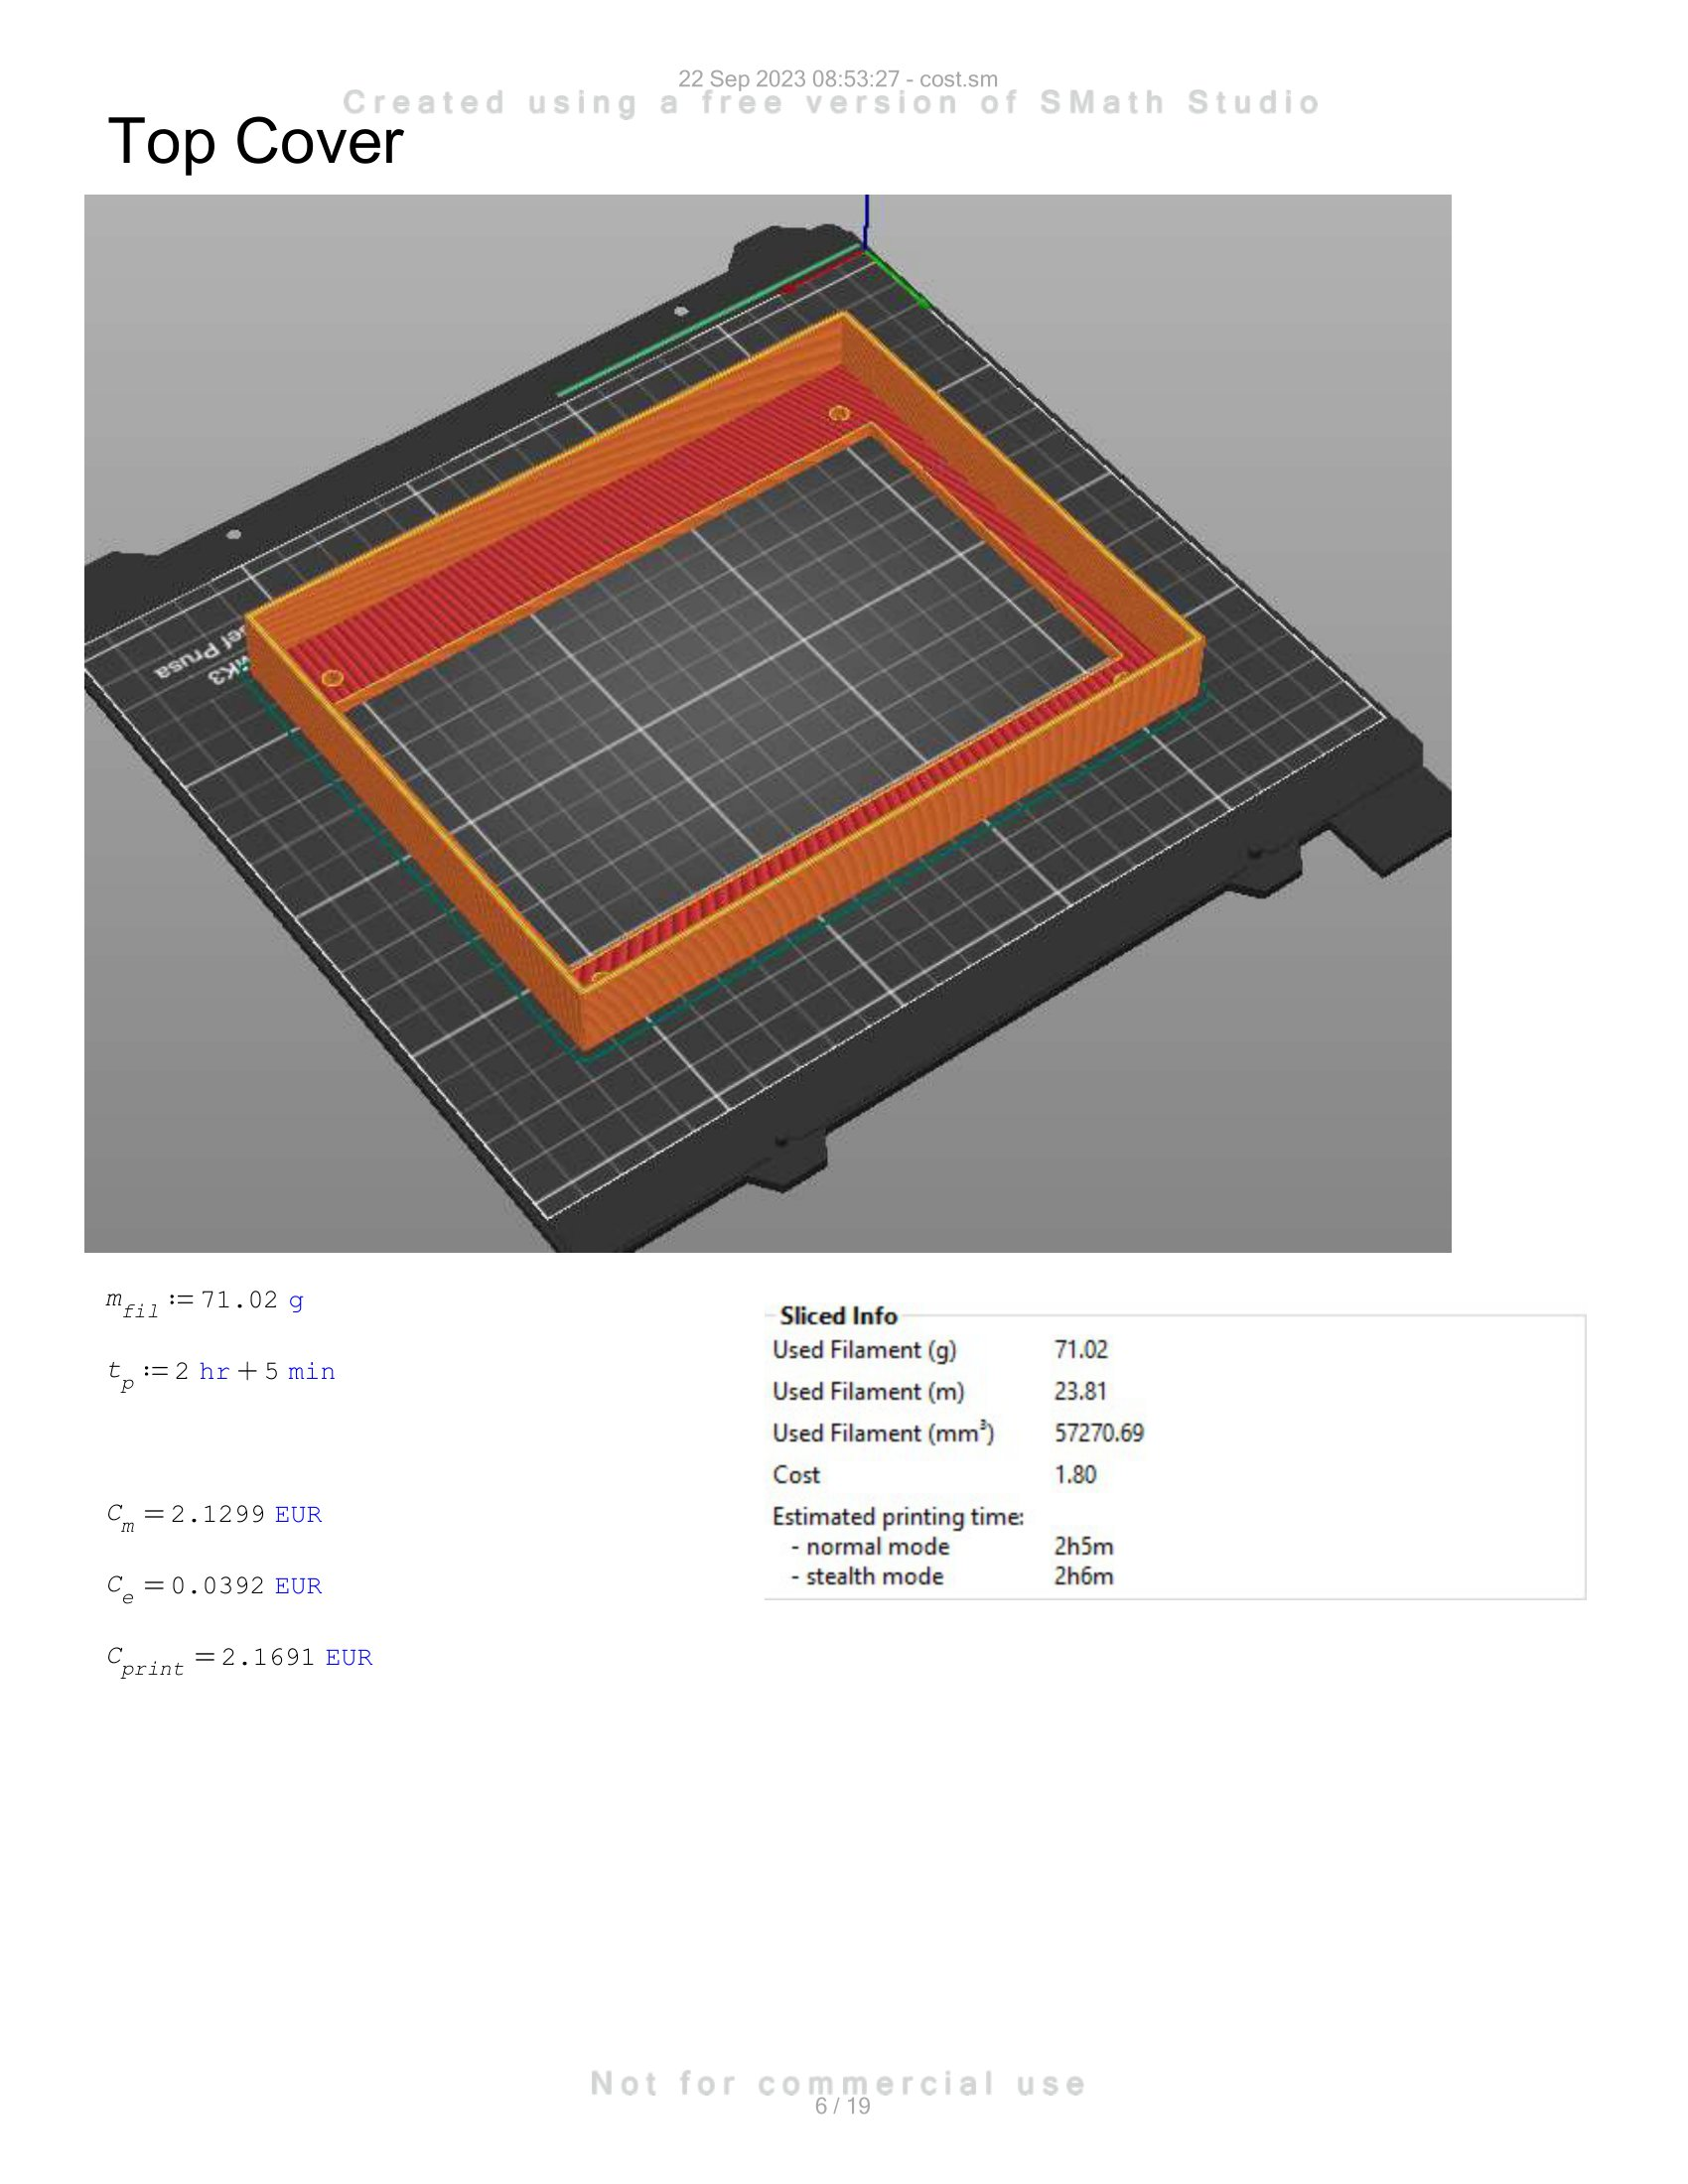
\includegraphics[width=\linewidth]{texs/appendix/data/costcalculation/cost1-06.jpg}
    \caption{Cost Calculation 6}
    \label{fig:cost-calculation-6}
\end{figure}

\begin{figure}[H]
    \centering
    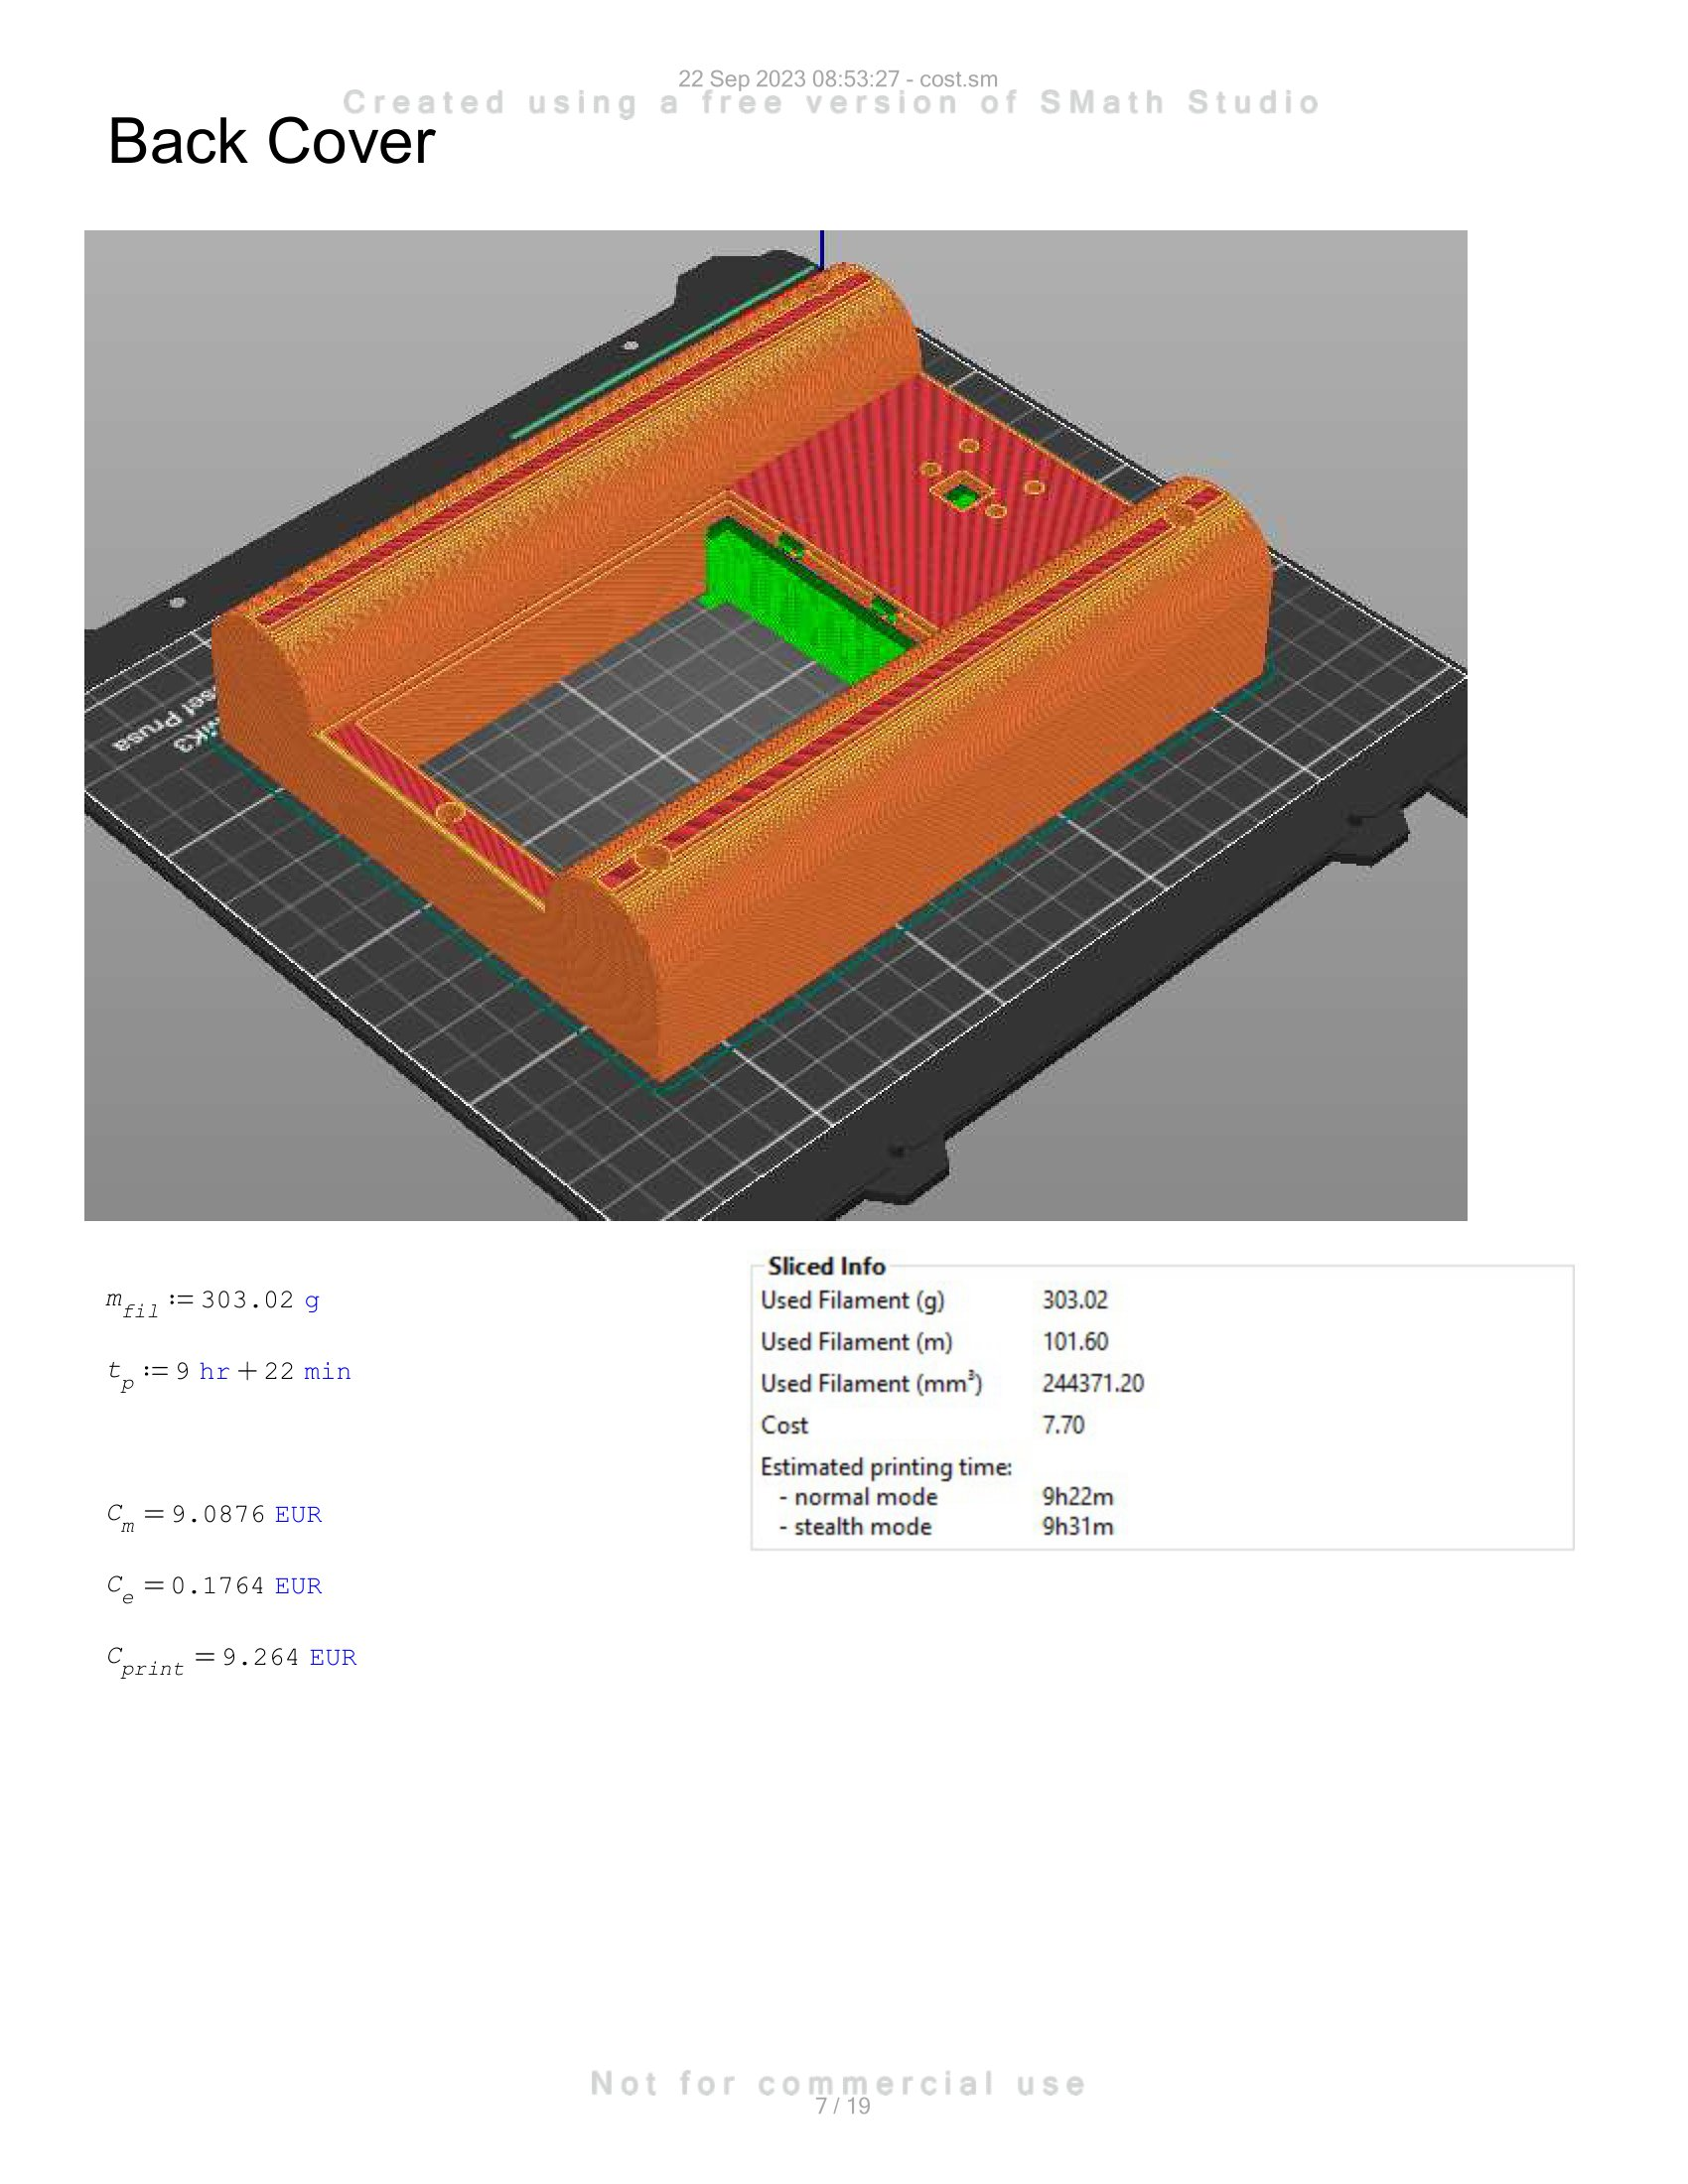
\includegraphics[width=\linewidth]{texs/appendix/data/costcalculation/cost1-07.jpg}
    \caption{Cost Calculation 7}
    \label{fig:cost-calculation-7}
\end{figure}

\begin{figure}[H]
    \centering
    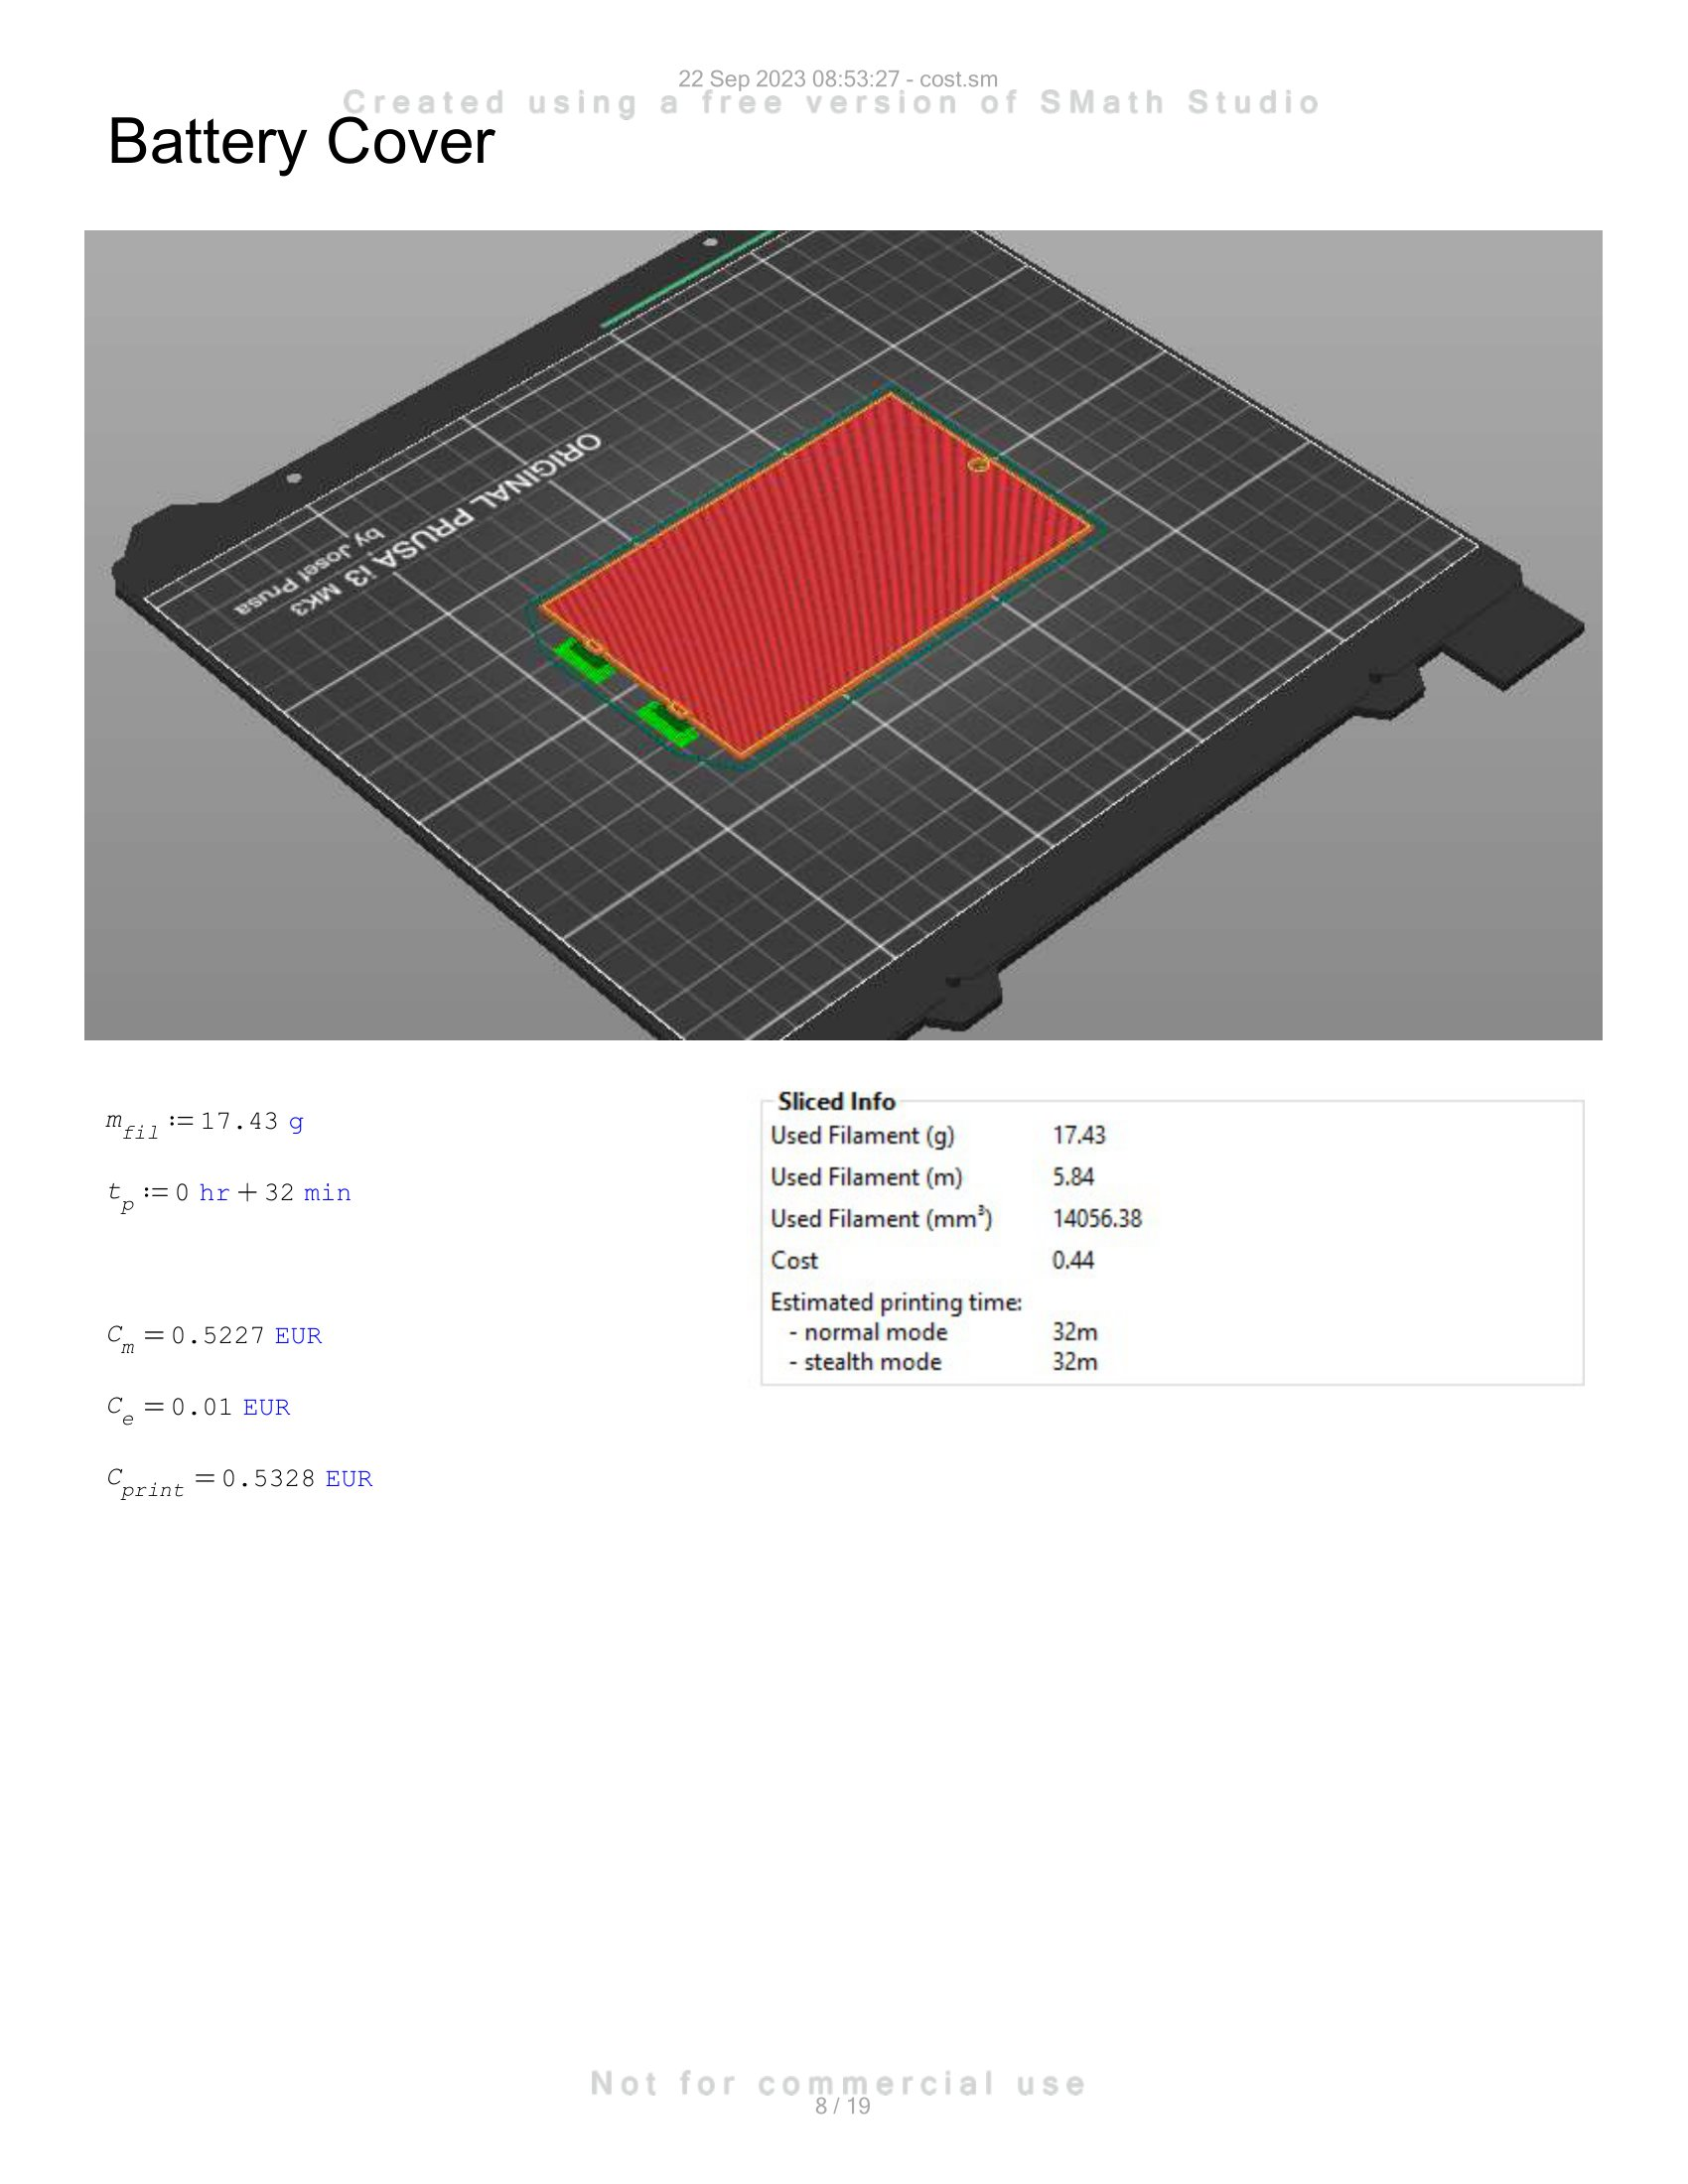
\includegraphics[width=\linewidth]{texs/appendix/data/costcalculation/cost1-08.jpg}
    \caption{Cost Calculation 8}
    \label{fig:cost-calculation-8}
\end{figure}

\begin{figure}[H]
    \centering
    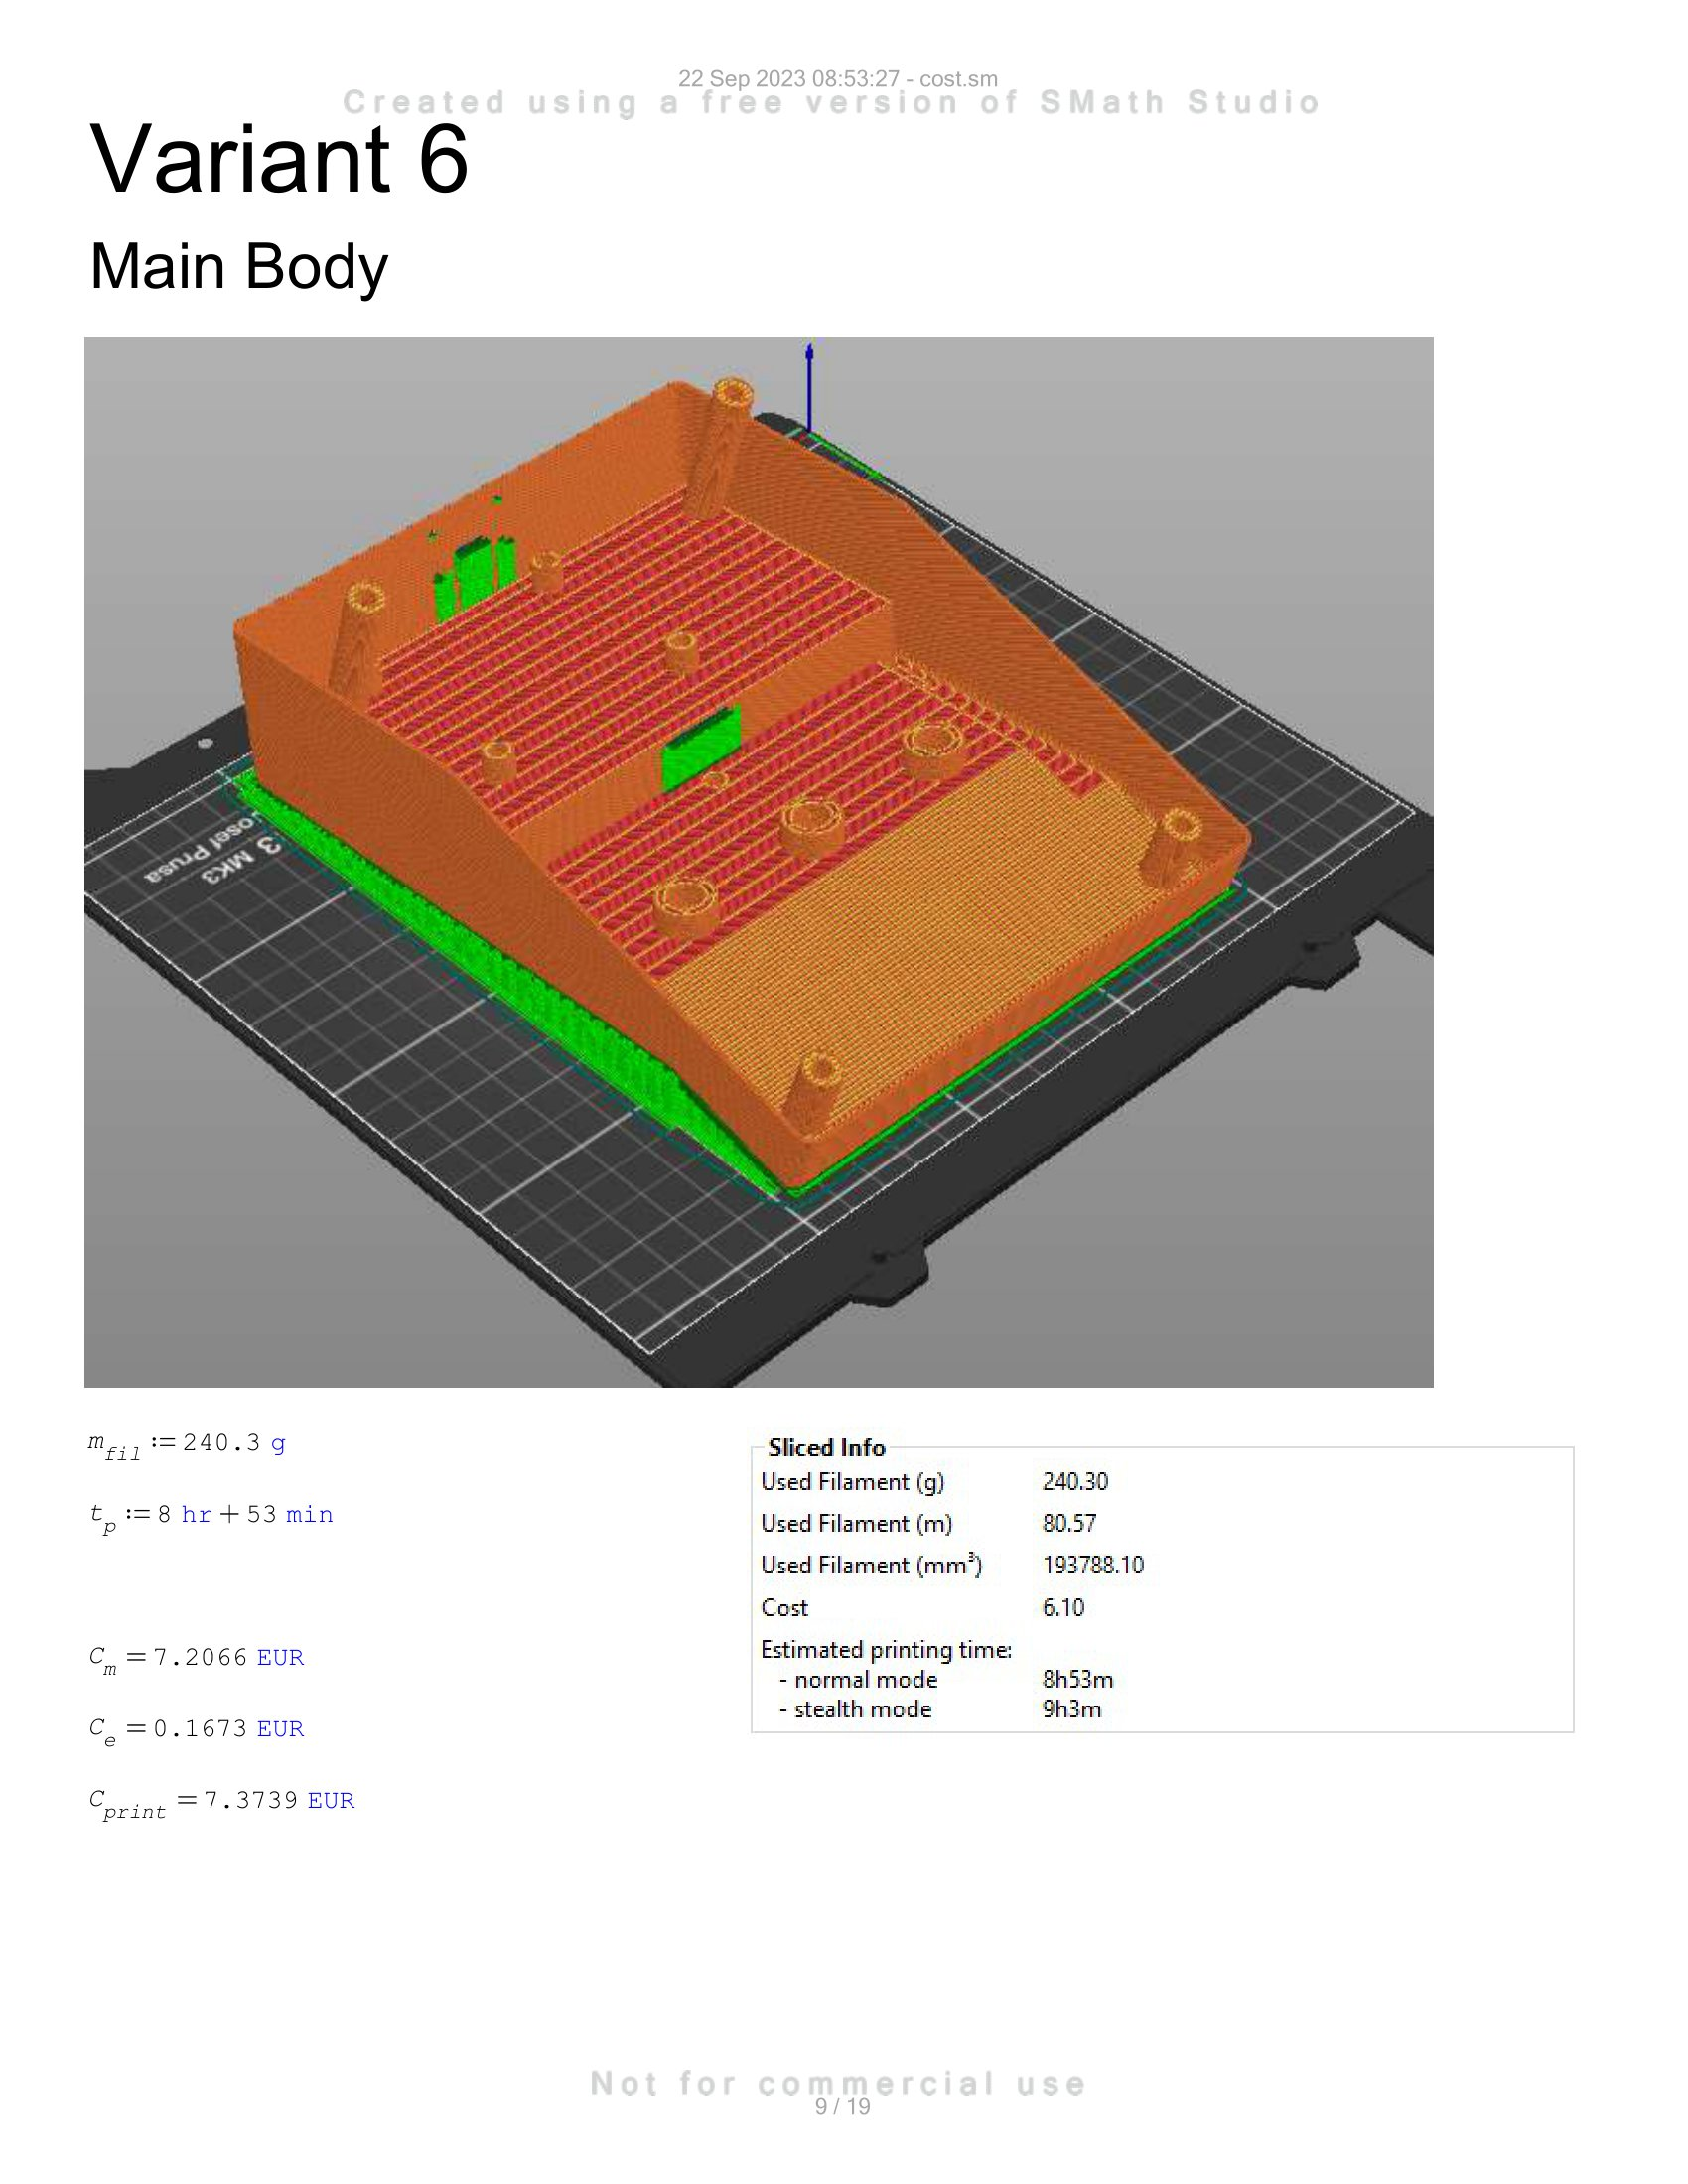
\includegraphics[width=\linewidth]{texs/appendix/data/costcalculation/cost1-09.jpg}
    \caption{Cost Calculation 9}
    \label{fig:cost-calculation-9}
\end{figure}

\begin{figure}[H]
    \centering
    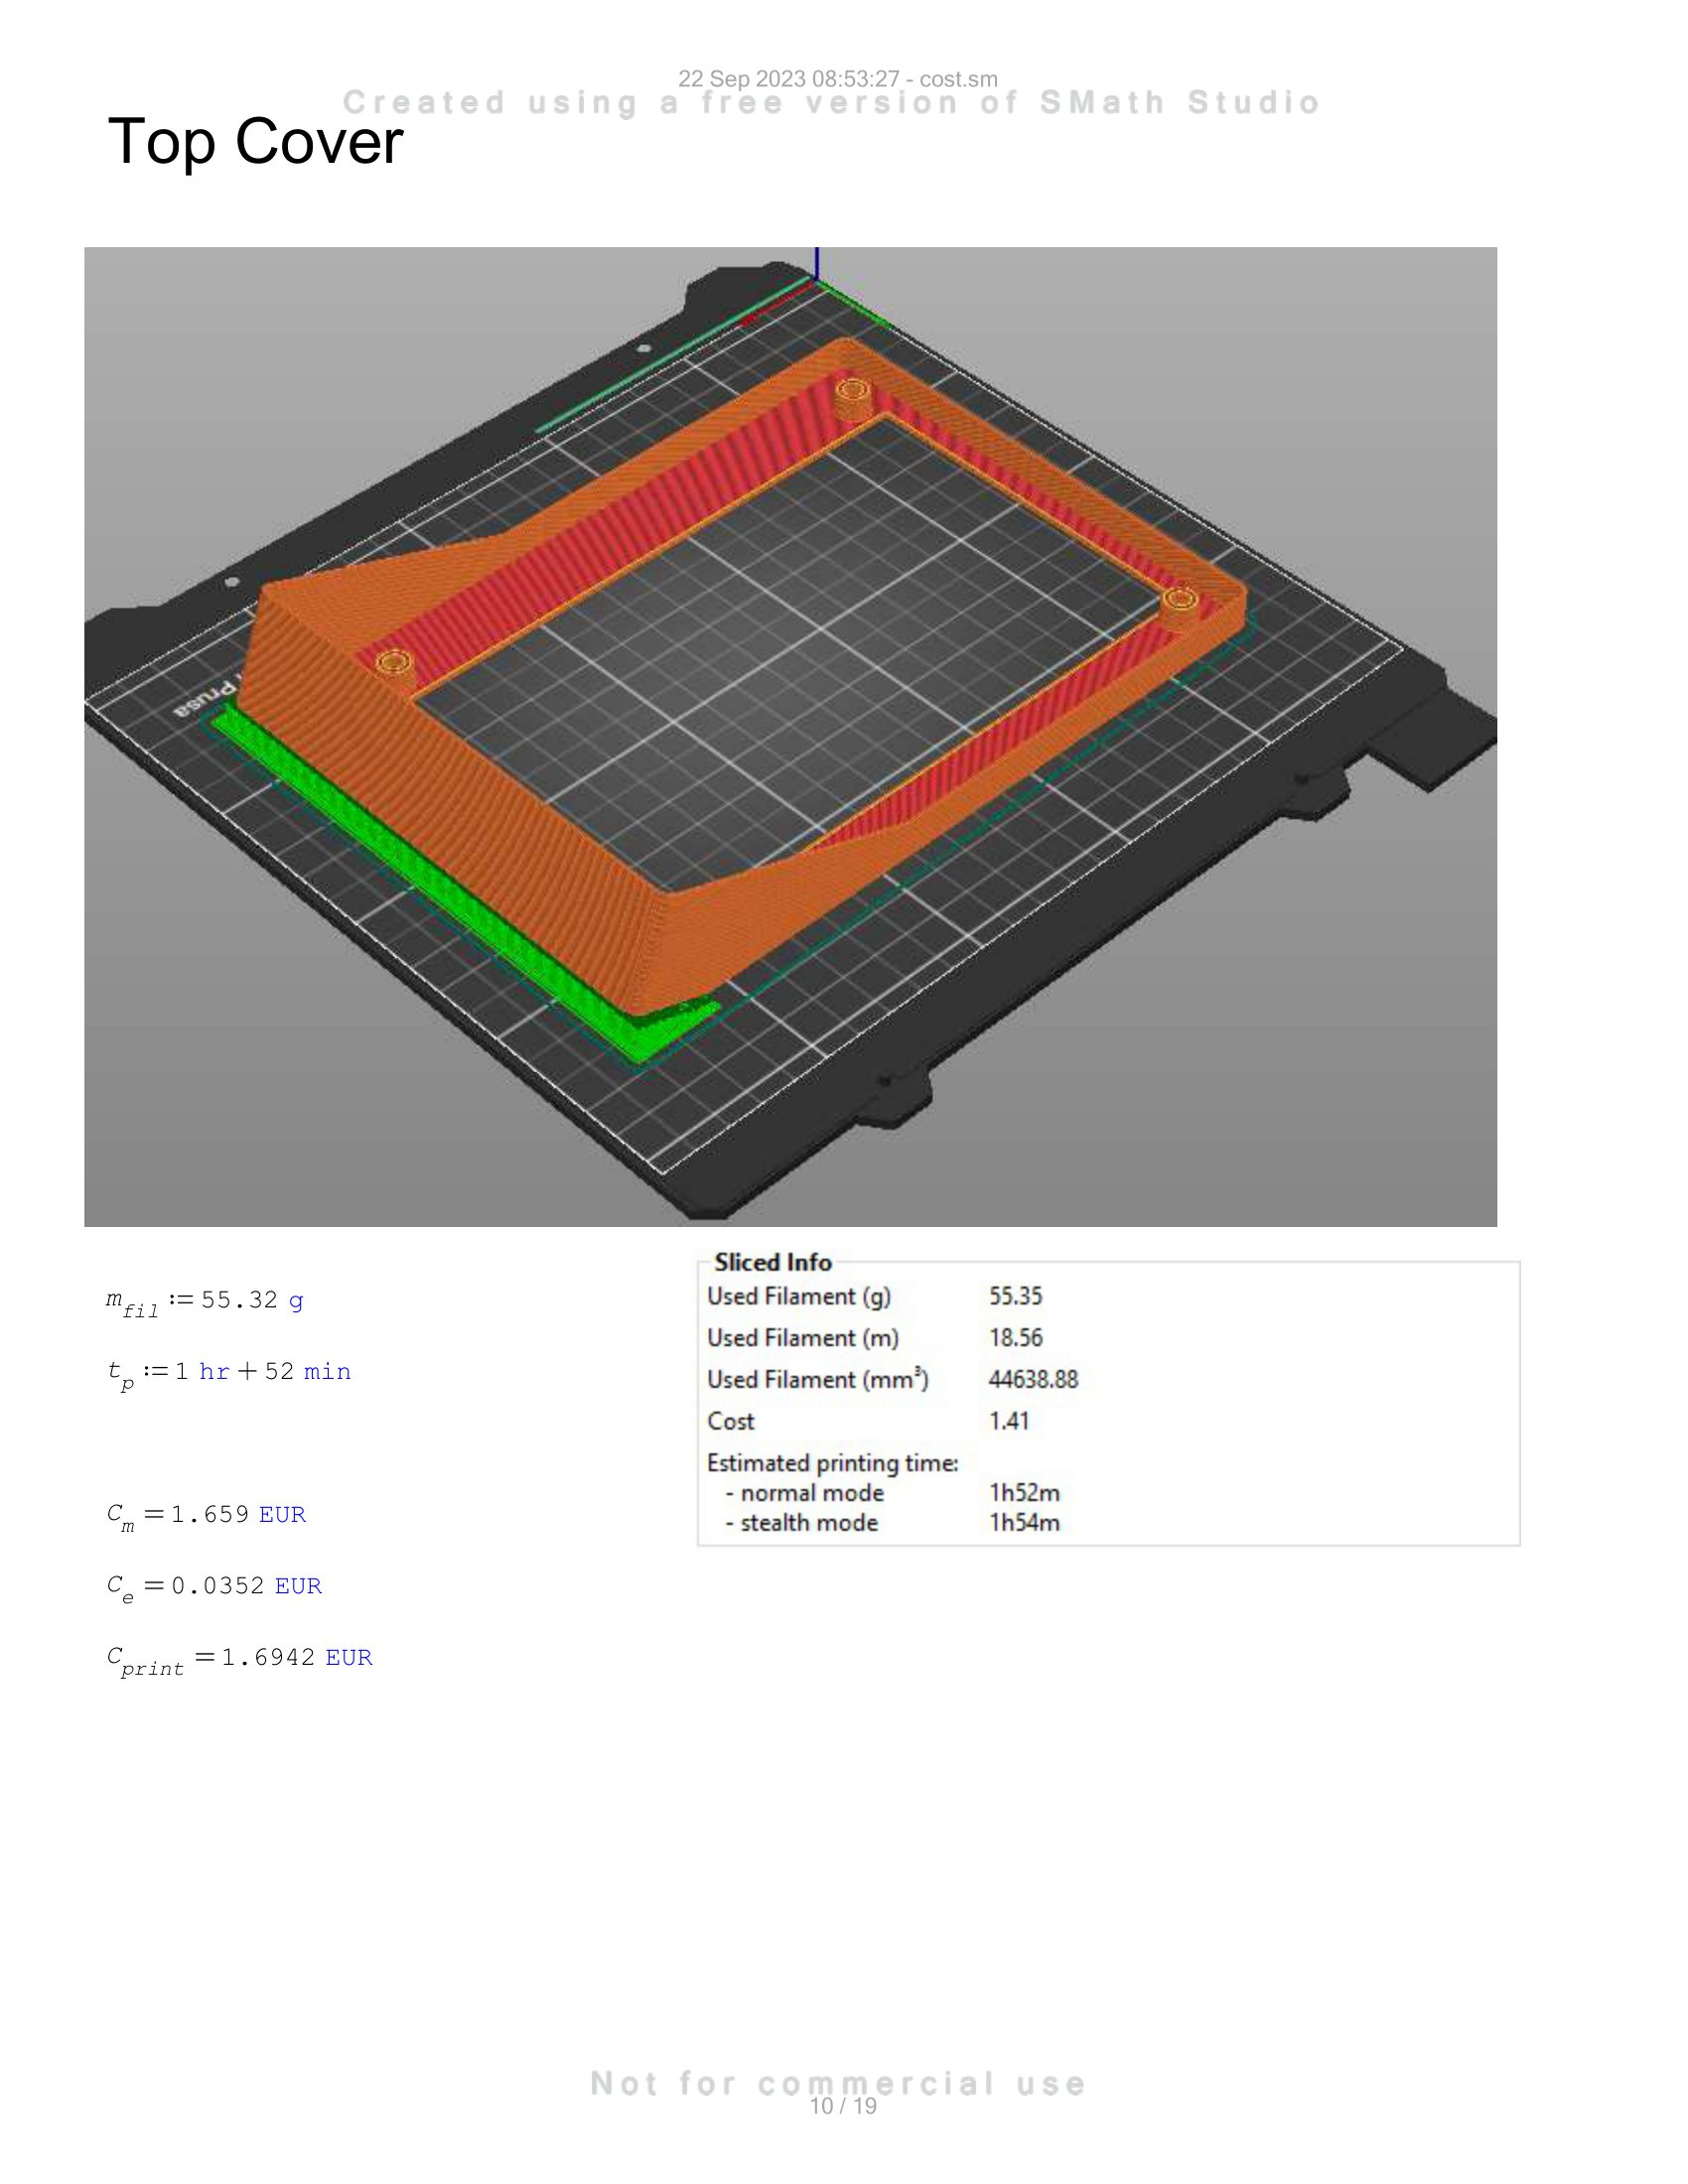
\includegraphics[width=\linewidth]{texs/appendix/data/costcalculation/cost1-10.jpg}
    \caption{Cost Calculation 10}
    \label{fig:cost-calculation-10}
\end{figure}

\begin{figure}[H]
    \centering
    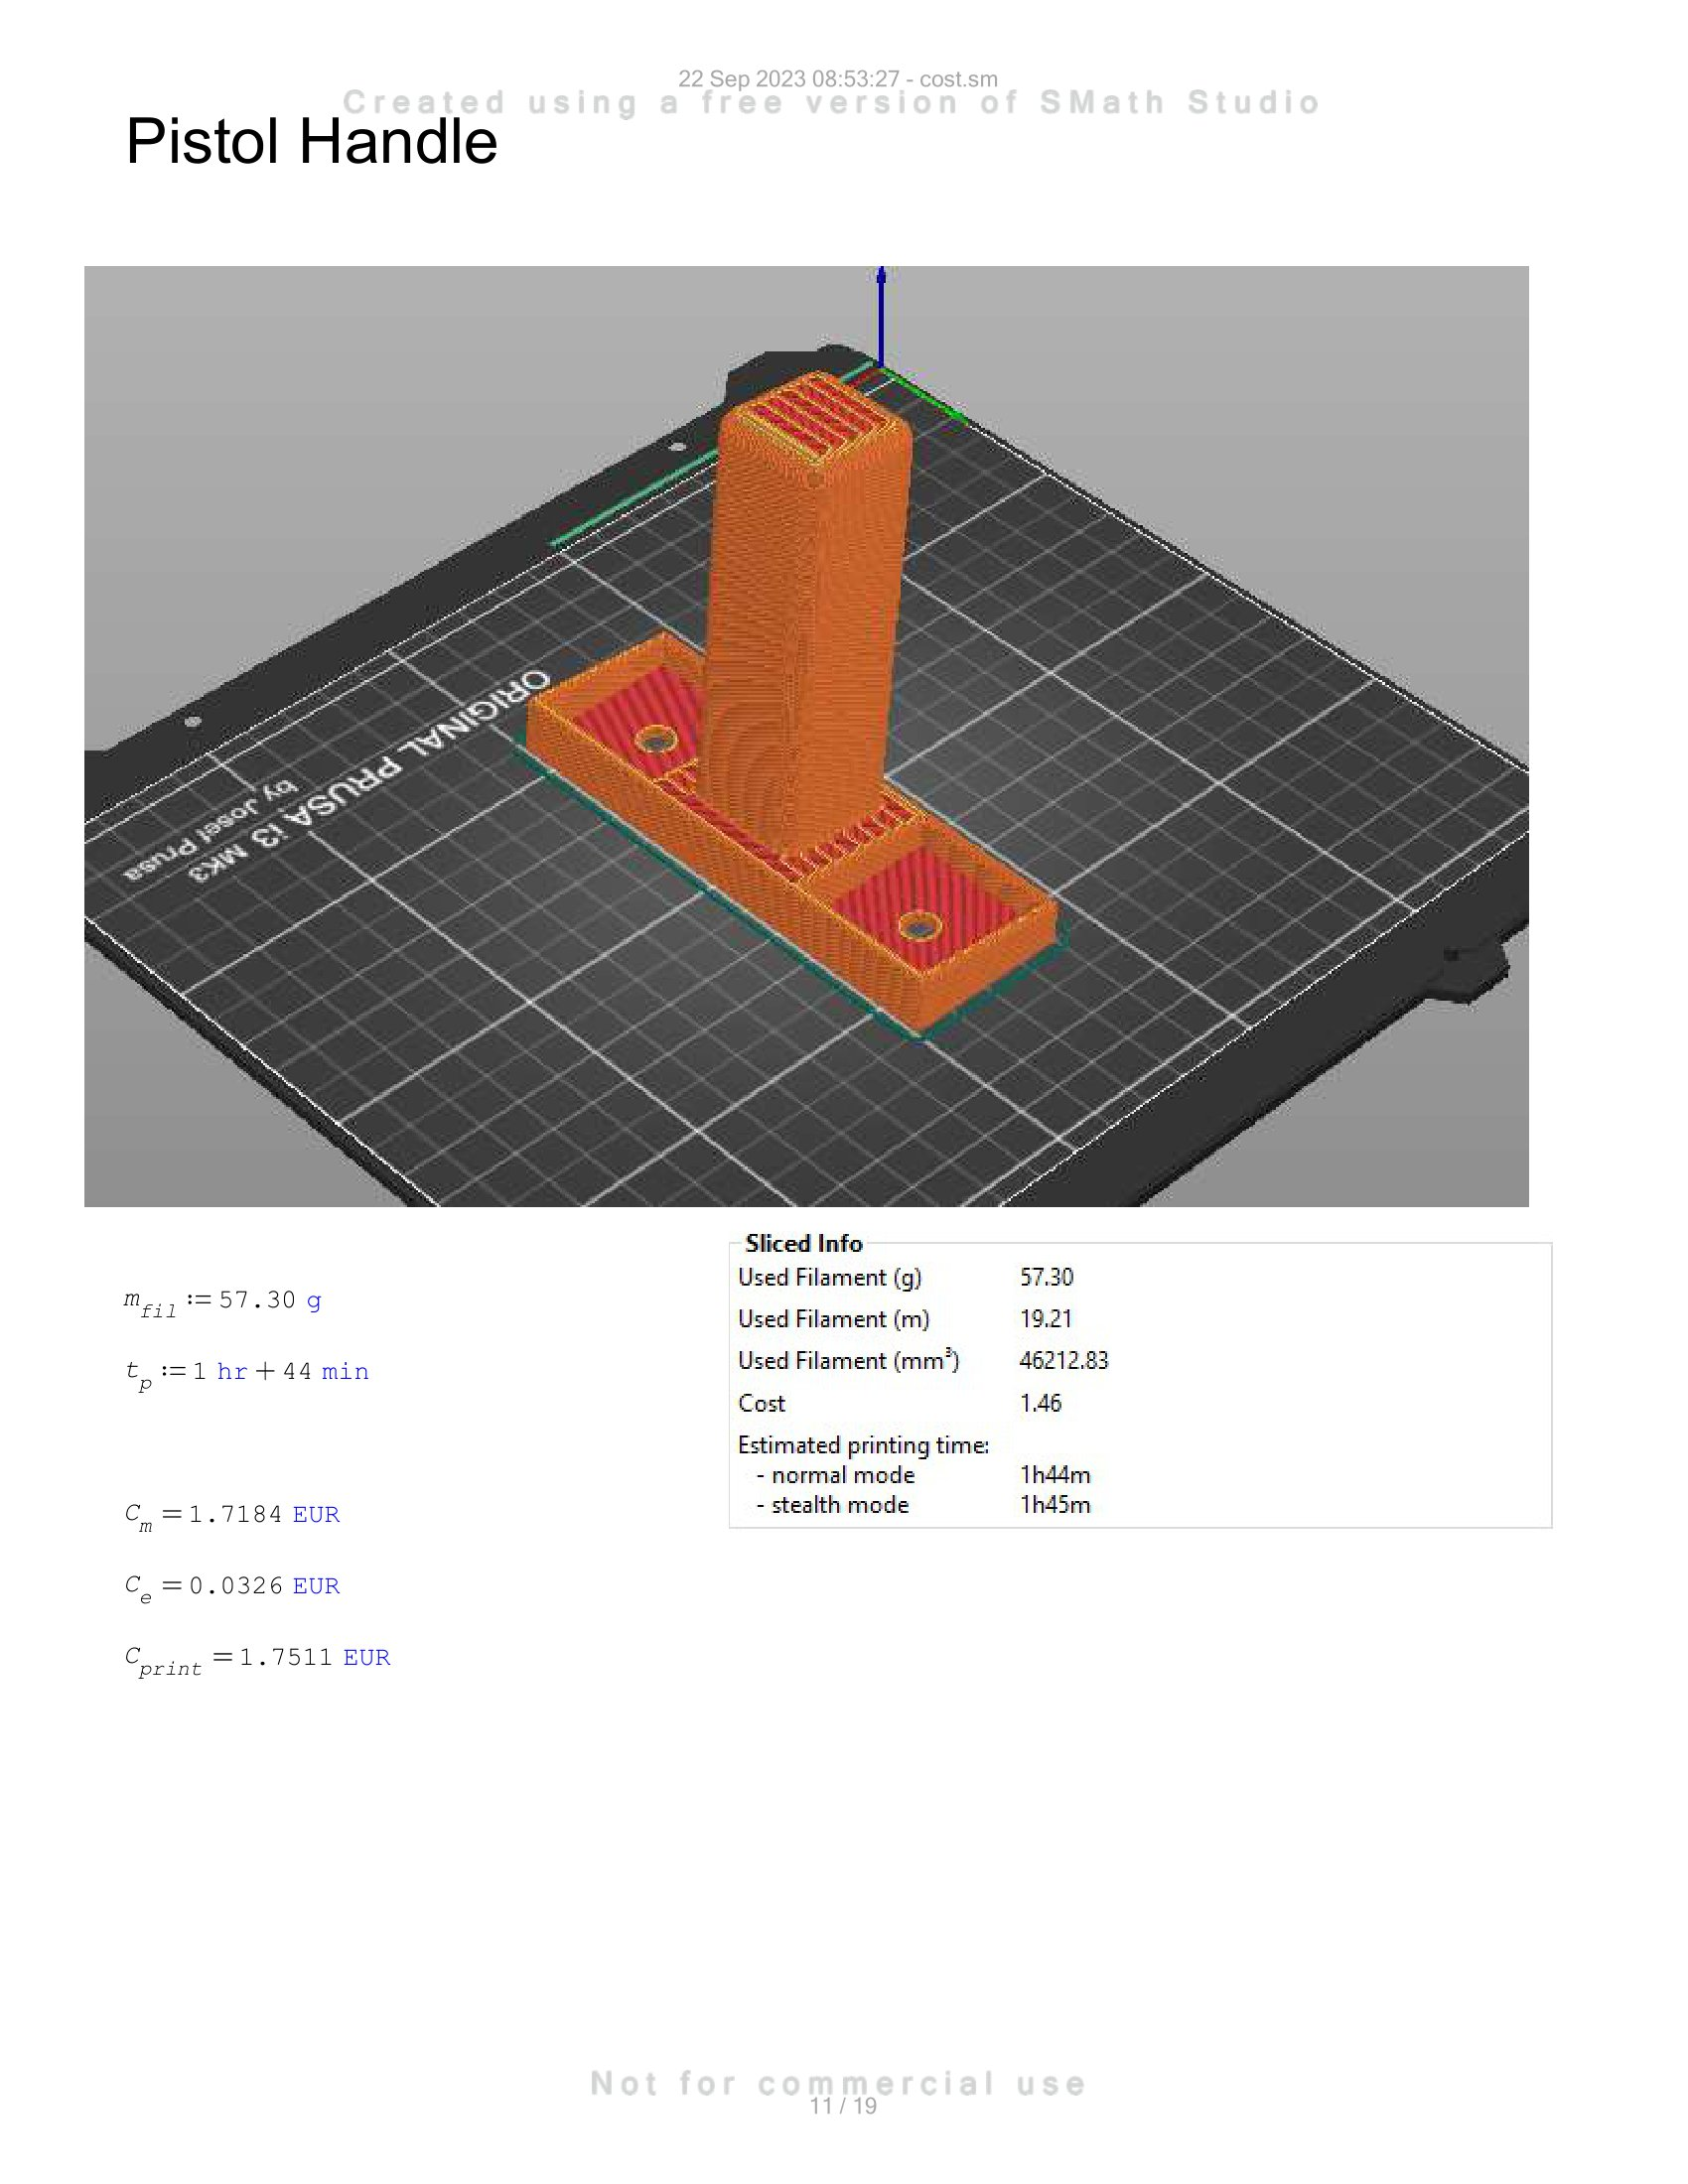
\includegraphics[width=\linewidth]{texs/appendix/data/costcalculation/cost1-11.jpg}
    \caption{Cost Calculation 11}
    \label{fig:cost-calculation-11}
\end{figure}

\begin{figure}[H]
    \centering
    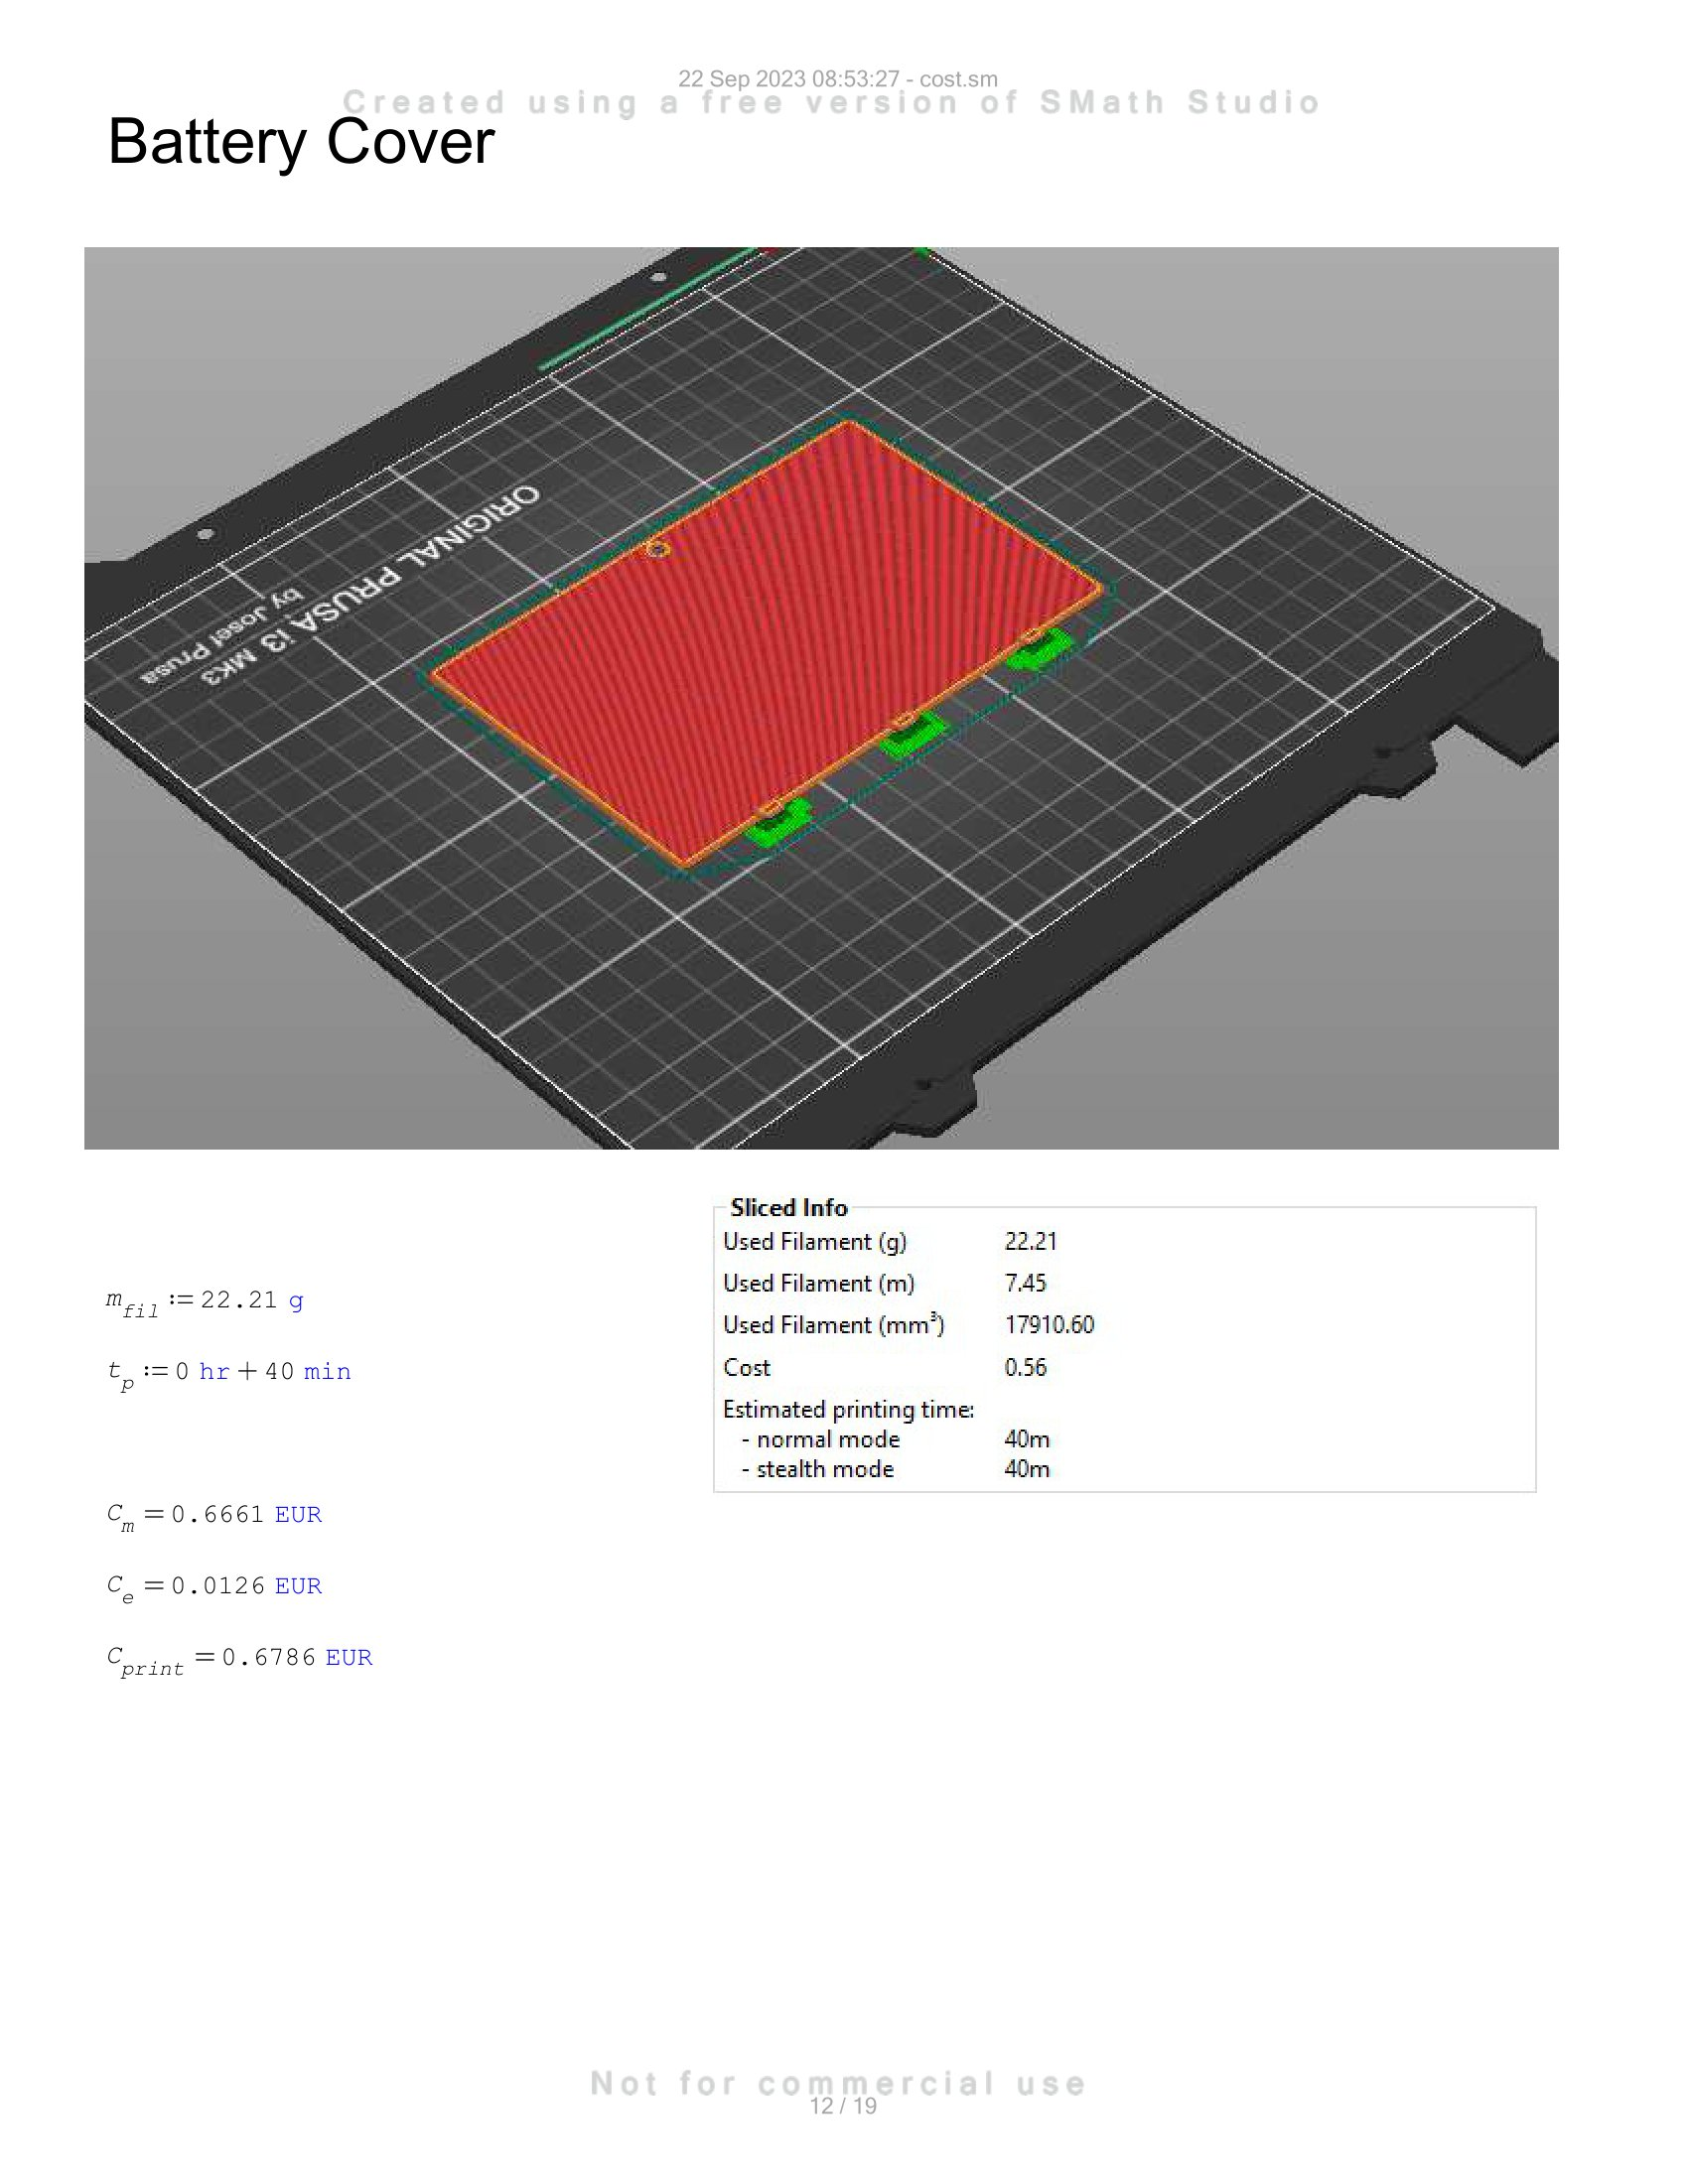
\includegraphics[width=\linewidth]{texs/appendix/data/costcalculation/cost1-12.jpg}
    \caption{Cost Calculation 12}
    \label{fig:cost-calculation-12}
\end{figure}

\begin{figure}[H]
    \centering
    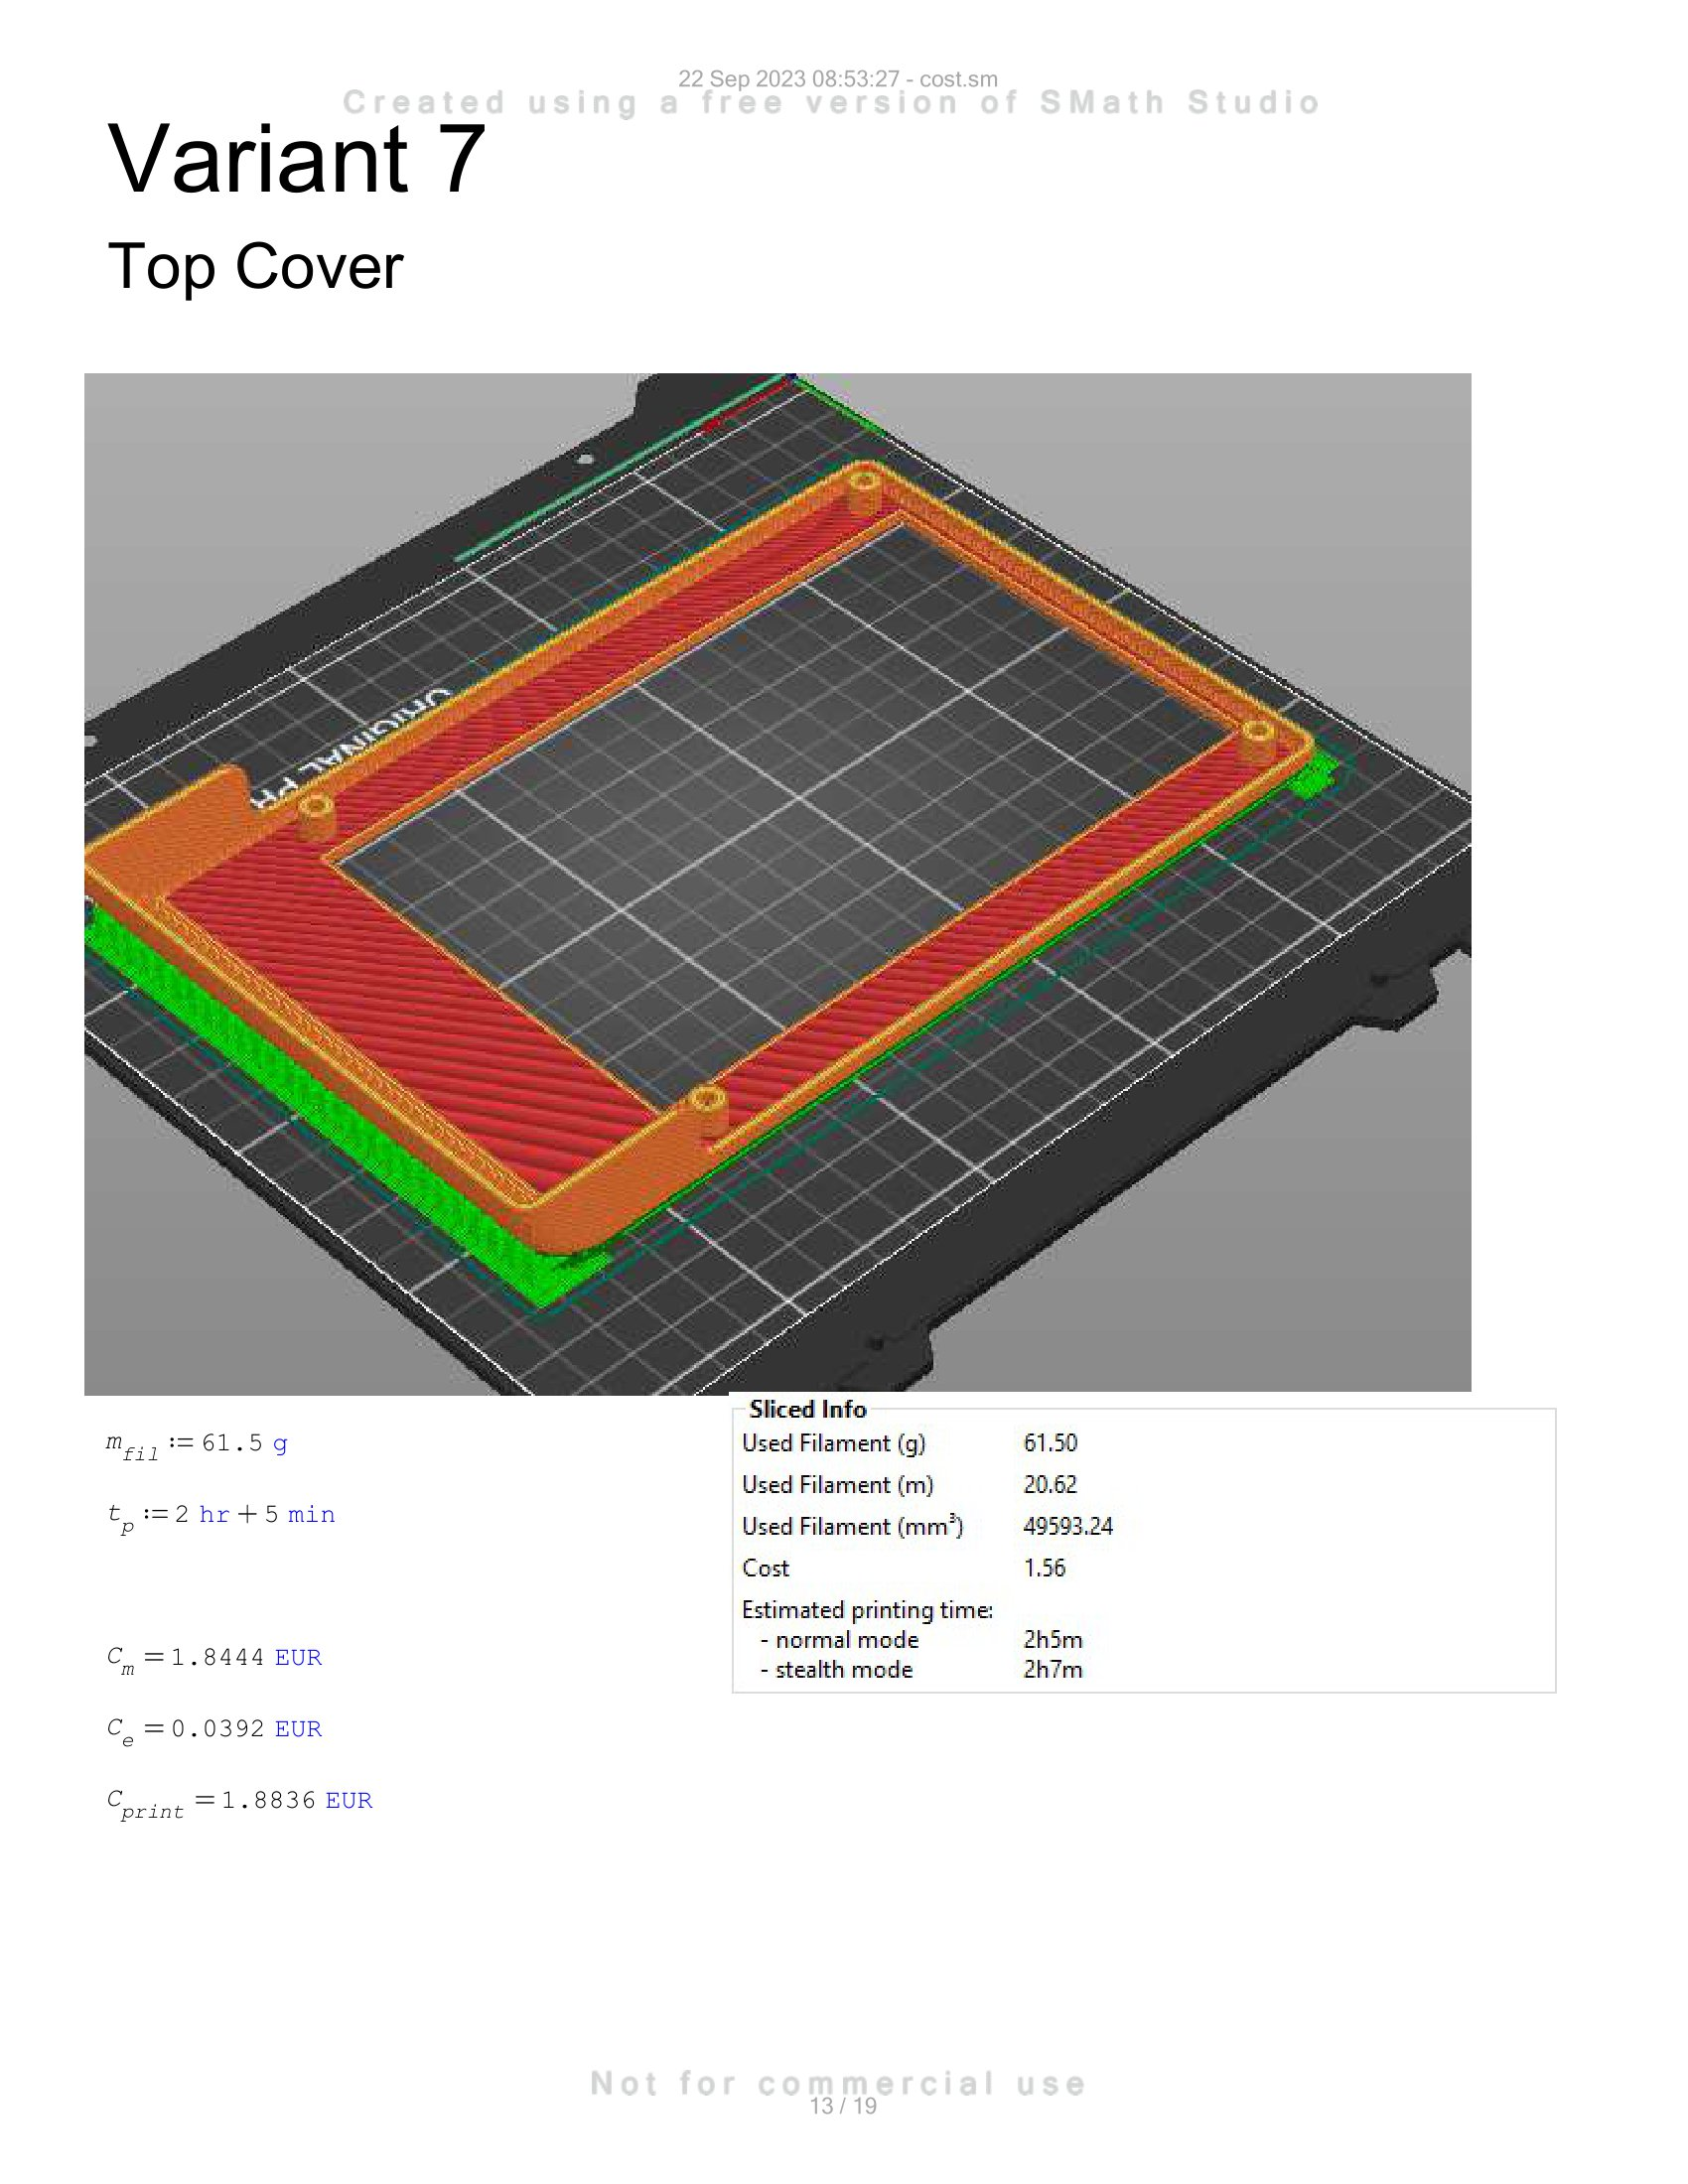
\includegraphics[width=\linewidth]{texs/appendix/data/costcalculation/cost1-13.jpg}
    \caption{Cost Calculation 13}
    \label{fig:cost-calculation-13}
\end{figure}

\begin{figure}[H]
    \centering
    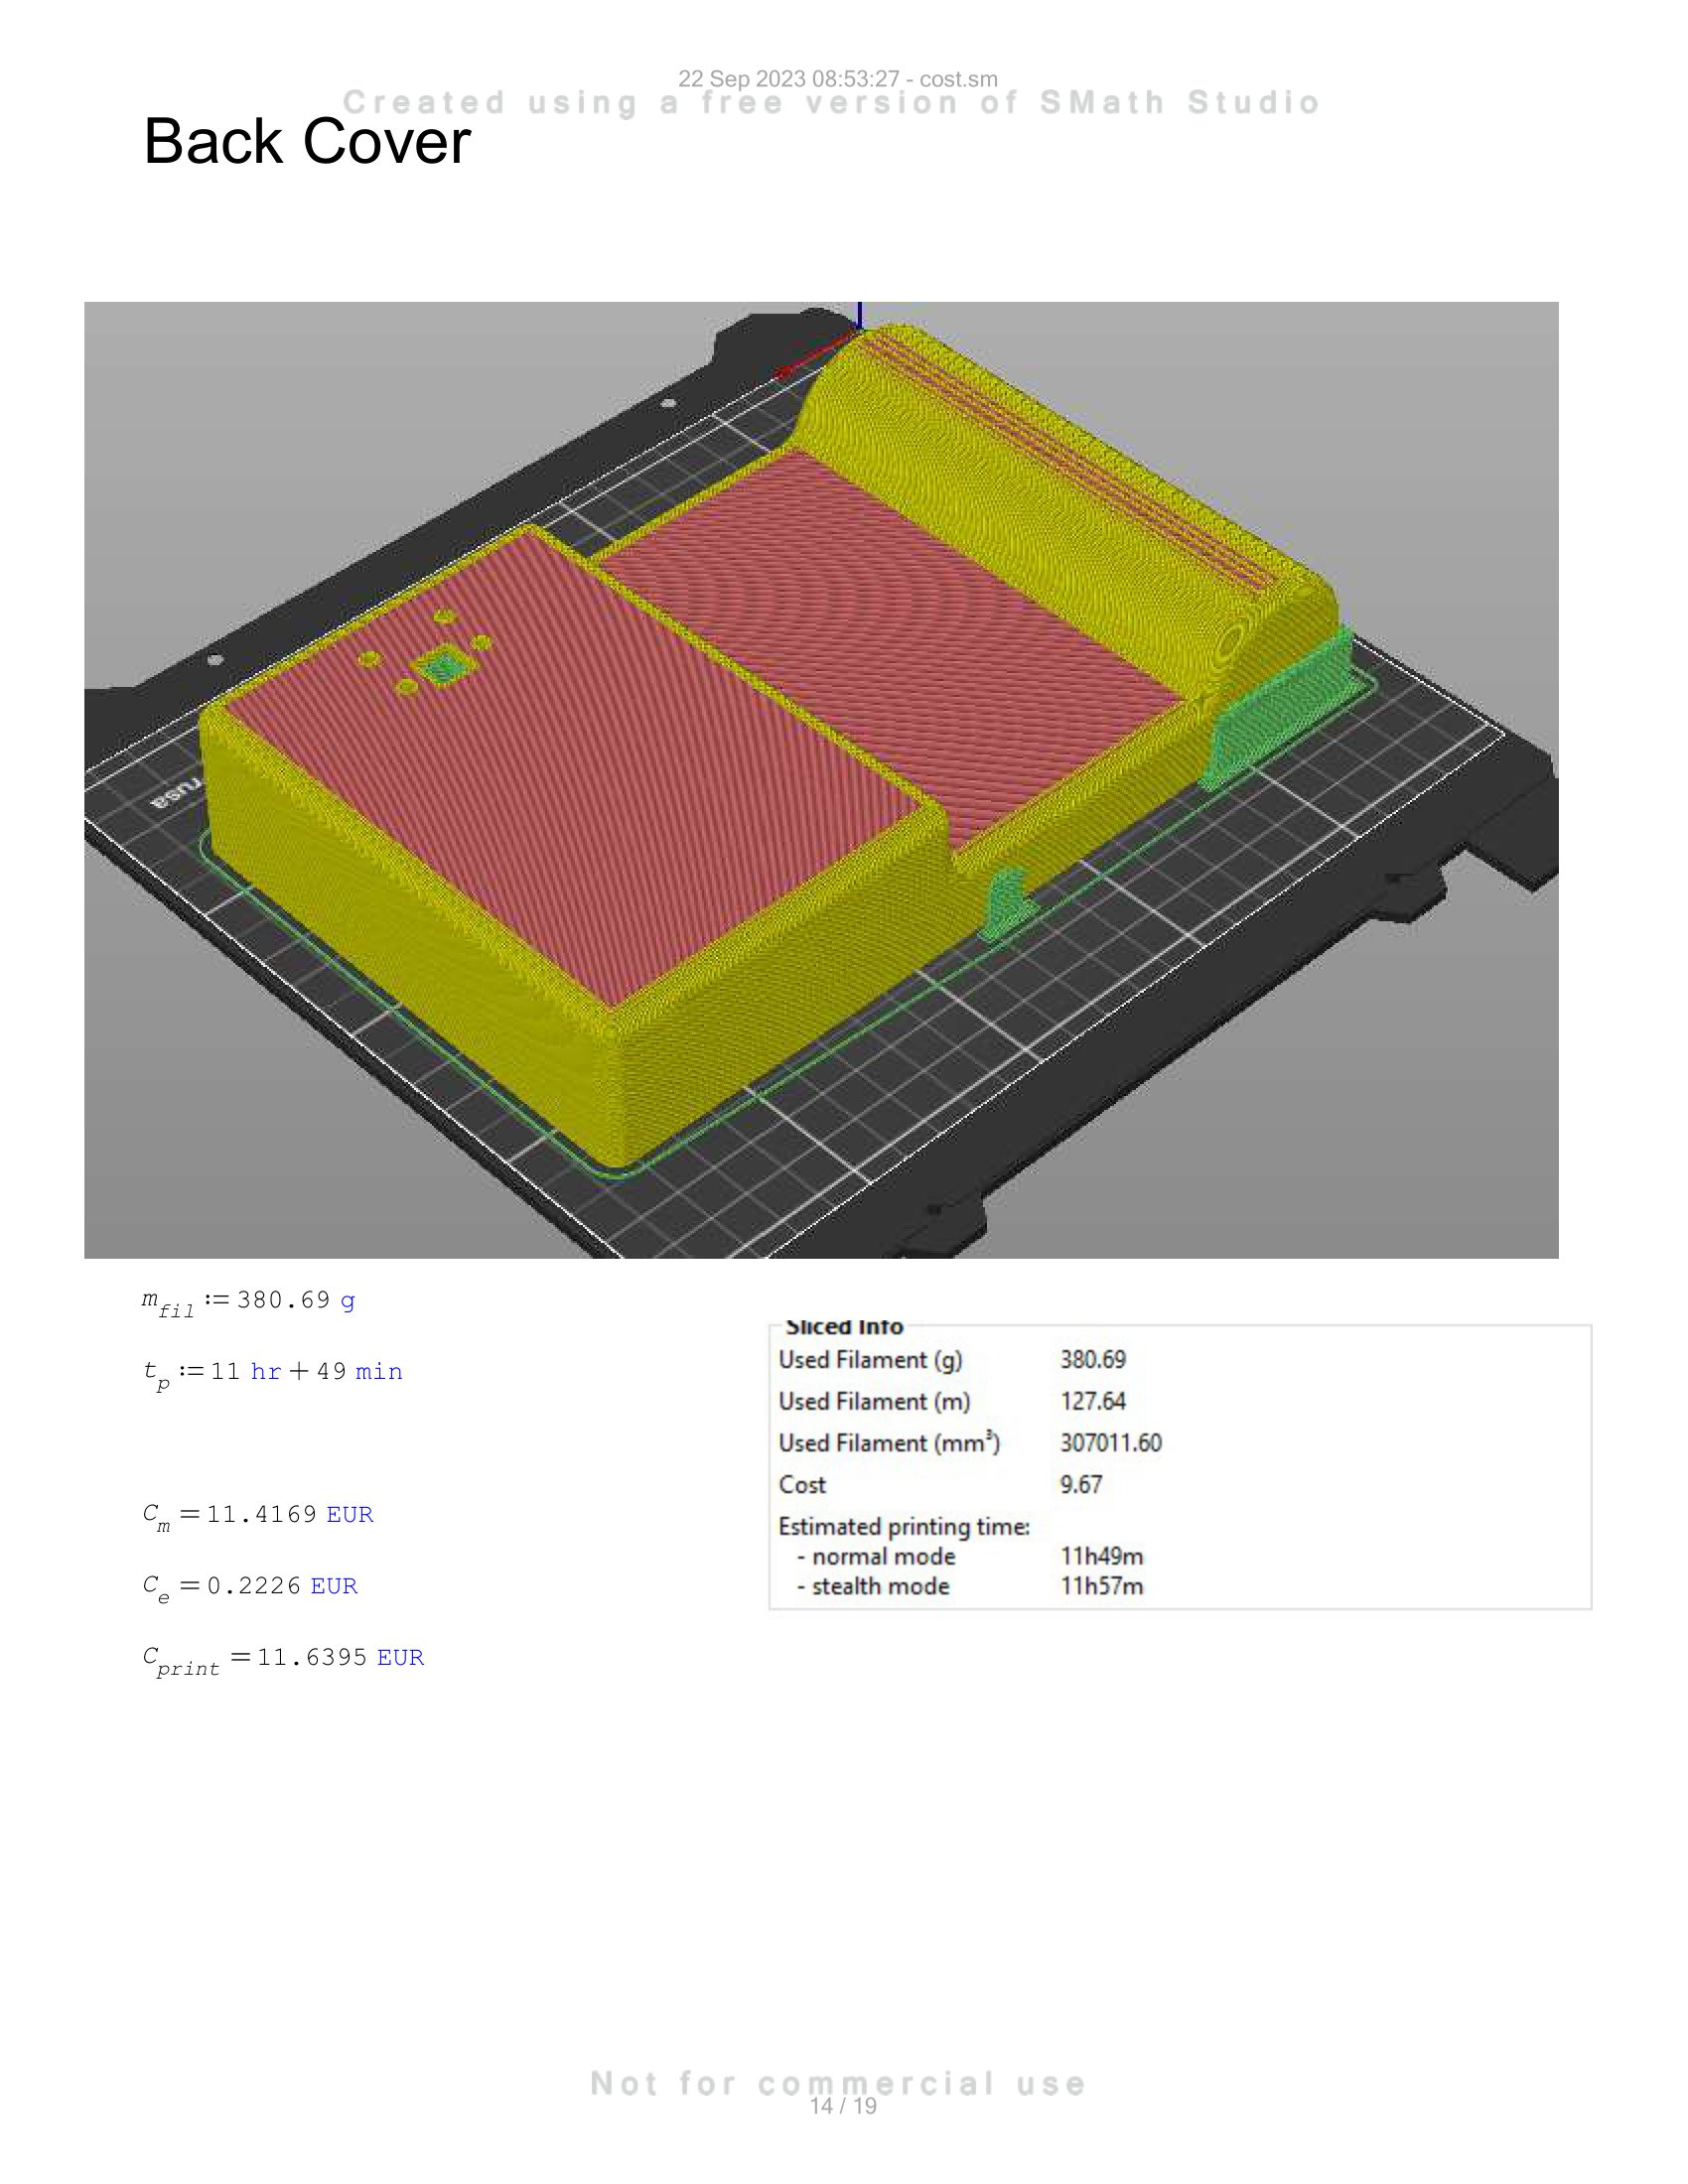
\includegraphics[width=\linewidth]{texs/appendix/data/costcalculation/cost1-14.jpg}
    \caption{Cost Calculation 14}
    \label{fig:cost-calculation-14}
\end{figure}

\begin{figure}[H]
    \centering
    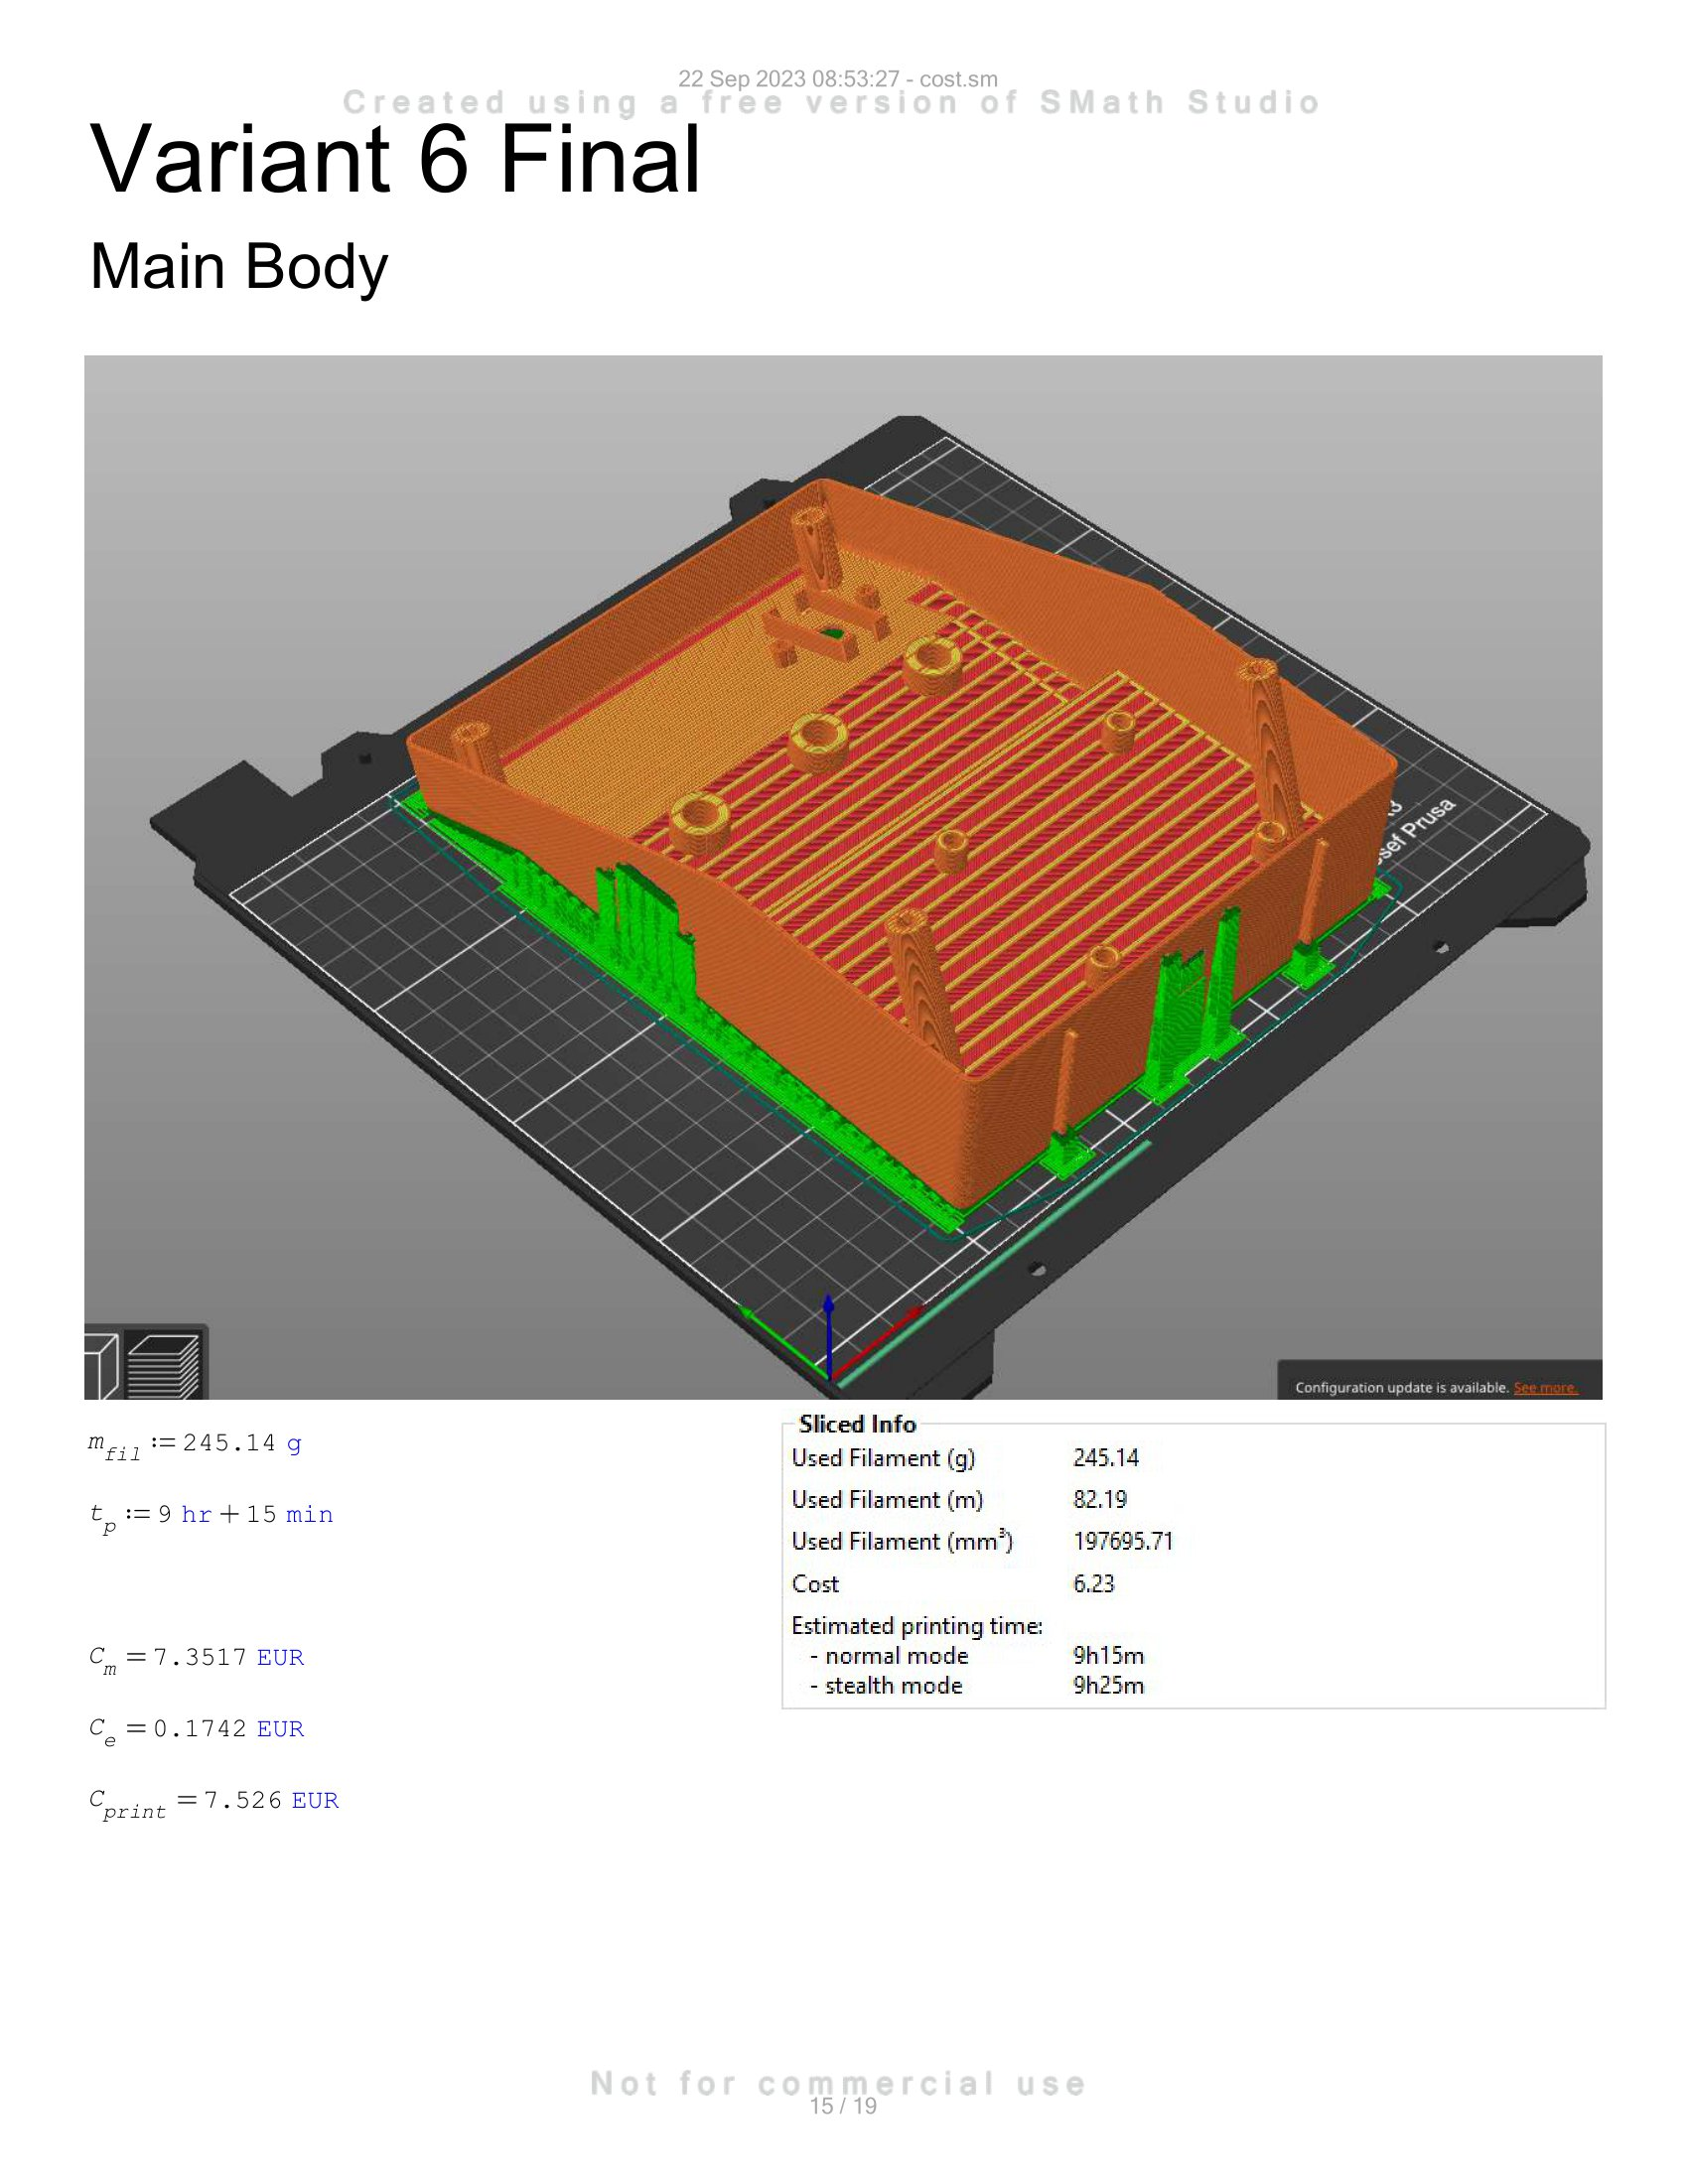
\includegraphics[width=\linewidth]{texs/appendix/data/costcalculation/cost1-15.jpg}
    \caption{Cost Calculation 15}
    \label{fig:cost-calculation-15}
\end{figure}

\begin{figure}[H]
    \centering
    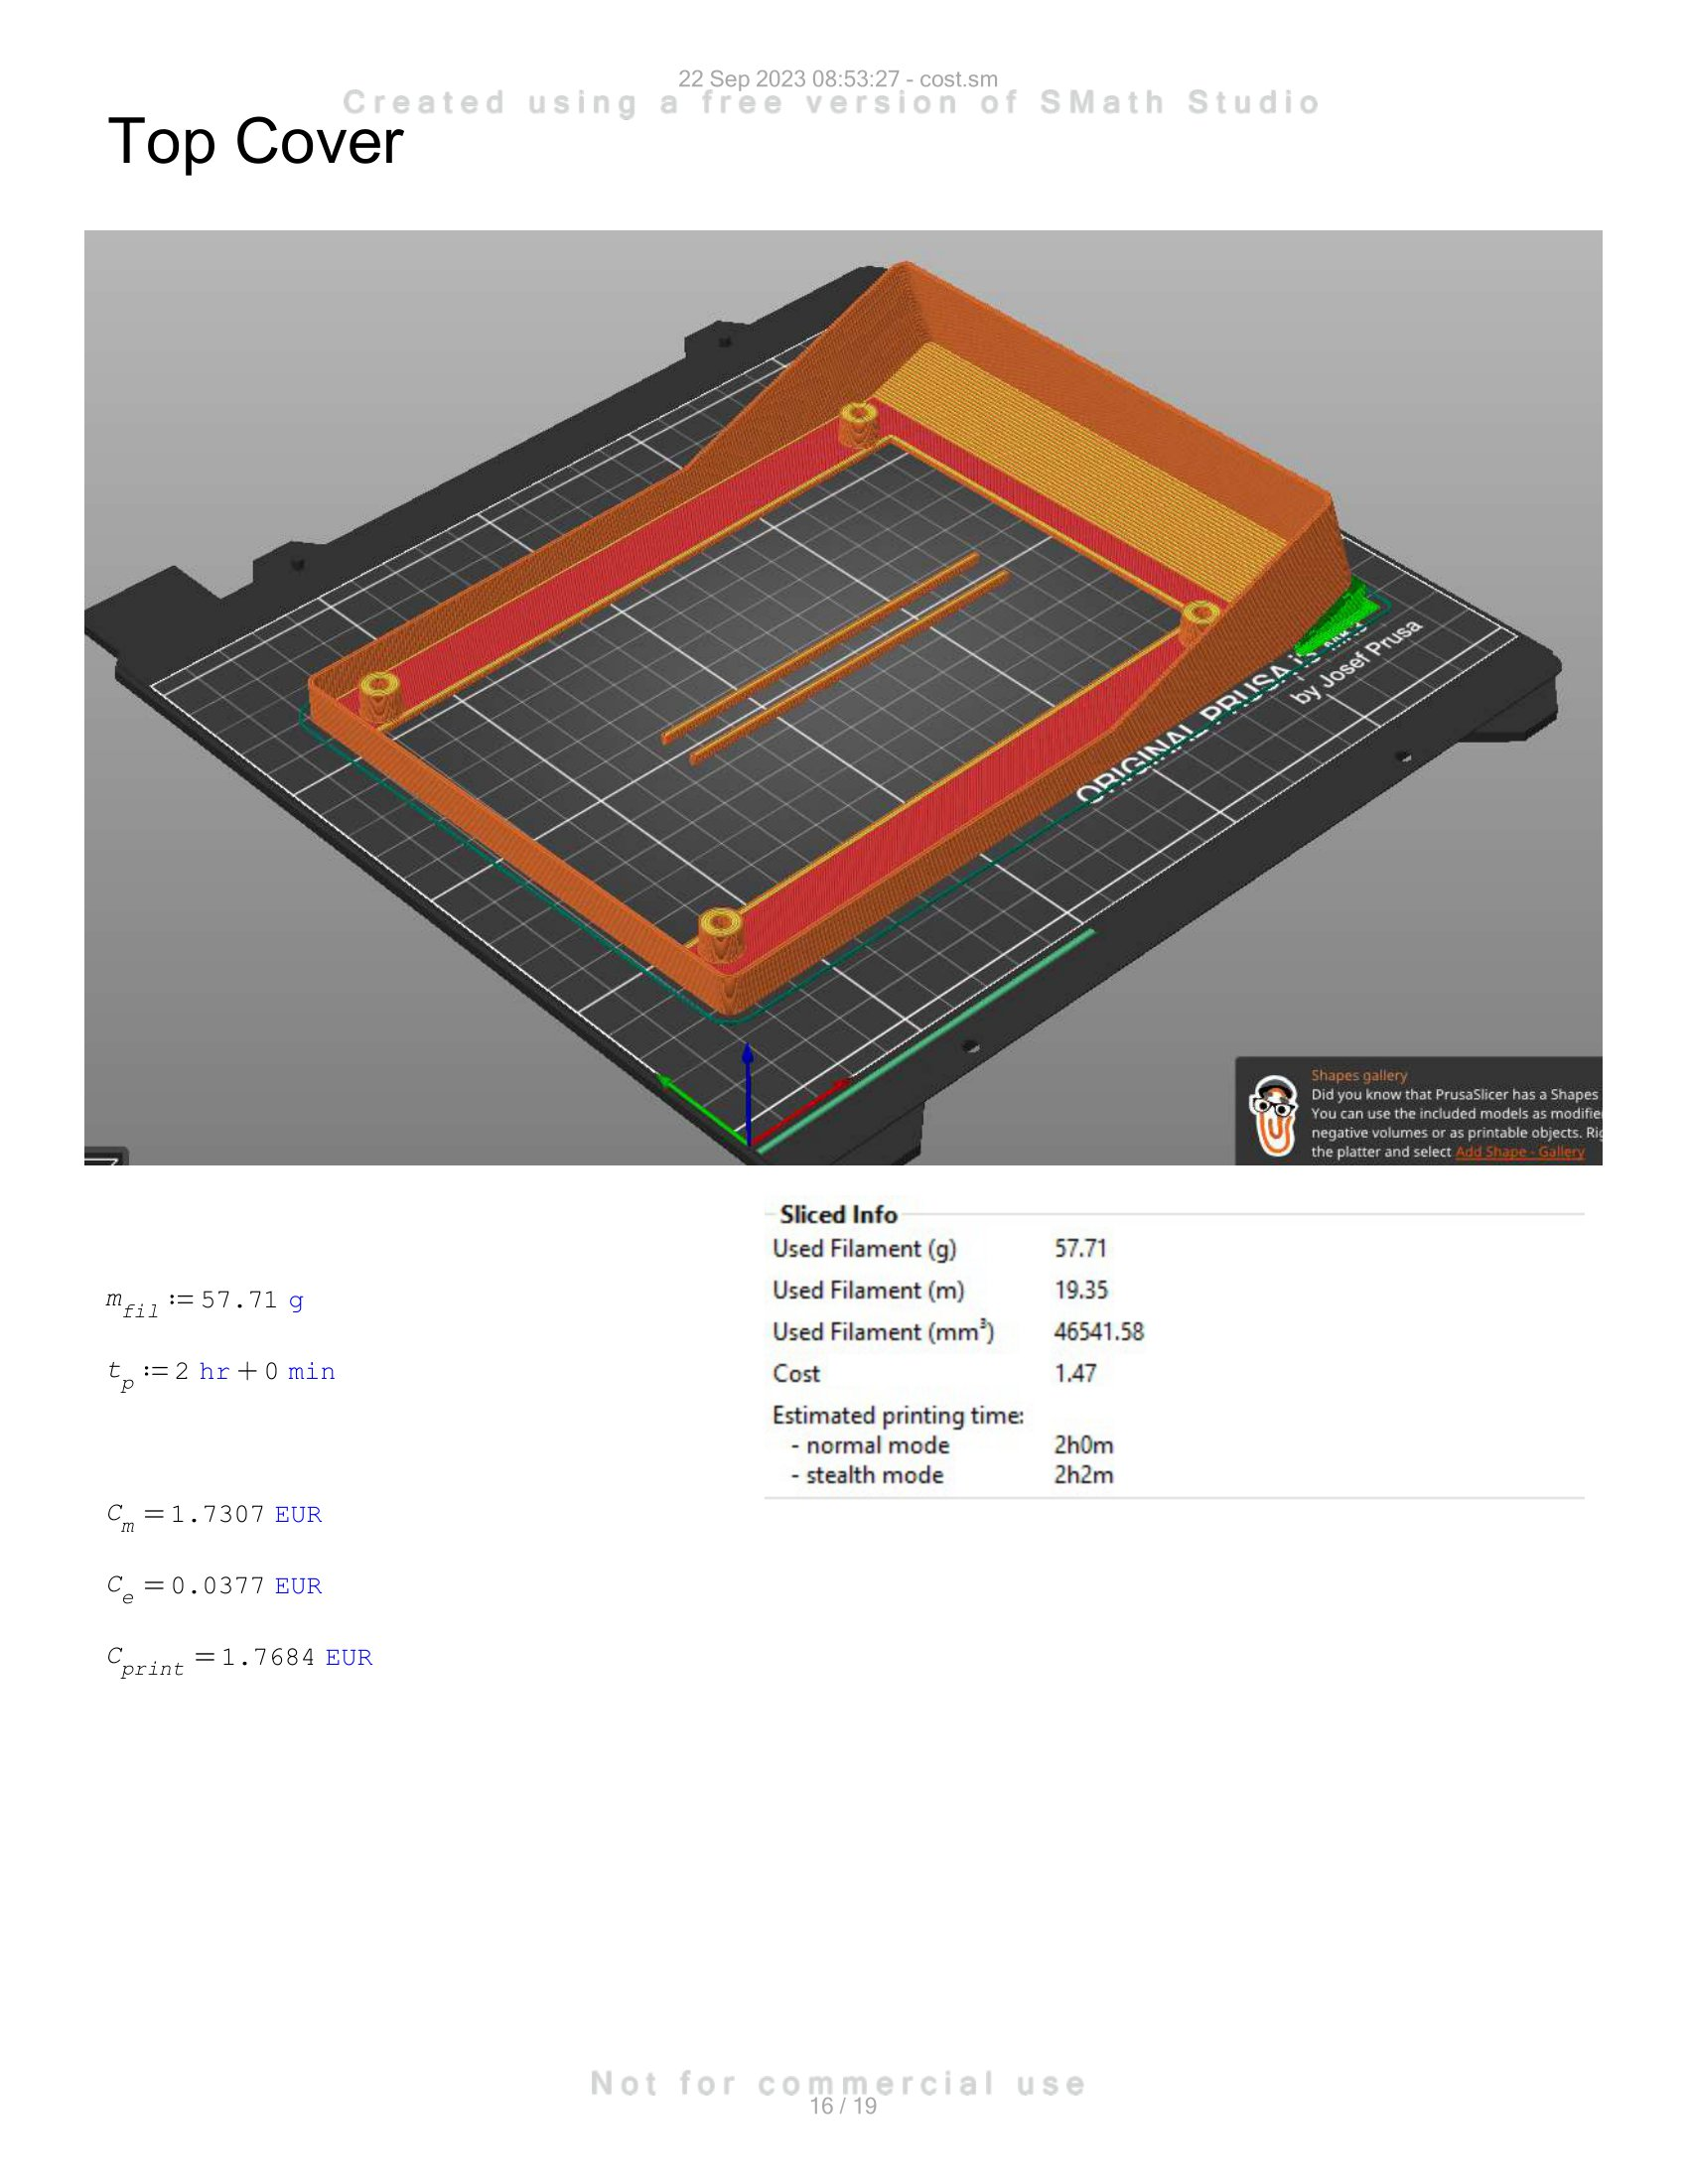
\includegraphics[width=\linewidth]{texs/appendix/data/costcalculation/cost1-16.jpg}
    \caption{Cost Calculation 16}
    \label{fig:cost-calculation-16}
\end{figure}

\begin{figure}[H]
    \centering
    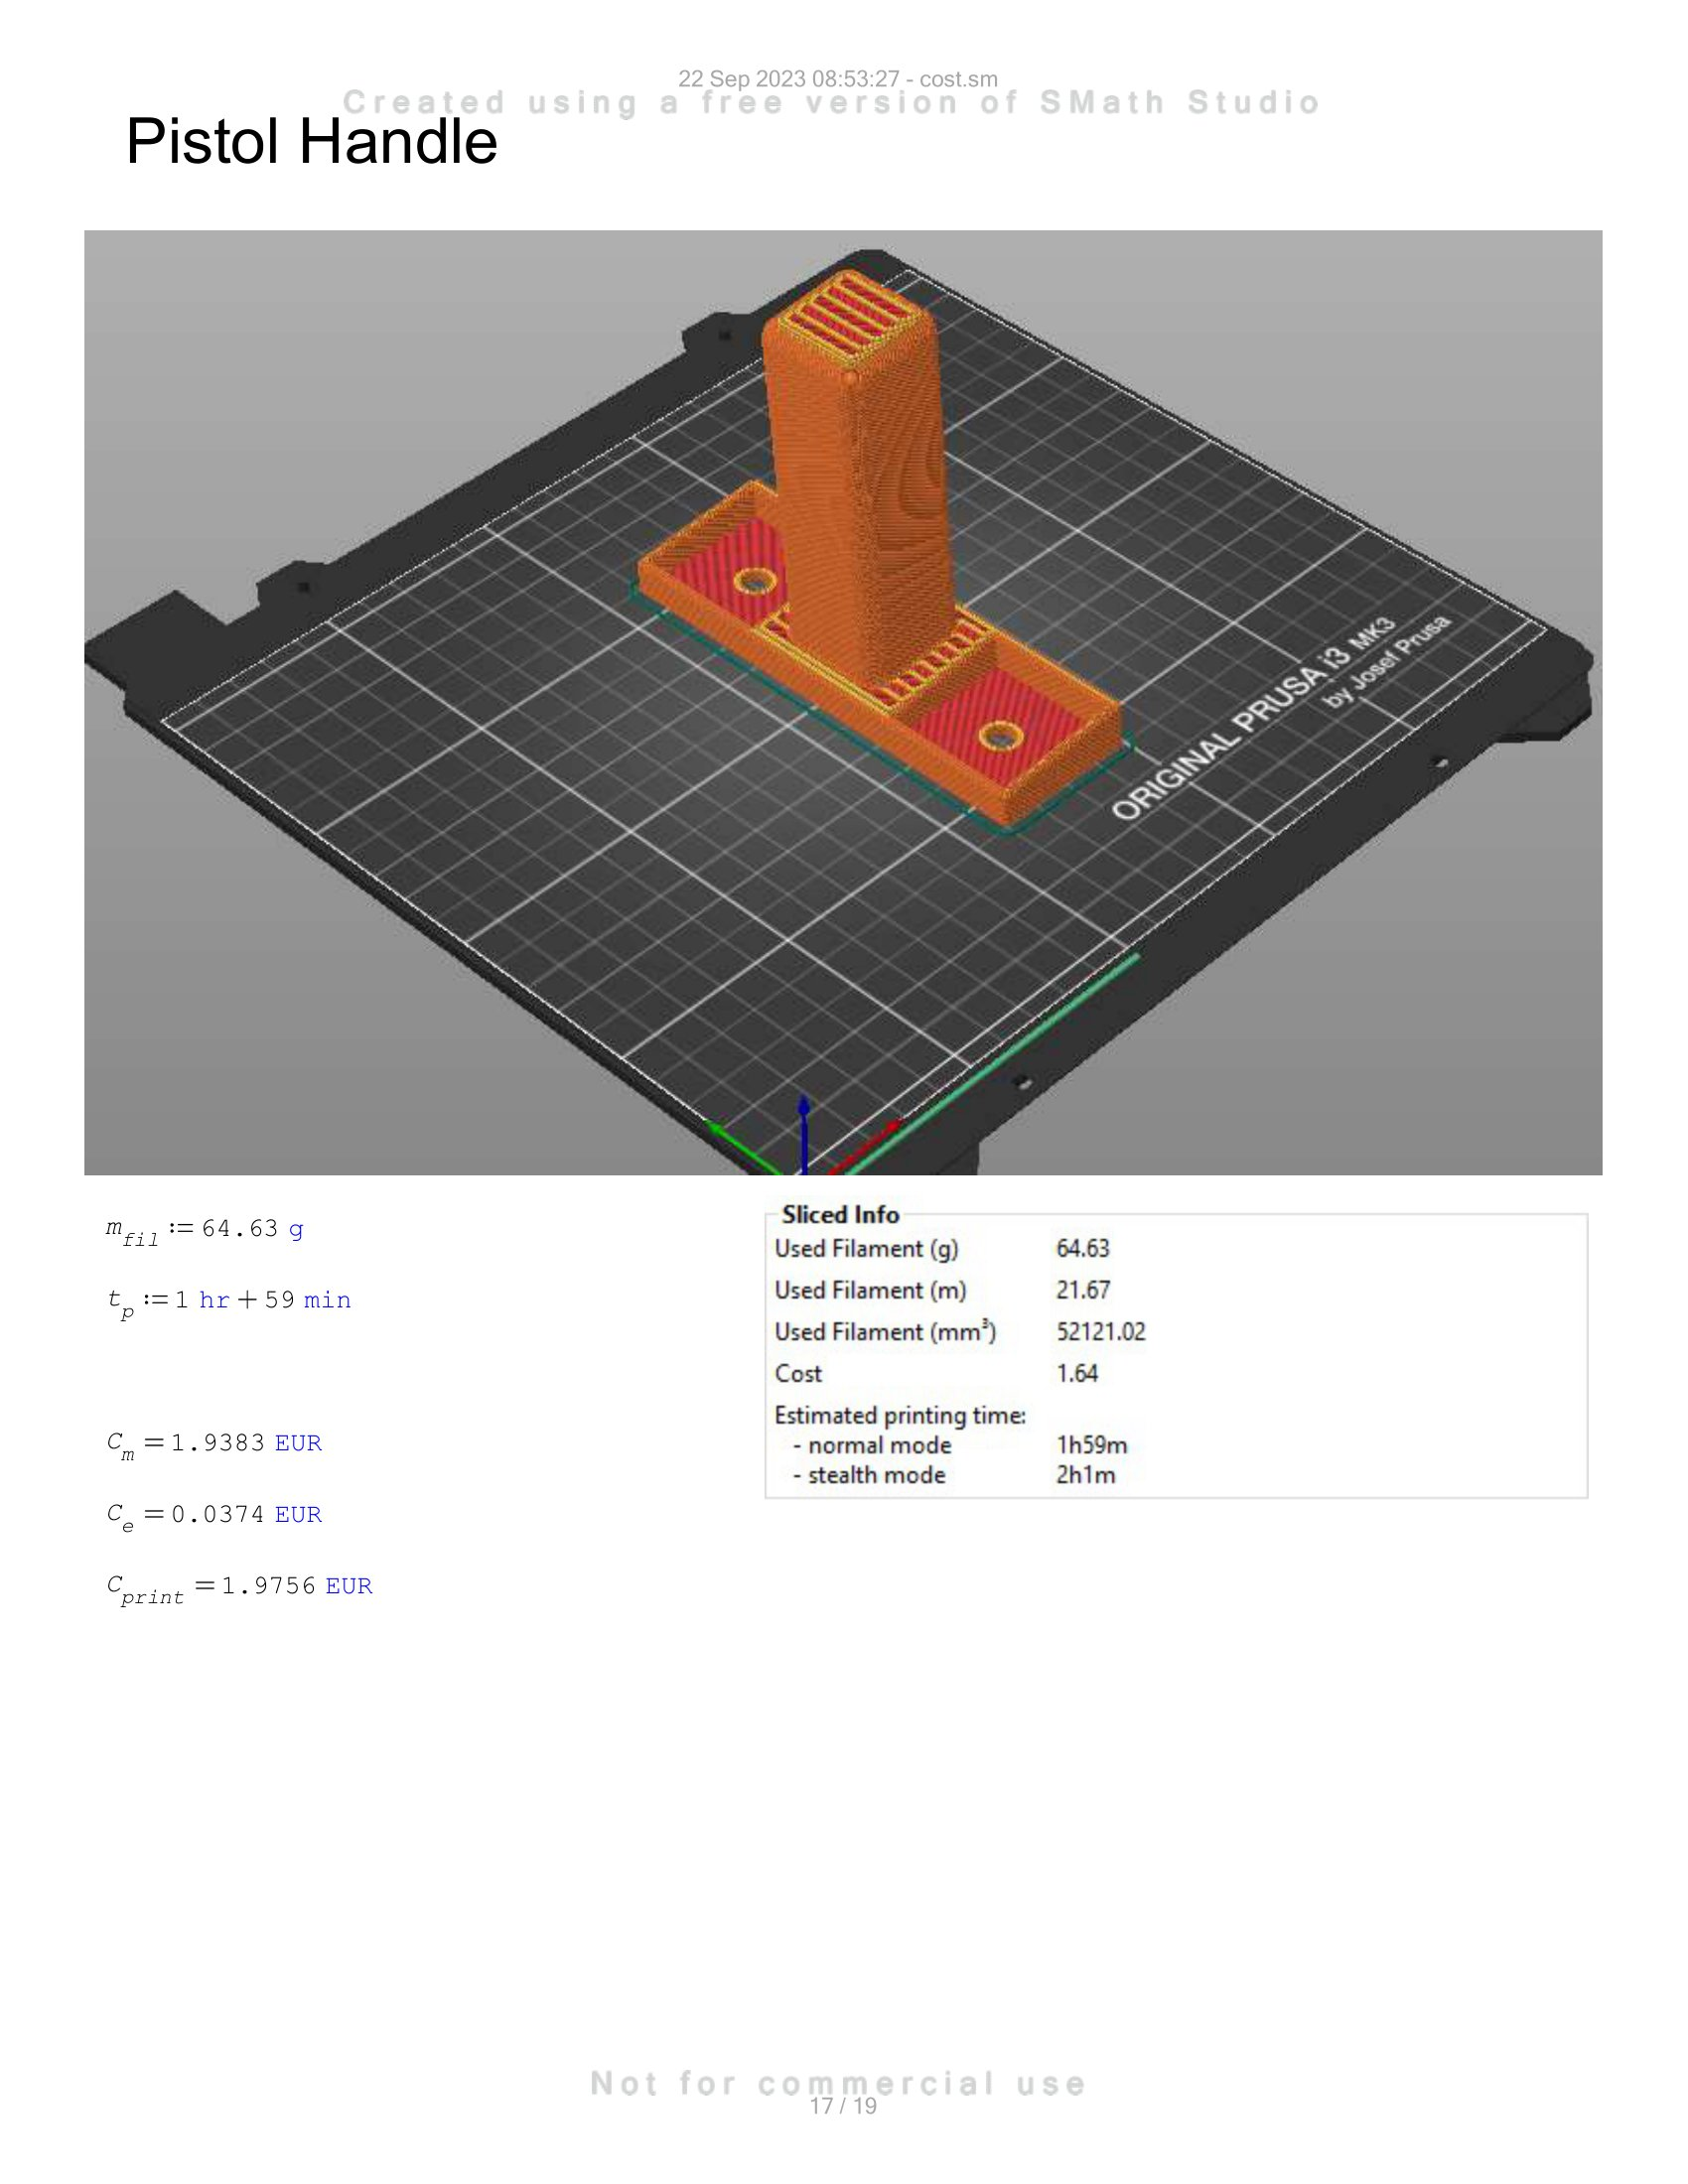
\includegraphics[width=\linewidth]{texs/appendix/data/costcalculation/cost1-17.jpg}
    \caption{Cost Calculation 17}
    \label{fig:cost-calculation-17}
\end{figure}

\begin{figure}[H]
    \centering
    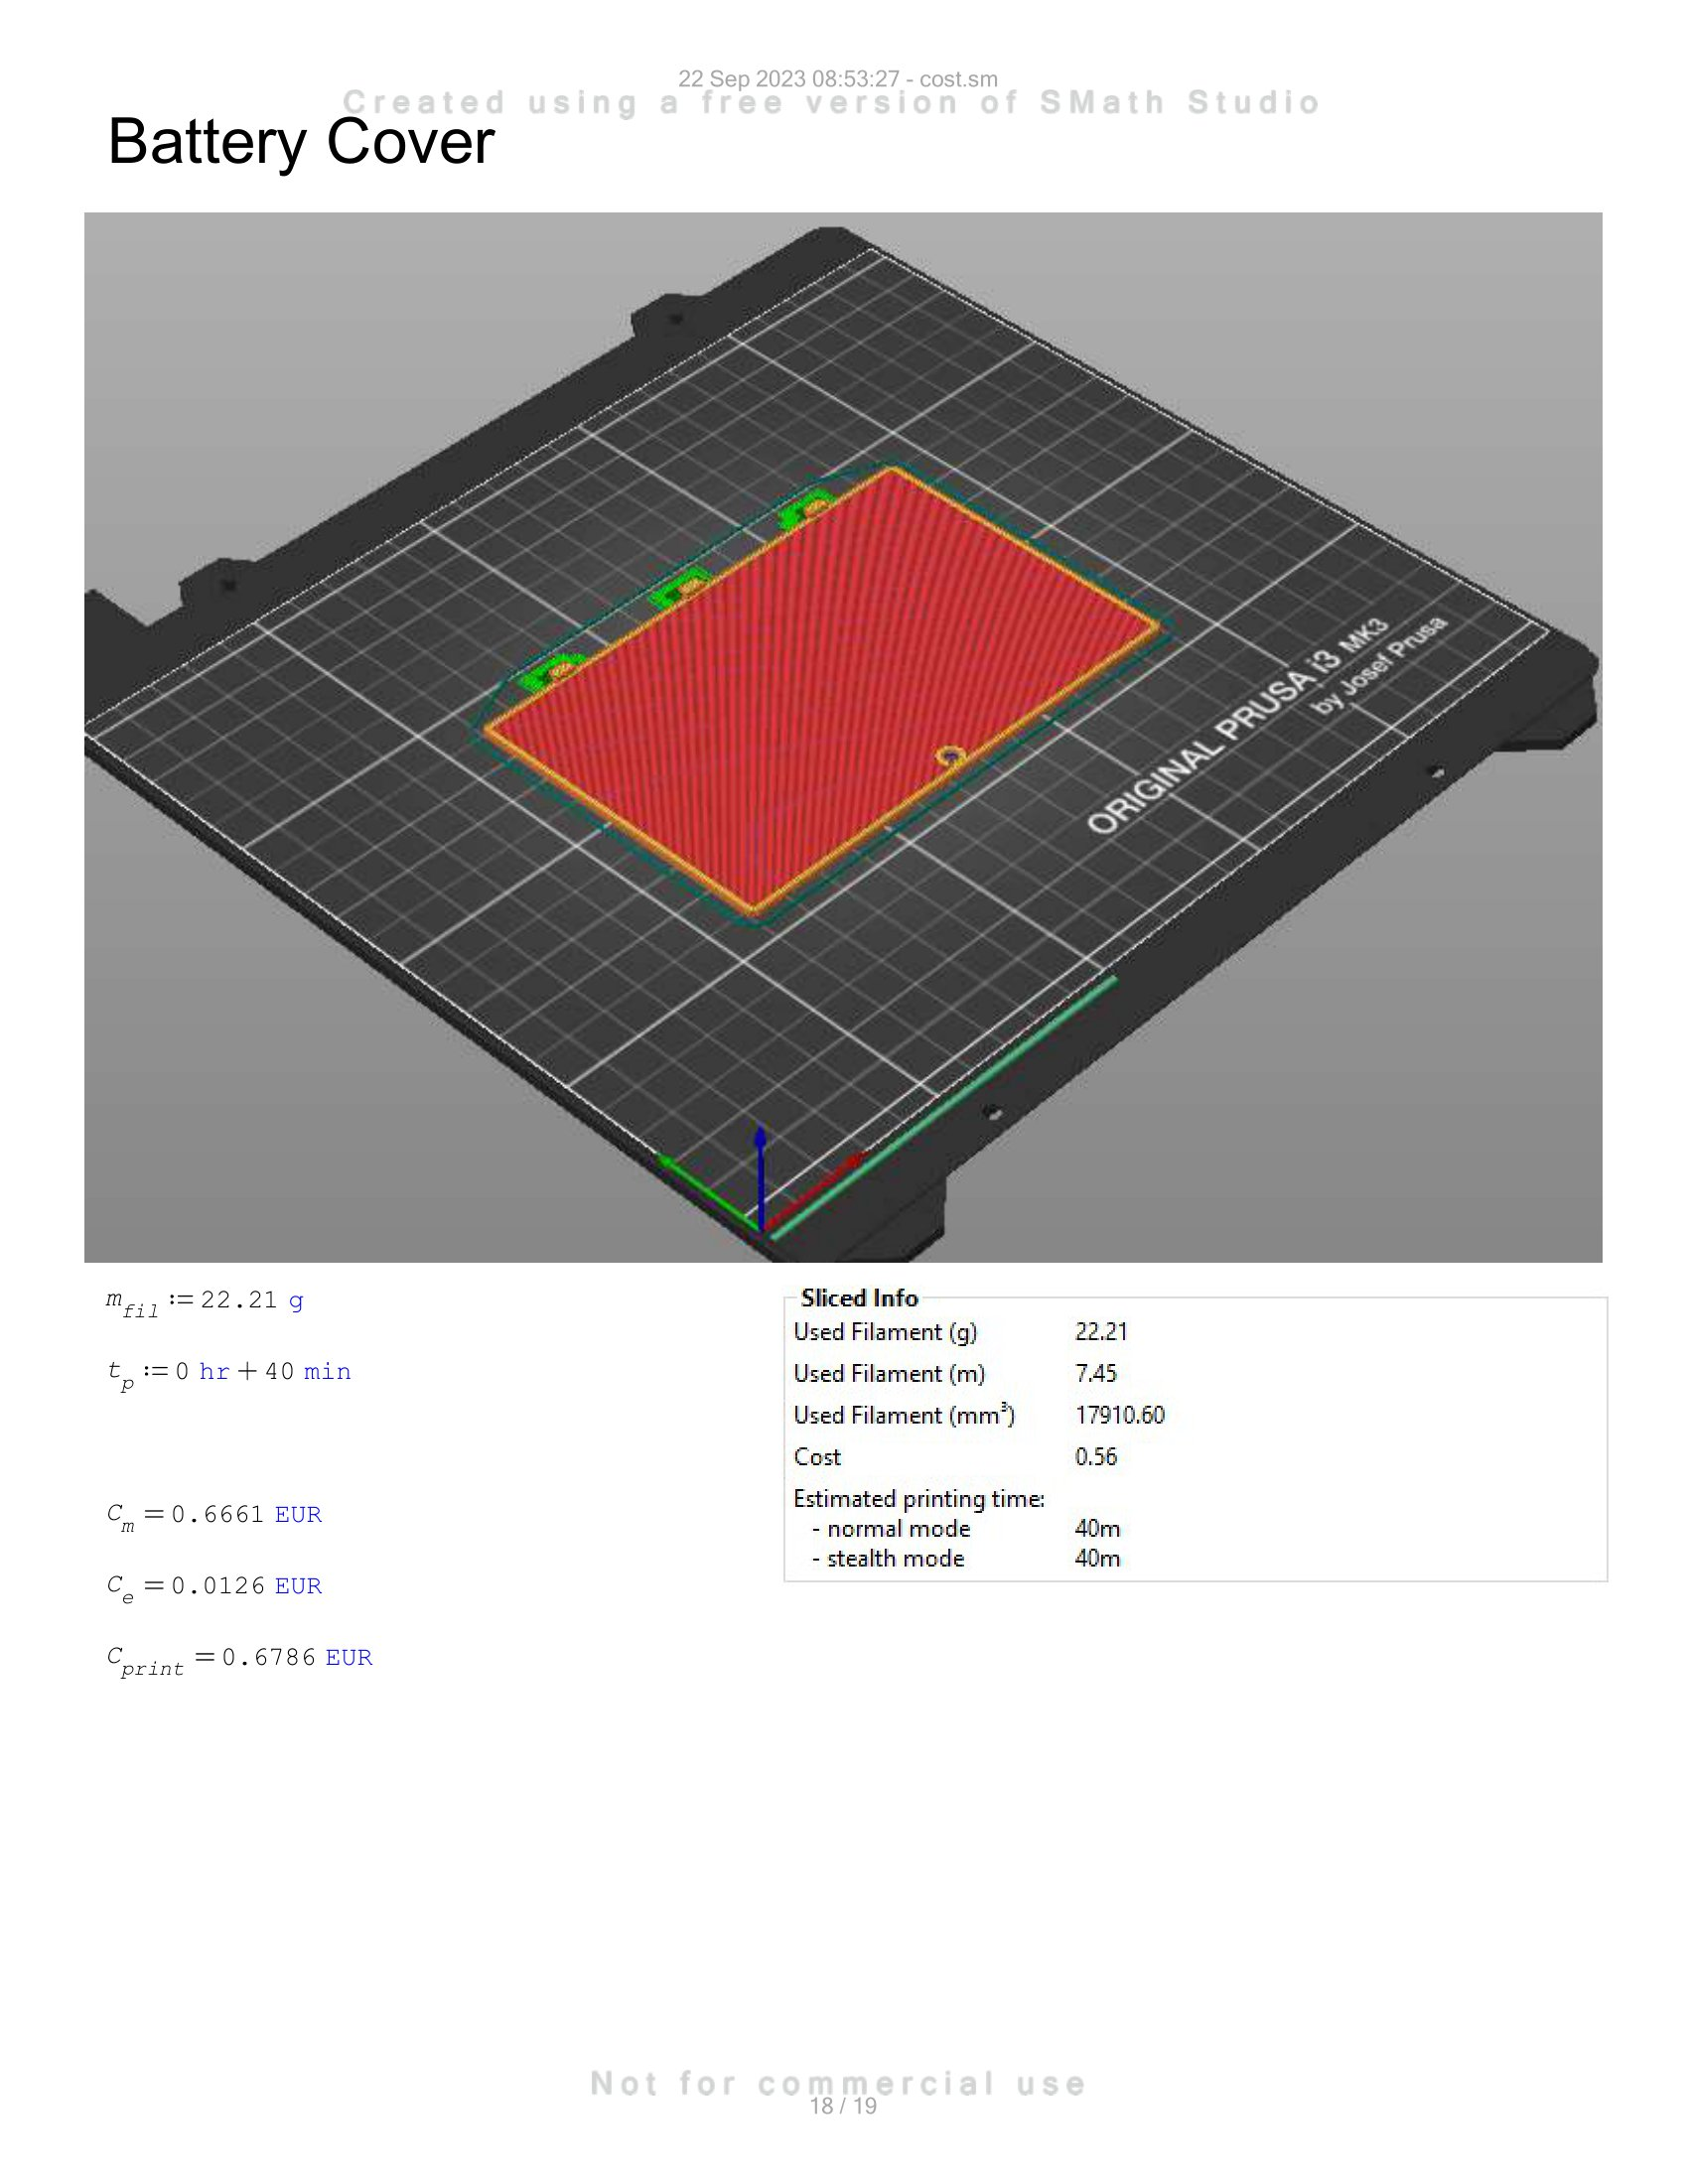
\includegraphics[width=\linewidth]{texs/appendix/data/costcalculation/cost1-18.jpg}
    \caption{Cost Calculation 18}
    \label{fig:cost-calculation-18}
\end{figure}

\begin{figure}[H]
    \centering
    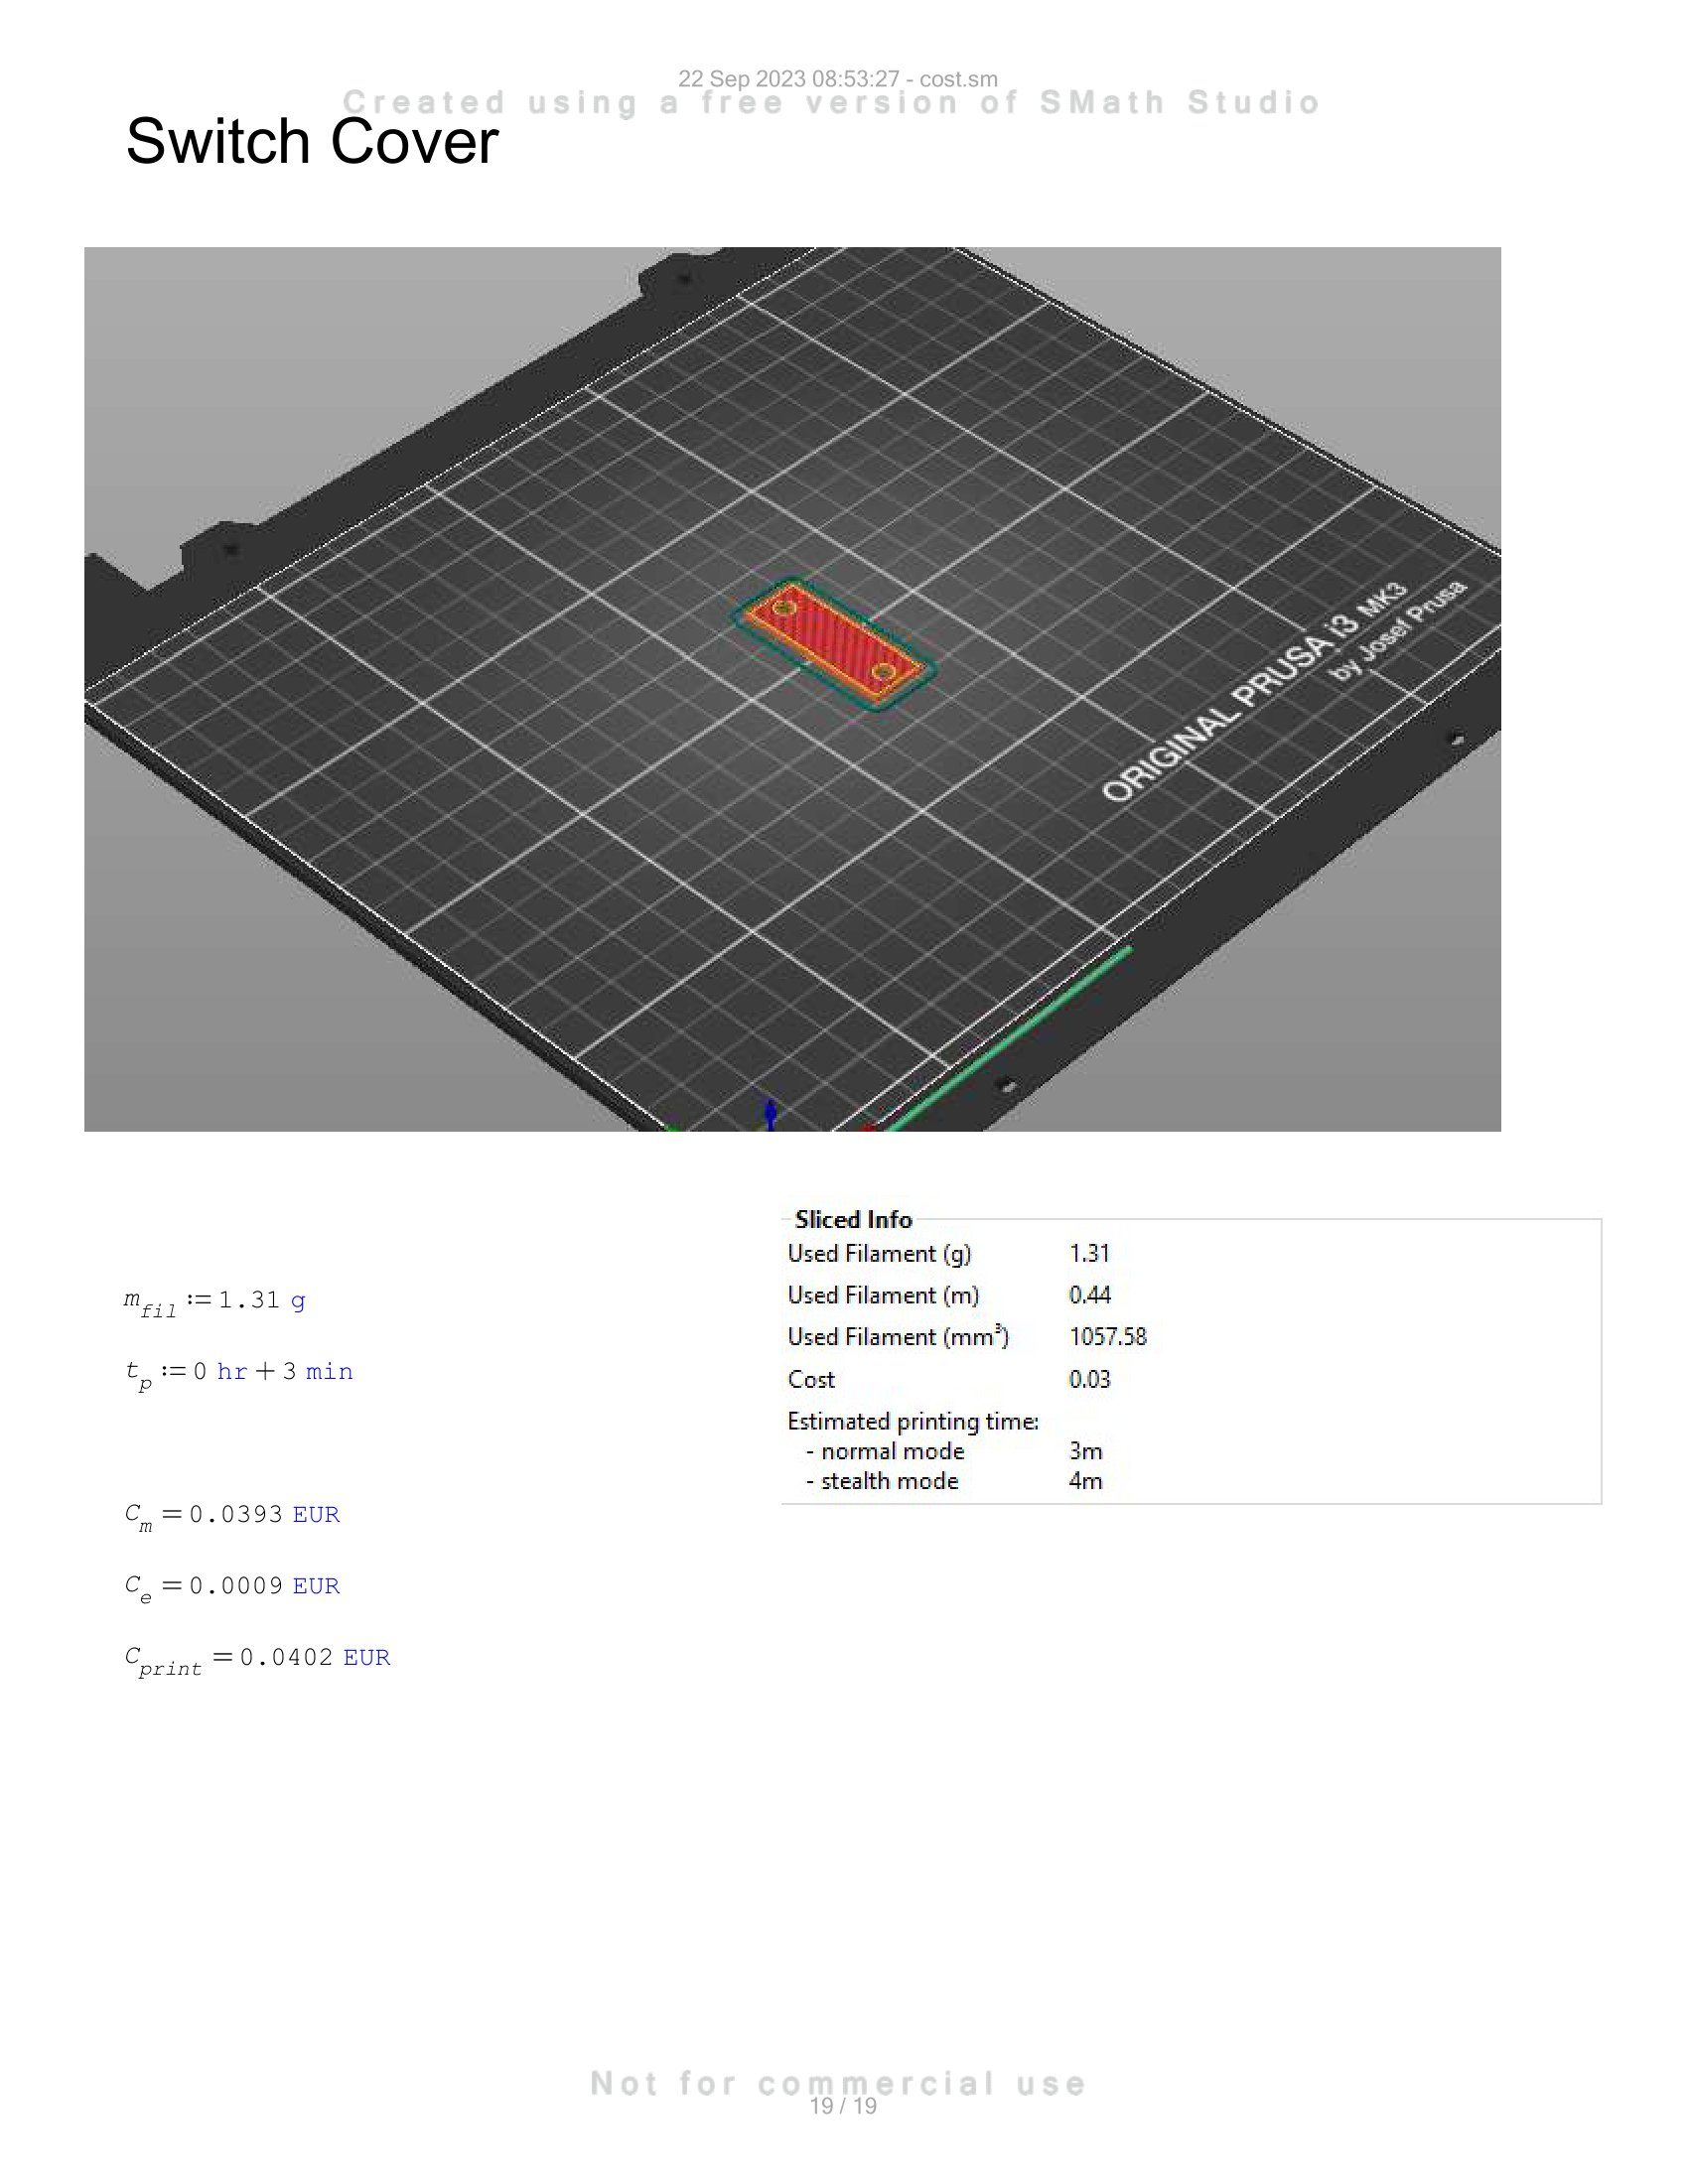
\includegraphics[width=\linewidth]{texs/appendix/data/costcalculation/cost1-19.jpg}
    \caption{Cost Calculation 19}
    \label{fig:cost-calculation-19}
\end{figure}

\section{Evaluation Data}
\label{appendix:evaluation-data}

\begin{figure}[H]
    \centering
    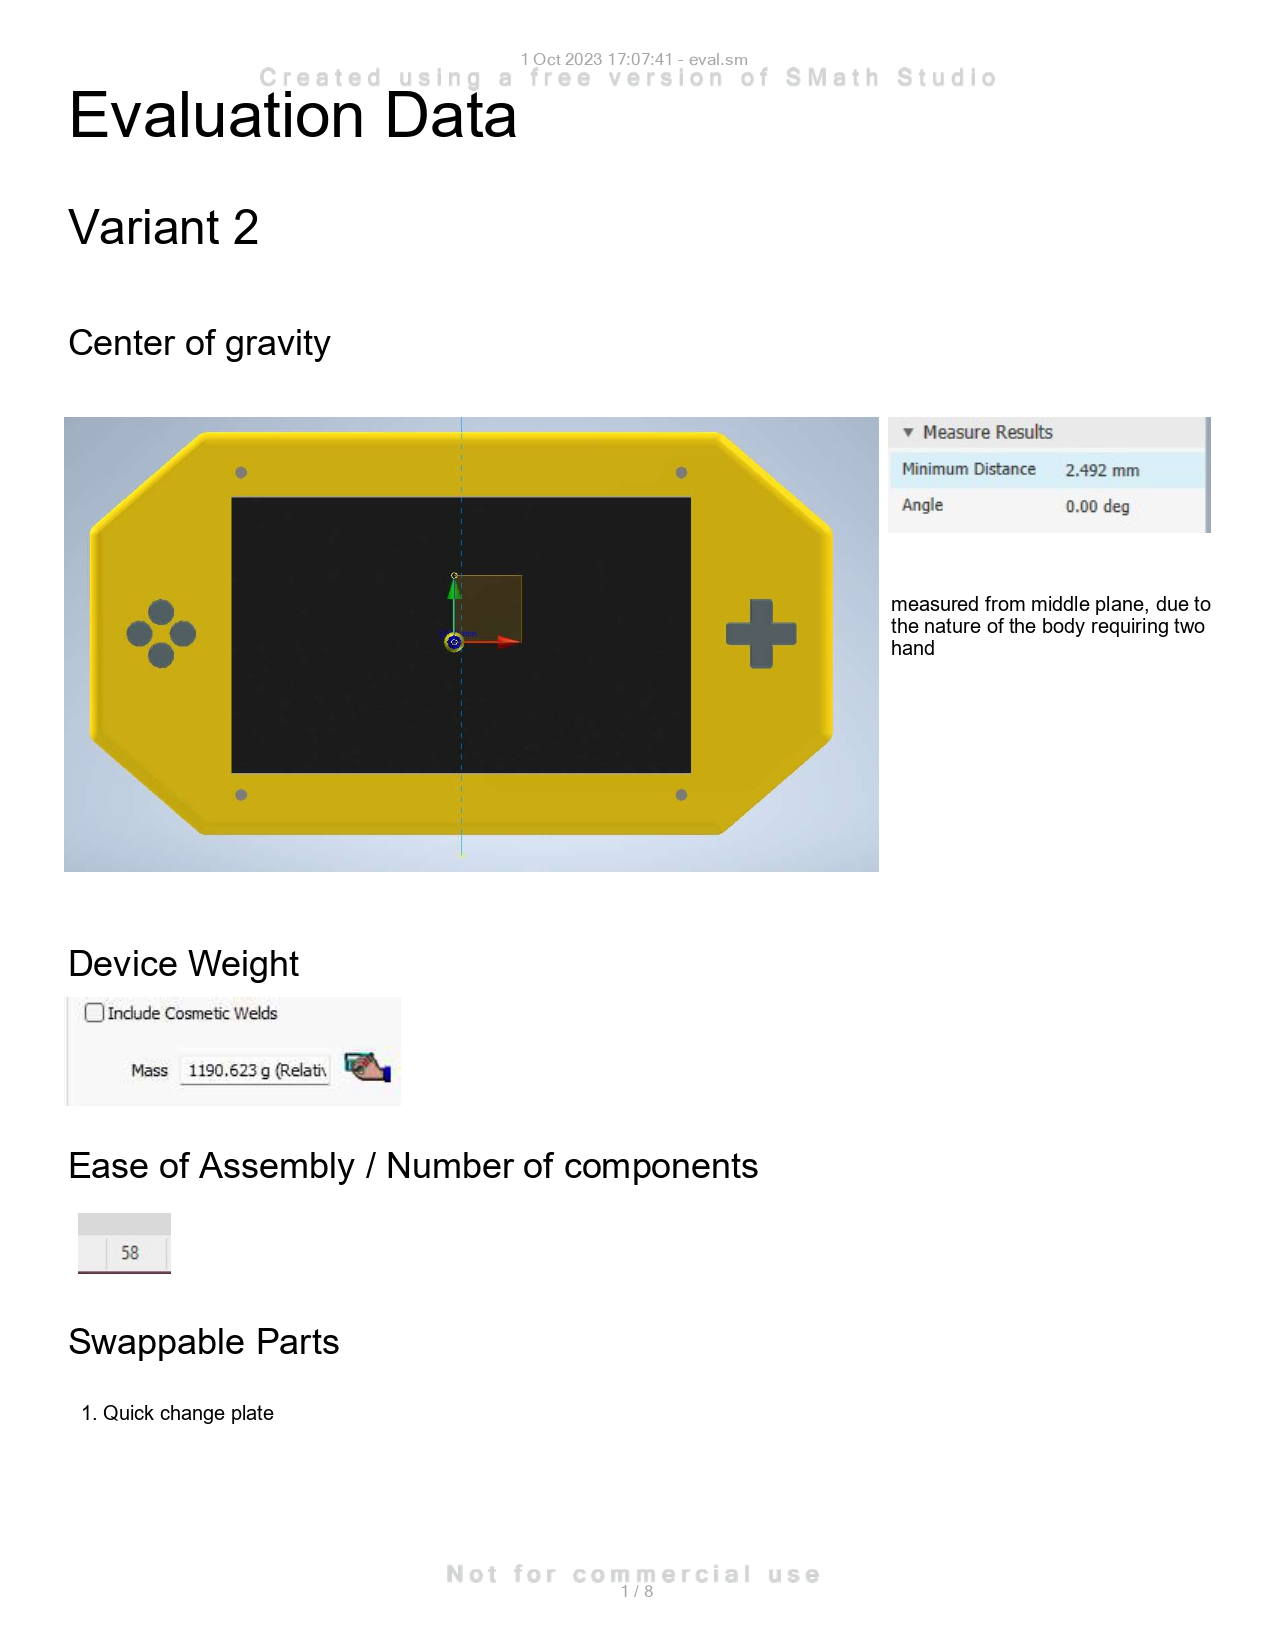
\includegraphics[width=\linewidth]{texs/appendix/data/evaluation/eval_page-0001.jpg}
    \caption{Evaluation 1}
    \label{fig:evaluation-1}
\end{figure}

\begin{figure}[H]
    \centering
    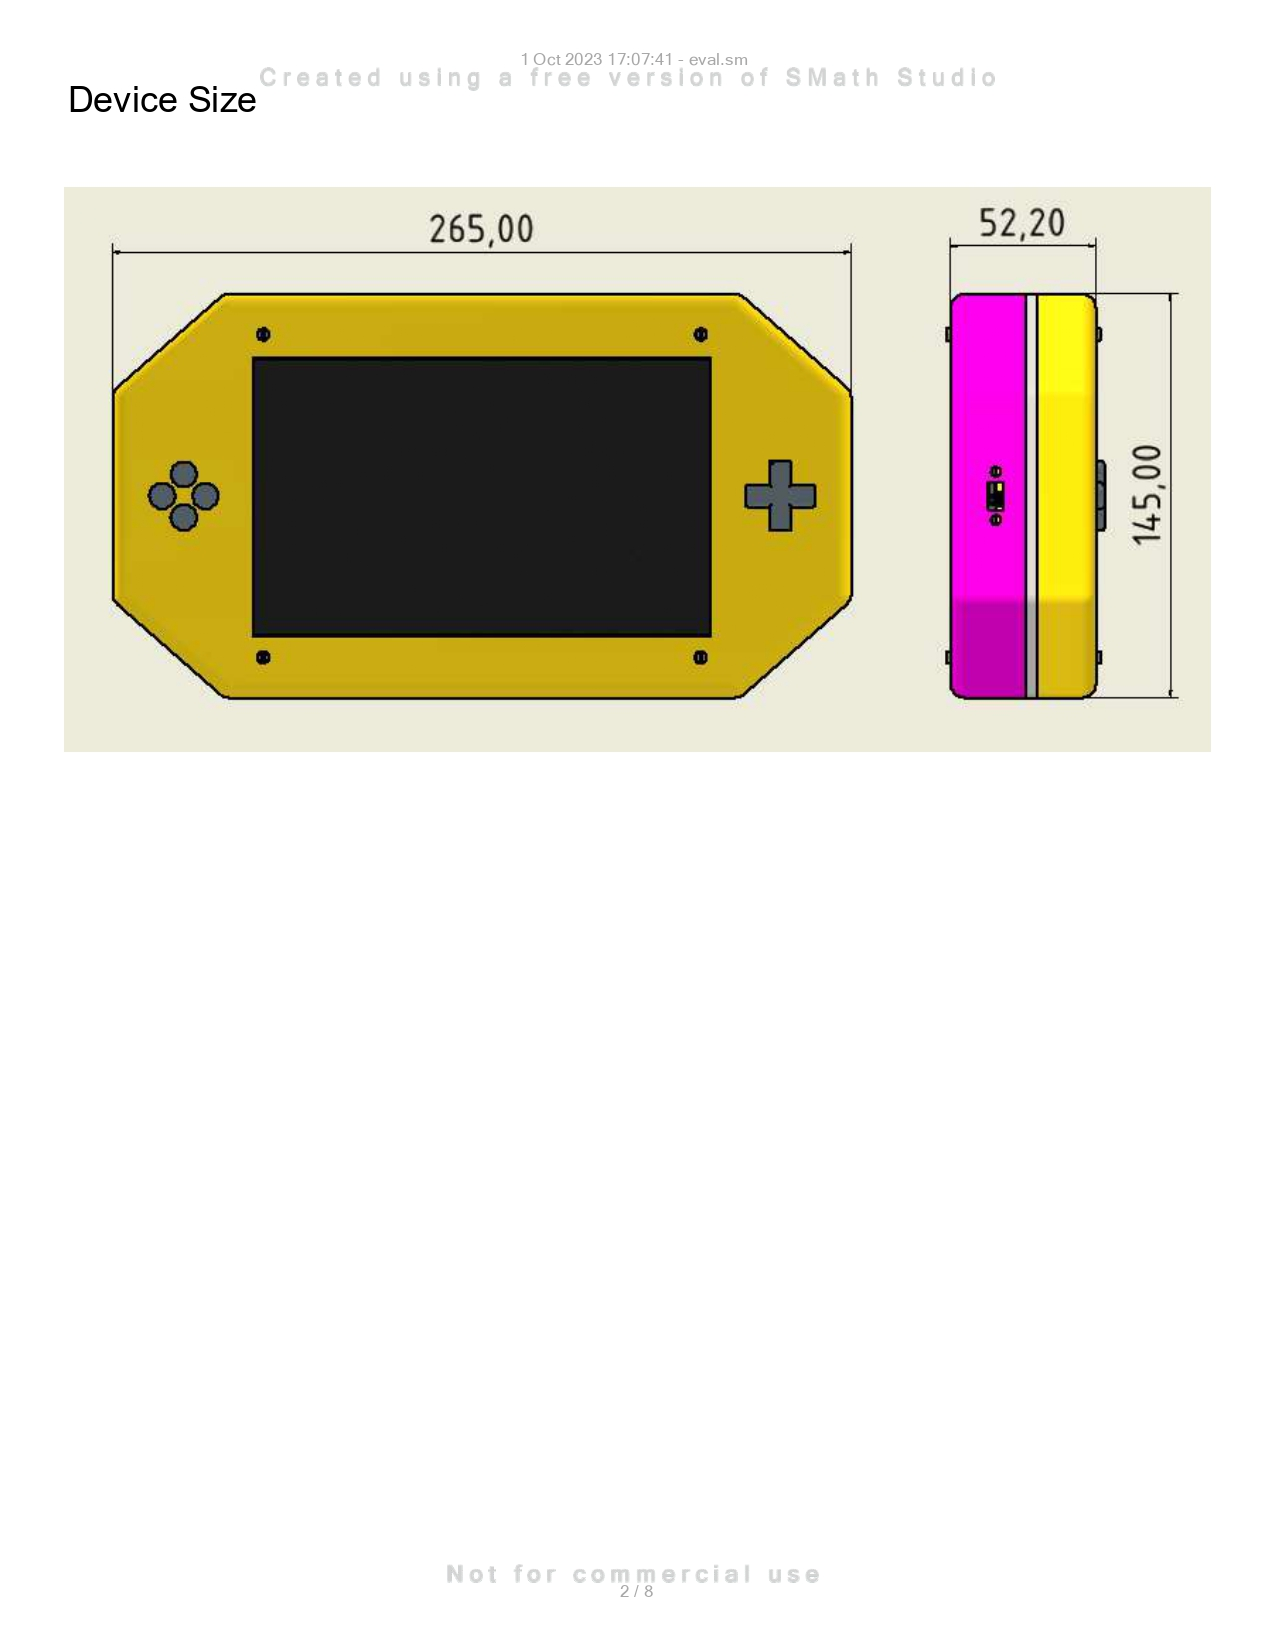
\includegraphics[width=\linewidth]{texs/appendix/data/evaluation/eval_page-0002.jpg}
    \caption{Evaluation 2}
    \label{fig:evaluation-2}
\end{figure}

\begin{figure}[H]
    \centering
    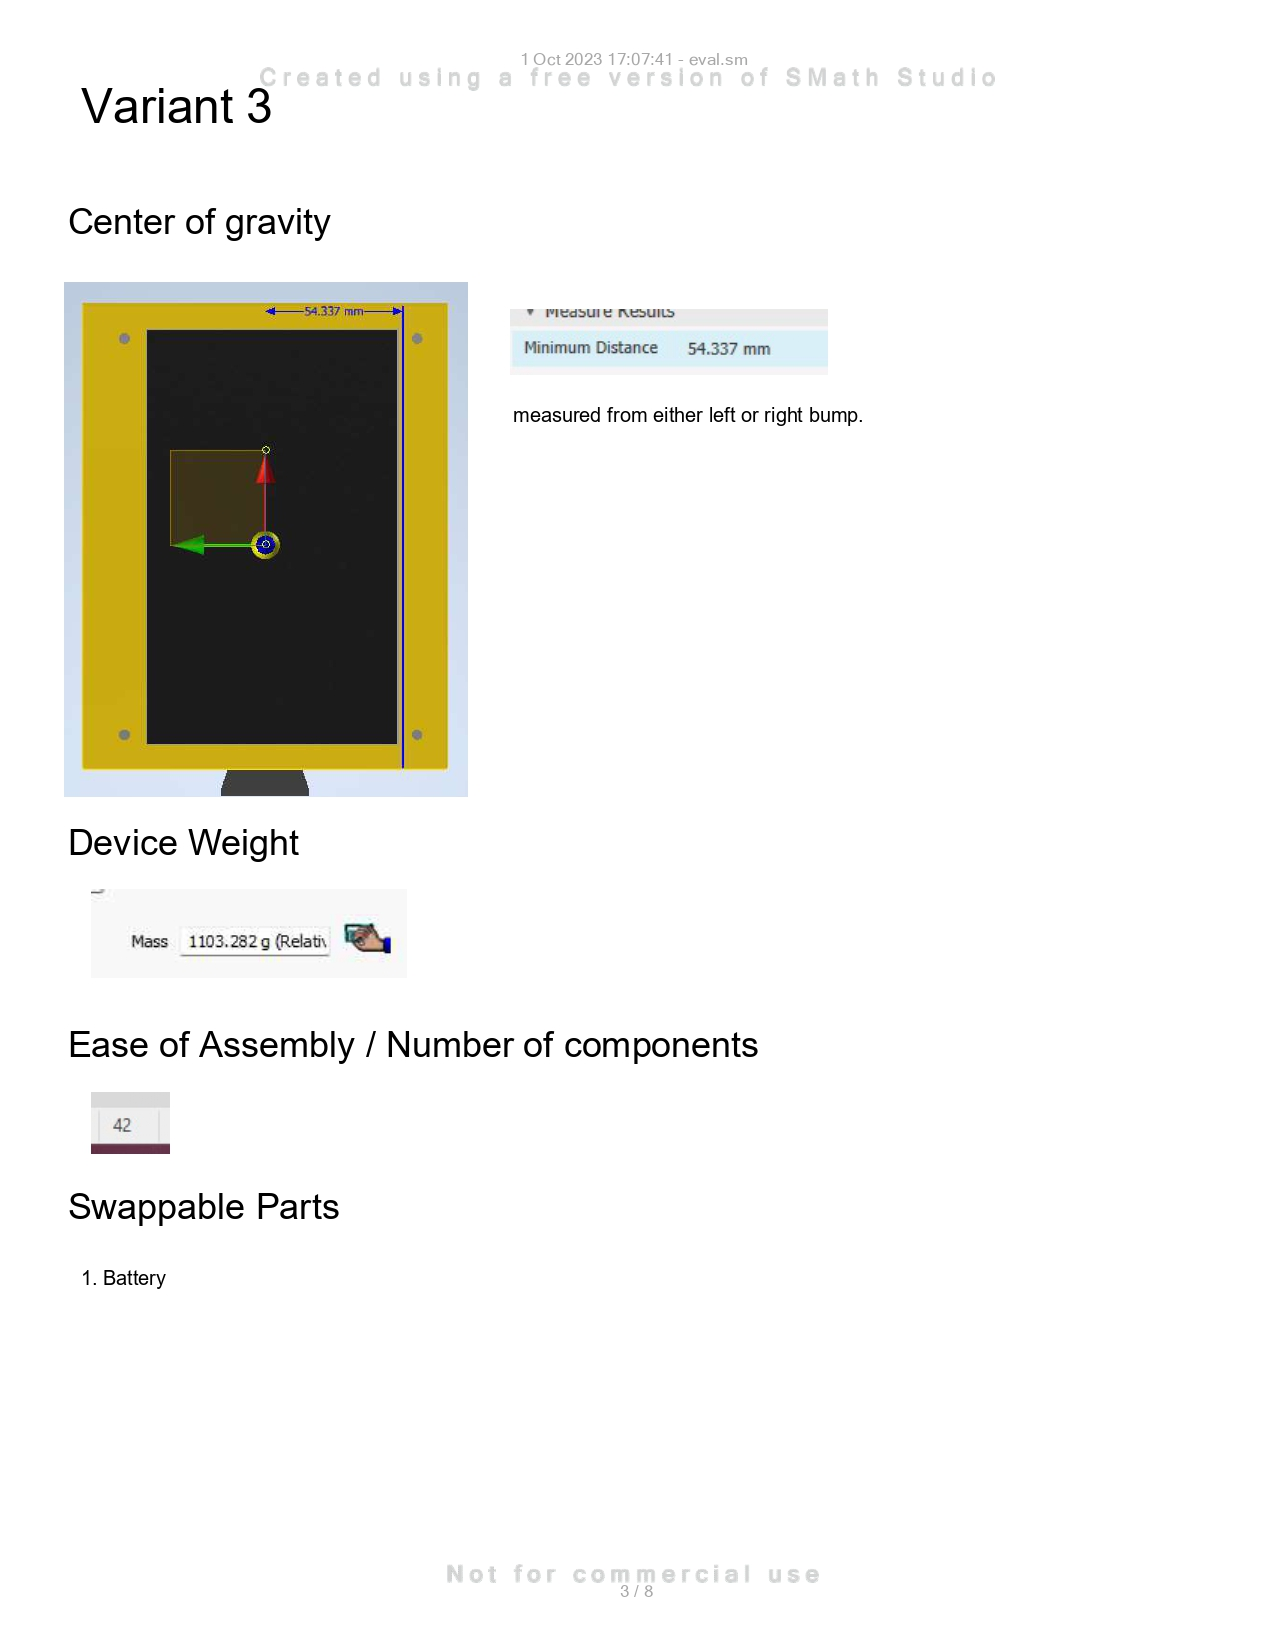
\includegraphics[width=\linewidth]{texs/appendix/data/evaluation/eval_page-0003.jpg}
    \caption{Evaluation 3}
    \label{fig:evaluation-3}
\end{figure}

\begin{figure}[H]
    \centering
    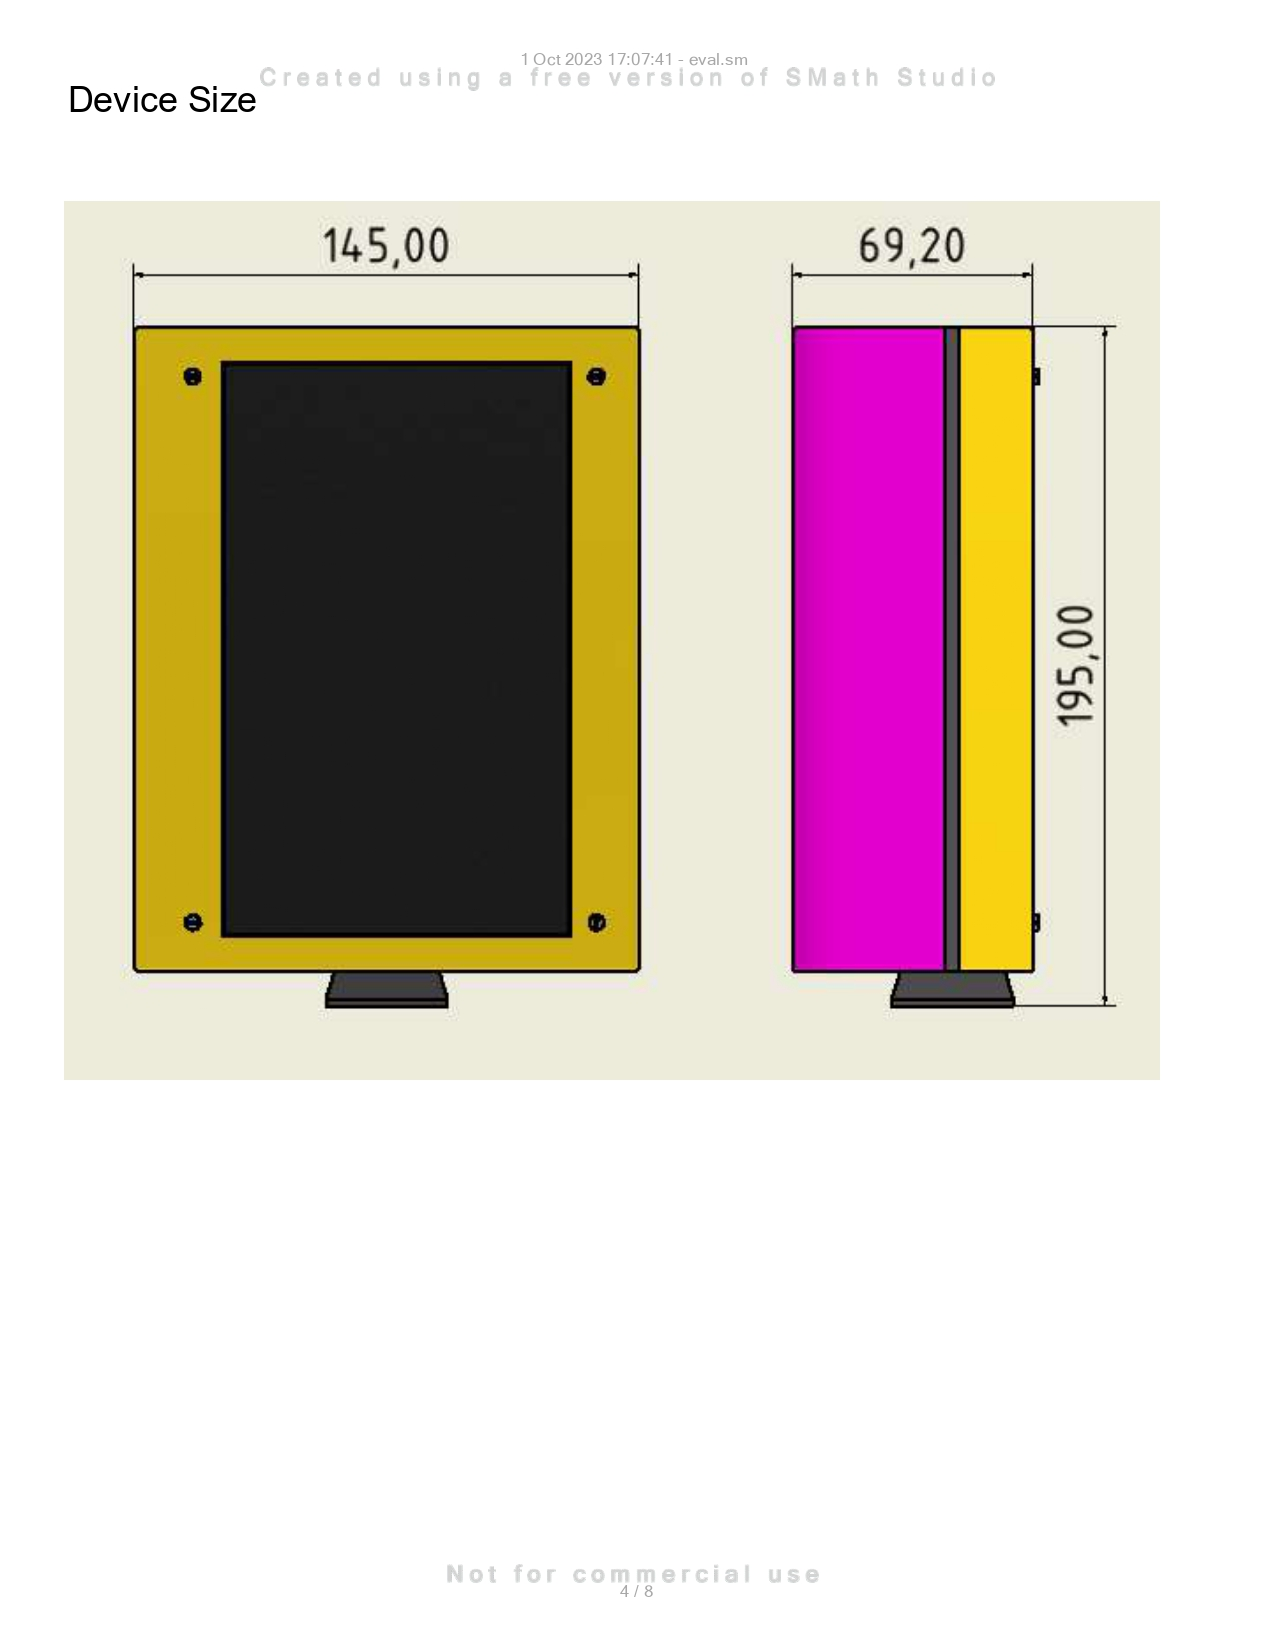
\includegraphics[width=\linewidth]{texs/appendix/data/evaluation/eval_page-0004.jpg}
    \caption{Evaluation 4}
    \label{fig:evaluation-4}
\end{figure}

\begin{figure}[H]
    \centering
    \includegraphics[width=\linewidth]{texs/appendix/data/evaluation/eval_page-0005.jpg}
    \caption{Evaluation 5}
    \label{fig:evaluation-5}
\end{figure}

\begin{figure}[H]
    \centering
    \includegraphics[width=\linewidth]{texs/appendix/data/evaluation/eval_page-0006.jpg}
    \caption{Evaluation 6}
    \label{fig:evaluation-6}
\end{figure}

\begin{figure}[H]
    \centering
    \includegraphics[width=\linewidth]{texs/appendix/data/evaluation/eval_page-0007.jpg}
    \caption{Evaluation 7}
    \label{fig:evaluation-7}
\end{figure}

\begin{figure}[H]
    \centering
    \includegraphics[width=\linewidth]{texs/appendix/data/evaluation/eval_page-0008.jpg}
    \caption{Evaluation 8}
    \label{fig:evaluation-8}
\end{figure}

\section{Documentation}

\begin{itemize}
    \item \href{https://haziqsabtu.github.io/SpeedCameraPi/}{Docs}
    \item \href{https://github.com/HaziqSabtu/SpeedCameraPi}{Repository}
\end{itemize}

\section{Code snippets}



%table of figures
%\clearpage
%\listoffigures
%\clearpage

%empty page 
% \thispagestyle{empty}
% \cleardoublepage

\end{document}
